% -- doc setup --
\documentclass[notitlepage,rmp,aps,10pt]{revtex4-1}
%\usepackage{soul}
%\newcommand{\hlc}[2][yellow]{ {\sethlcolor{#1} \hl{#2}} }
\usepackage{url}
\usepackage{graphicx}
\usepackage{xcolor}
\usepackage{hyperref}
\usepackage{amsmath}
\usepackage[caption=false]{subfig}
\usepackage{amstext}
\usepackage{multirow}
\usepackage{makecell}
\usepackage[utf8]{inputenc}
\usepackage{tabu}
%\usepackage{longtable}
\usepackage[figuresright]{rotating}
\usepackage{adjustbox}
\usepackage{placeins}

\newcommand{\MJ}{M{\footnotesize AJORANA}}
\newcommand{\Demo}{D{\footnotesize EMON\-STRAT\-OR}}
\newcommand{\MJD}{\MJ\ \Demo}
\newcommand{\Gerda}{\textsc{Gerda}}
\newcommand{\bb}{${\beta \beta}$}
\newcommand{\znbb}{${0 \nu \beta \beta}$}
\newcommand{\tnbb}{${2 \nu \beta \beta}$}
\newcommand{\bbes}{\bb~E.S.}
\newcommand{\hl}[1]{$T^{#1}_{1/2}$}
\newcommand{\mbb}{$m_{\beta\beta}$}
\newcommand{\Qbb}{$Q_{\beta\beta}$}
\newcommand{\Qval}{$Q$-value}
\newcommand{\Mage}{\textsc{MaGe}}
\newcommand{\geant}{\textsc{Geant4}}
\newcommand{\cpp}{C\protect\raisebox{.25ex}{++}\ }  % formats C++ correctly
\newcommand{\TTree}{\texttt{TTree}}

%isotope macros
\newcommand{\iso}[2]{$^{#1}$#2}
\newcommand{\Ge}[1]{\iso{#1}{Ge}}
\newcommand{\Se}[1]{\iso{#1}{Se}}
\newcommand{\Th}[1]{\iso{#1}{Th}}
\newcommand{\Co}[1]{\iso{#1}{Co}}
\newcommand{\Tl}[1]{\iso{#1}{Tl}}
\newcommand{\Bi}[1]{\iso{#1}{Bi}}

%spin parity state macros
\newcommand{\SP}[3]{$#1^{#2}_{#3}$}
\newcommand{\gs}{\SP{0}{+}{g.s.}}
\newcommand{\decaySP}[3]{$0^+_{g.s.}\xrightarrow{#1\nu\beta\beta}#2^+_{#3}$}

\newcommand{\sd}{single-detector event}
\newcommand{\md}{multi-detector event}
\newcommand{\msmd}{multi-site event}
\newcommand{\mssd}{multi-site waveform}
\newcommand{\Md}{Multi-detector event}
\newcommand{\Msmd}{Multi-site event}
\newcommand{\Mssd}{Multi-site waveform}



\setcitestyle{numbers,square}

% -- make the very pretty and totally essential unidoc header --
\usepackage{fancyhdr}
\newcommand{\docno}{2019-042}
\definecolor{blue}{RGB}{50,0,255}
\definecolor{orange}{RGB}{255,128,0}
\colorlet{blueh}{blue!30}
\fancypagestyle{uniheader}
{
\fancyhf{}
\fancyhead[L]{Unidoc \#-\docno}
  \fancyfoot[C]{-\thepage-}
  \renewcommand{\headrulewidth}{2pt}
  \renewcommand{\headheight}{52pt}
  \renewcommand{\headrule}{\hbox to\headwidth{
    \color{orange}\leaders\hrule height \headrulewidth\hfill}}
  \renewcommand{\footrulewidth}{0pt}
  \rhead{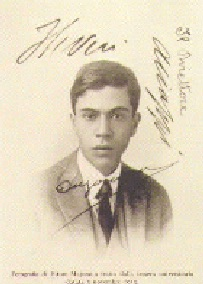
\includegraphics[width=1cm]{Ettore}}
}

% -- custom environs --
\newenvironment{itemize_nospace}
{ \begin{itemize}
    \setlength{\itemsep}{3pt}
    \setlength{\parskip}{0pt}
    \setlength{\parsep}{0pt}     }
{ \end{itemize}                  }
\newcommand{\tty}{\texttt}

\usepackage{lineno}
\linenumbers

%%%%%%%%%%%%%%%%%%%%% BEGIN DOCUMENT %%%%%%%%%%%%%%%%%%%%%%

\begin{document}
\graphicspath{{./pics/}{../ch3/pics/}{../ch4/pics/}{../ch5/pics/}{../appAllResults/pics/}{../appSens/pics/}}

\title{Search for Double Beta Decay to Excited States}
\author{I. Guinn}\affiliation{University of North Carolina at Chapel Hill, NC, USA}

\pagestyle{uniheader}
\maketitle
\vspace*{-1.5cm}
\tableofcontents
\thispagestyle{uniheader}

\section{Introduction}
\Se{76} has 3 excited states that \Ge{76} can decay into in addition to the ground state, as shown in figure~\ref{fig:Ge76BBLevelDiagram}.
While the ground state decay has been observed, none of the decays to excited states have been yet.
Each excited state decay will have a \bb -decay with a reduced \Qval\ compared to the ground state decay.
The excited state decays will also promptly produce one or two $\gamma$-rays at known energies.
These $\gamma$s will typically travel several centimeters before absorption and will often hit a different detector from the \bb -decay site, meaning that we can search for peaks at these energies.
\\
\begin{figure}[h]
  \centering
  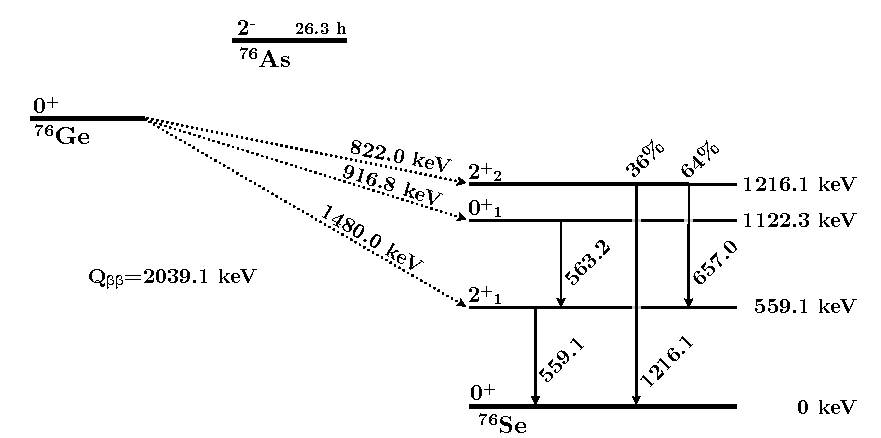
\includegraphics[width=0.8\textwidth]{leveldiagram}
  \caption[Energy level diagram for \Ge{76} \bb to \Se{76}]{\label{fig:Ge76BBLevelDiagram}
    Energy level diagram for \bb-decay of \Ge{76} to \Se{76}, including excited states. The \Qval s for each decay branch and the energies and branching ratios for the deexcitation $\gamma$s are shown next to their corresponding lines.
  }
\end{figure}


Furthermore, since these $\gamma$s hit separate detectors, this signal is inherently \msmd.
As shown in figure~\ref{fig:multhist}, by searching for the peak only in events with high hit multiplicity, i.e. events that involve 2 or more detectors hit, $\sim85\%$ of backgrounds can be cut, while only sacrificing $\sim25$\% of the signal.
Furthermore, the coincident detector hit(s) can provide additional observables that can be used to further discriminate excited state signals from multi-site backgrounds.
This chapter will describe the various background reduction data cuts and how they are implemented.
It will also evaluate the detection efficiency and systematic error associated with each cut based on simulations of the \MJD.

\begin{figure}[h]
  \centering
  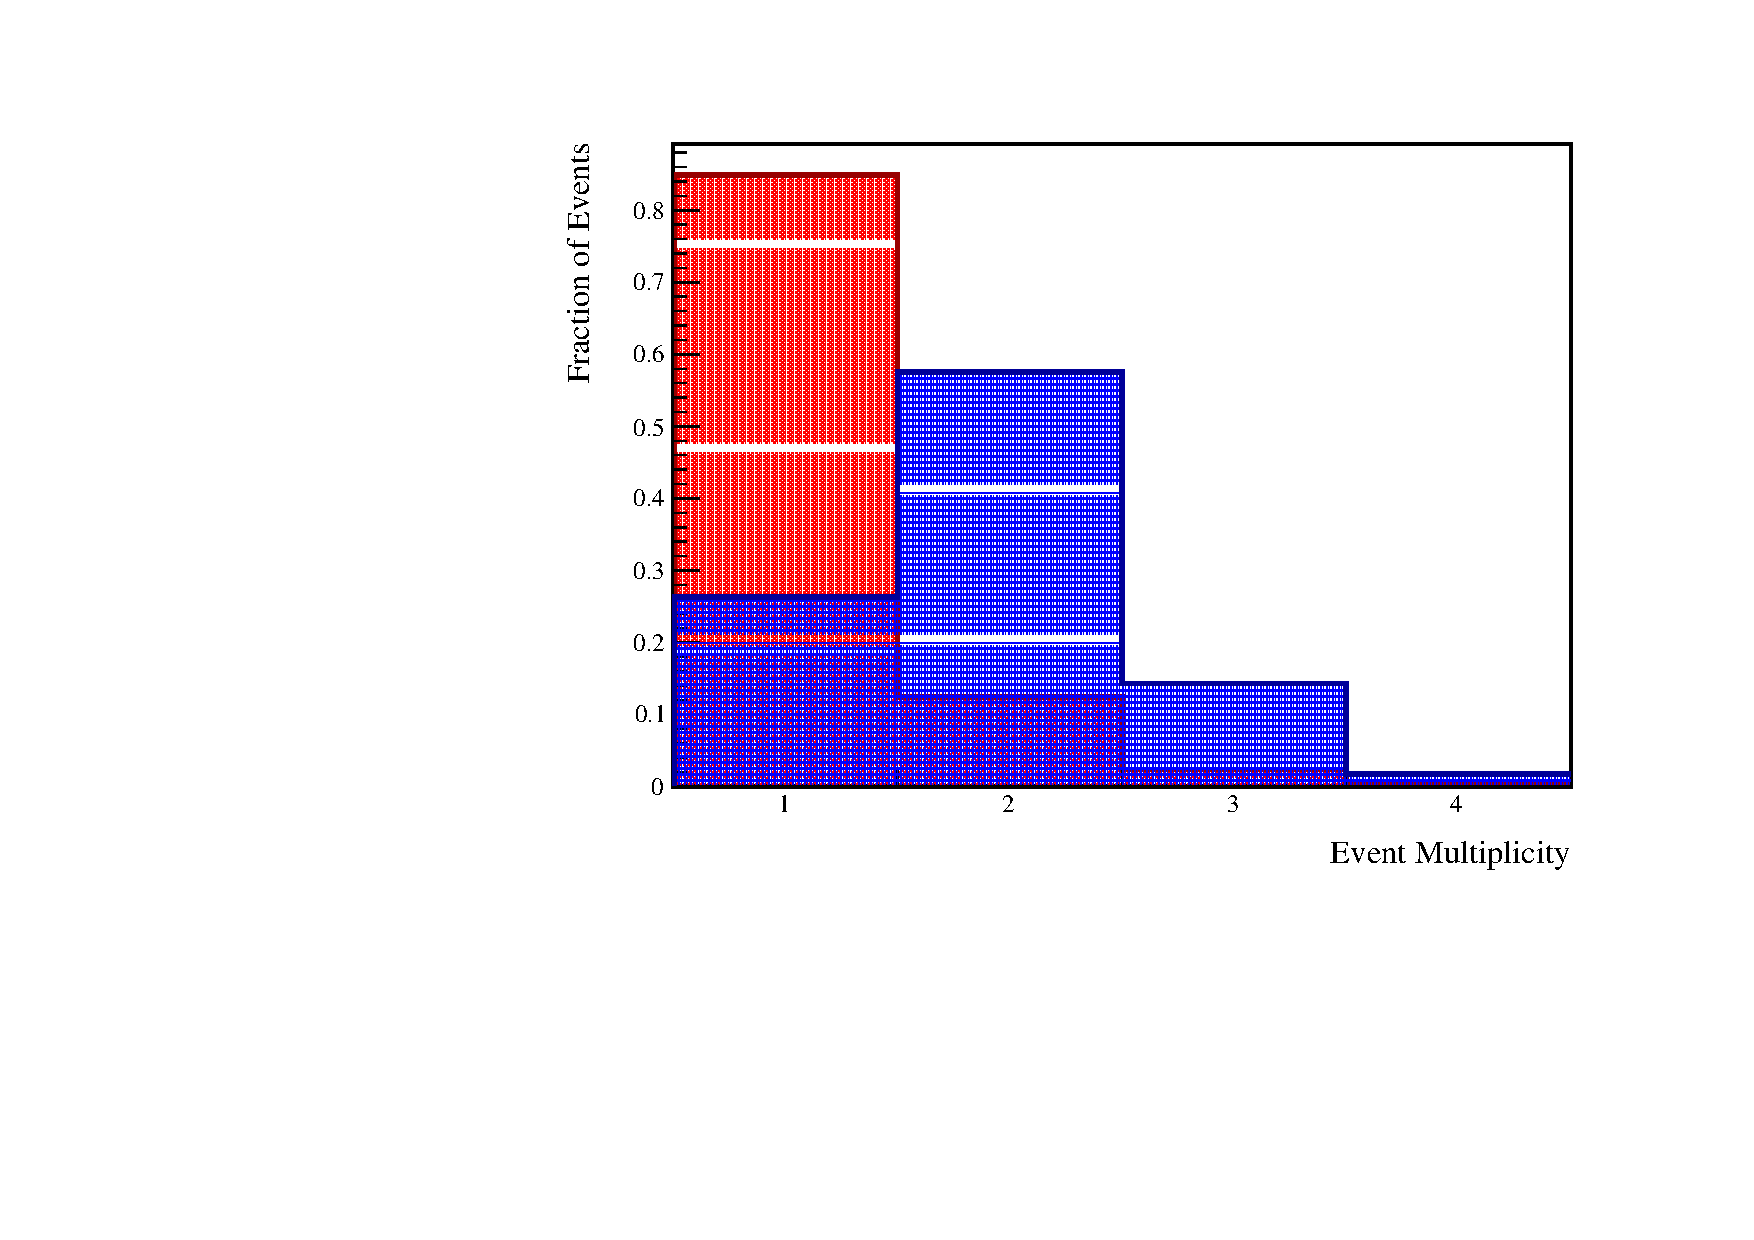
\includegraphics[width=0.8\textwidth]{MultHist}
  \caption[Event Multiplicity in E.S. decay and BG model simulations]{\label{fig:multhist}
    The simulated distribution of ROI event multiplicities in the background model (red) and \bbes\ (blue) to \SP{0}{+}{1} decay. These simulations use the DS6 detector configuration.}
\end{figure}

\section{Simulation of Excited State Decays} \label{sec:essims}
Simulations of the \Ge{76} decay to excited states of \Se{76} are used to evaluate the detection efficiency of the analysis presented in this document.
Two different event generators are used to generate \Ge{76} \bb-decay\ within \Mage.
The first generator uses calculations of the phase space factors from J.~Kotila and F.~Iachello\cite{Kotila2012}.
It is implemented in the mage class \texttt{MGGeneratorDoubleBeta} using data tables with the distribution of both electron energies and angular correlations.
These data tables are provided for the \tnbb\ and \znbb\ decays to the ground state of \Se{76}, but not for the decays to any excited state of \Se{76}.
This calculation is an improvement over other phase space calculations thanks to an exact evalutation of the Dirac wave functions of the electrons involving a finite nuclear size and electron screening.

A second event generator packaged with \Mage\ is \texttt{DECAY0}\cite{Ponkratenko2000}, a FORTRAN program that generates a wide variety of $\beta\beta$- and $\beta$-decays.
\texttt{DECAY0} is capable of generating \tnbb\ and \znbb\ for \Ge{76} to \SP{0}{+}{} and \SP{2}{+}{} excited states of \Se{76} using a variety of physics mechanisms.
For the excited state decays, the deexcitation $\gamma$s and conversion electrons are also generated.
Several modifications were made to \texttt{DECAY0} for this analysis.
First, the precision of the excited state deexcitation energies was increased from 1~keV to 0.001~keV (The $\gamma$ energies changed from 559 to 559.101~keV, from 563 to 563.178~keV, from 657 to 657.041~keV, and from 1216 to 1216.104~keV).
Second, angular correlations were added for the \SP{2}{+}{2}-\SP{2}{+}{1}-\SP{0}{+}{g.s.} deexcitation $\gamma$ cascade which involves a 657~keV $\gamma$ with multipolarity E2+M1 and mixing ratio of $+5.2$ followed by a 559~keV $\gamma$ with multipolarity E2\cite{SINGH1995}.
The angular distribution between the $\gamma$s is\cite{Evans1955} 
\begin{equation}
  P(\theta)\propto 1-0.372\cdot\cos^2(\theta)+0.0439\cdot\cos^4(\theta)
\end{equation}
The angular correlation for the \SP{0}{+}{1}-\SP{2}{+}{1}-\SP{0}{+}{g.s.} deexcitation was already correctly included in \texttt{DECAY0}, and is represented by the angular distribution\cite{SINGH1995, Evans1955}
\begin{equation}
  P(\theta)\propto 1-3\cdot\cos^2(\theta)+4\cdot\cos^4(\theta)
\end{equation}
Running \texttt{DECAY0} produces data files with the initial momenta of the generated particles.
The \Mage\ class \texttt{MGGeneratorDecay0} reads these datafiles and generates initial positions for these events.

\begin{figure}[h]
  \centering
  \includegraphics[width=.9\linewidth]{ESsim}
  \caption[Simulation of multiplicty 2 events from \tnbb\ to \SP{0}{+}{1}]{\label{fig:2dessim}
    Multiplicity 2 energy spectrum produced by a \texttt{DECAY0} simulation of \tnbb\ of \Ge{76} to the \SP{0}{+}{1} state of \Se{76}.
  }
\end{figure}
Simulations were run for \Ge{76} \tnbb\ and \znbb\ to the \SP{0}{+}{1}, \SP{2}{+}{1} and \SP{2}{+}{2} excited states of \Se{76} using the \texttt{DECAY0} generator.
For each decay mode, 5,000,000 event primaries were generated in the bulk of the enriched detectors and 500,000 primaries were generated in the bulk of the natural detectors.
These events were skimmed with the relative activities set equal to the total isotopic mass in each set of detectors: 26.2538~kg in enriched detectors, and 1.1232~kg in natural detectors.
These simulations were additionally post-processed and skim files were produced both with and without a dead layer, and with and without dead times.
Figure~\ref{fig:2dessim} shows an energy spectrum of multiplicity~2 events produced by the simulation of the \Ge{76} decay to the \SP{0}{+}{1} excited state of \Se{76}.

\subsection{Comparing \texttt{DECAY0} to the Kotila and Iachello generator} \label{sec:decay0vskandi}
\begin{figure}
  \centering
  \subfloat{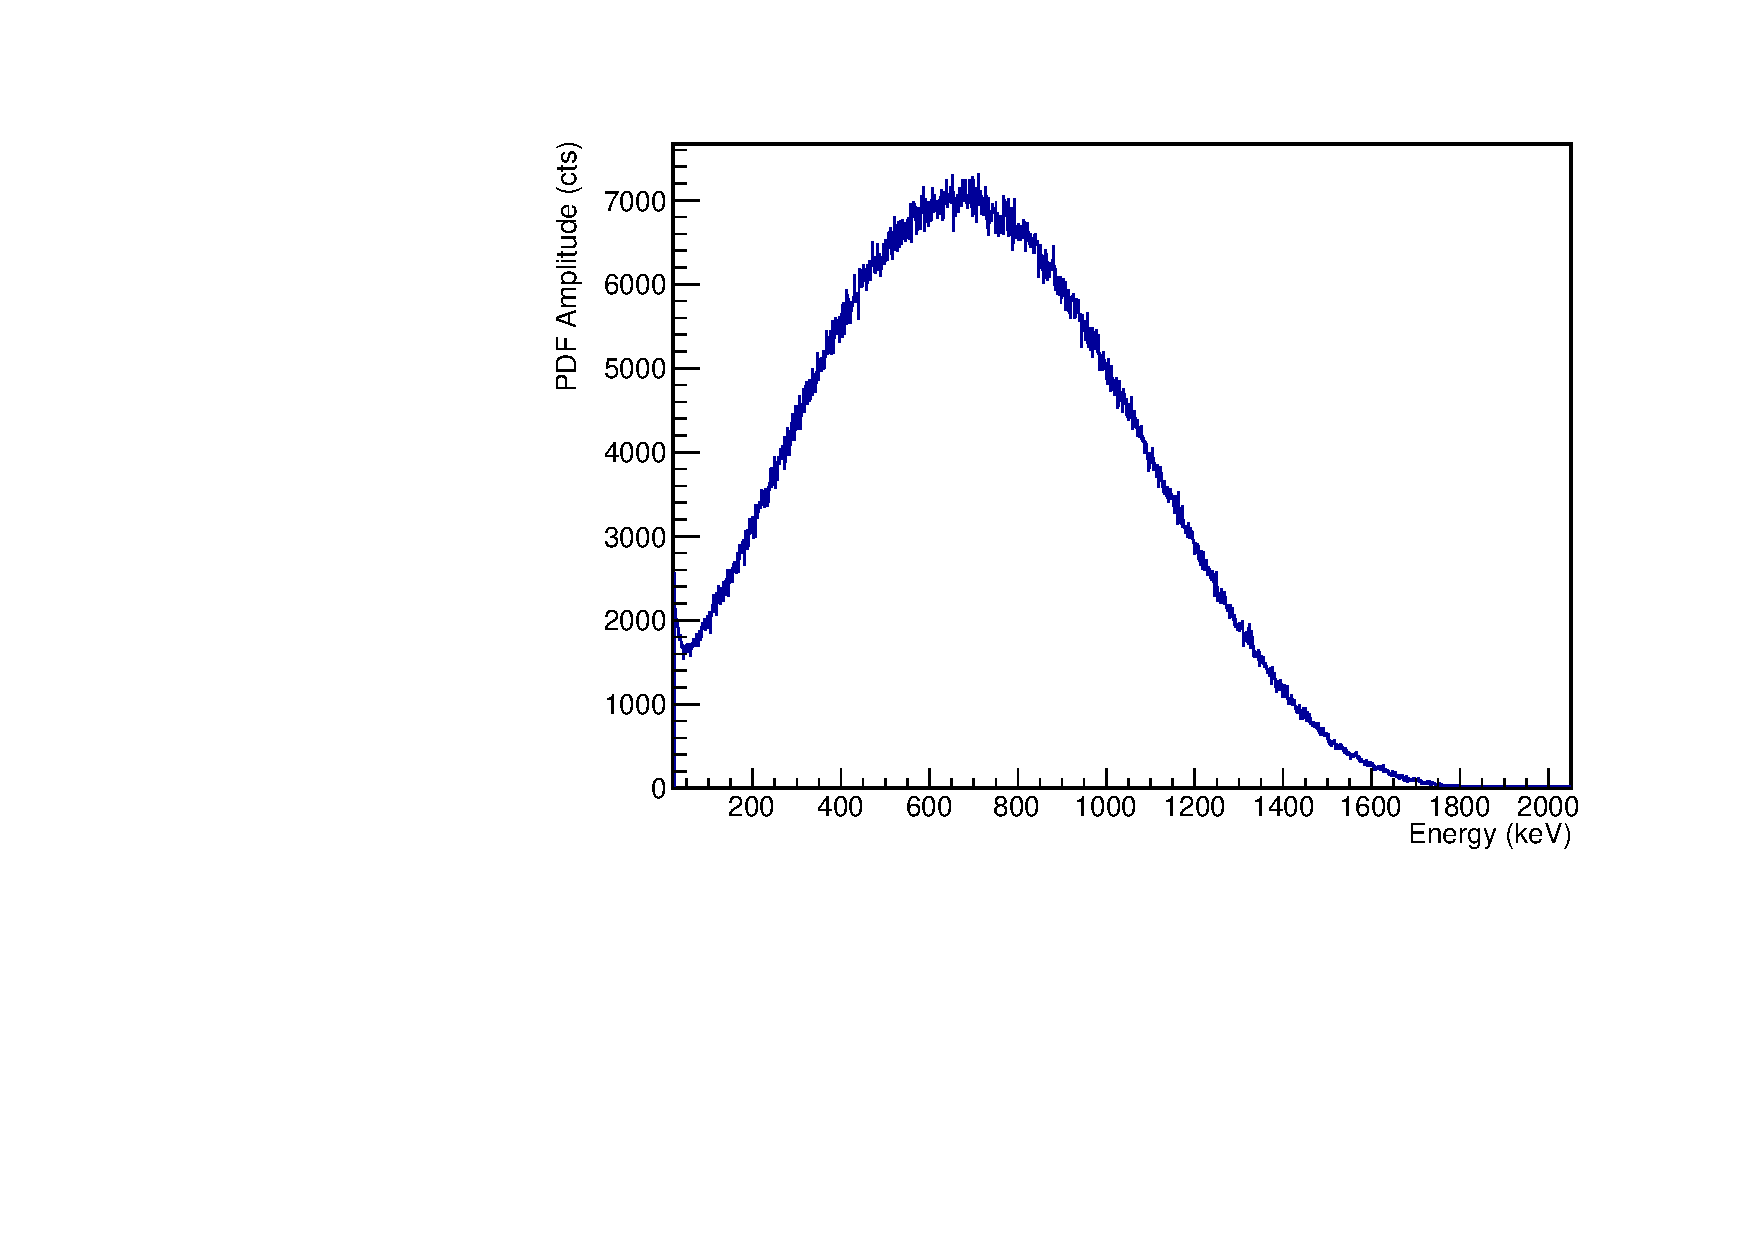
\includegraphics[width=0.5\linewidth]{decay0gsspectrum}}
  \subfloat{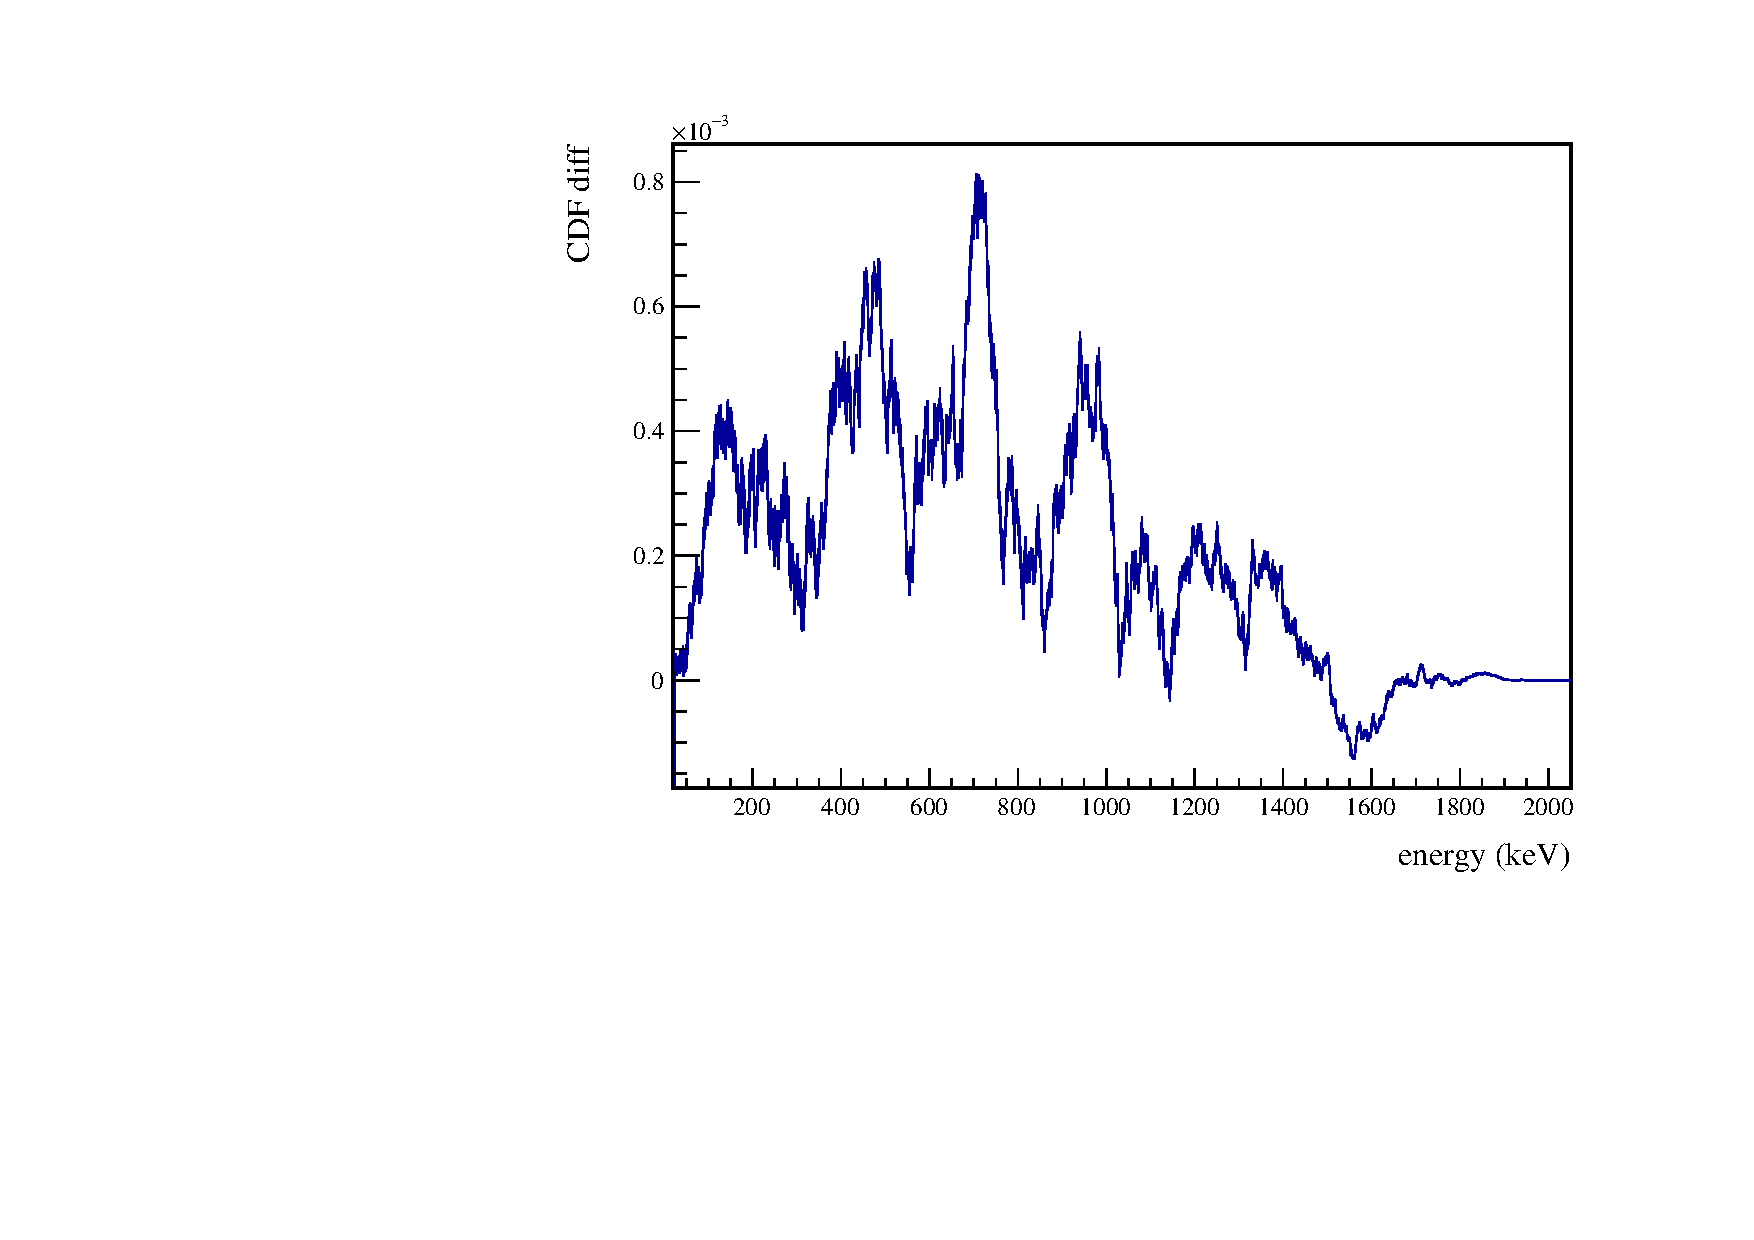
\includegraphics[width=0.5\linewidth]{decay0KS}}
  \caption[KS test comparing \texttt{decay0} to Kotila and Iachello \tnbb\ to g.s. spectra]{\label{fig:kstest}
    A KS test is performed comparing the \texttt{DECAY0} \tnbb\ to the ground state energy spectrum to that of Kotila and Iachello. The \texttt{decay0} spectrum is shown, along with the difference between the CDF of each spectrum.
  }
\end{figure}
The Kotila and Iachello generator performs a more accurate calculation of phase space than \texttt{DECAY0} and is used for the \MJD 's measurement of \tnbb\ and \znbb\ to the ground state.
Because Kotila and Iachello present only the phase space integral for the excited state decays, and do not include the energy and angular distributions, \texttt{DECAY0} is used for this analysis.
To evaluate the accuracy of \texttt{DECAY0}, we can compare the spectrum of the \tnbb\ to the ground state it generates to that of Kotila and Iachello; this comparison will reflect the error with respect to the true value if we assume that the errors corrected by Kotila and Iachello are the dominant errors in \texttt{DECAY0}.
This comparison is performed using a Kolmogorov-Smirnov (KS) test.
The KS test statistic is the maximum difference between the CDF of each normalized energy spectrum.
As we will see in Section~\ref{sec:MSenergycuts}, this test is useful in evaluating the uncertainties in the measurement presented in this document.
The CDF difference is shown in Figure~\ref{fig:kstest}, with a KS statistic of 0.00081.
While this error is statistically significant at a level of 97\%, we will see that the systematic error generated is subdominant.

\section{Background Model Simulation}
A simulation of the background spectrum measured by the \MJD\ will be used to optimize the search for \bbes.
\Mage\ simulations of a variety of decay chains, including \Th{232}, \iso{238}{U}, \iso{40}{K}, \Co{60}, \iso{222}{Rn} and \Ge{68}, have been run using event generators internal to \geant.
A large number of component groups have been defined, encompassing one or more physical components of the experiment (e.g.~all signal electronic connectors are a single component group).
The event generators use the combined geometries of these groups to generate start positions, which can be in either the bulk of a component group, or on the surface.
The activity of each isotope from each component group is determined by fitting a linear combination of the simulated energy spectra to the measured background spectrum.
An incomplete version of this fit is used for this document, producing the spectra in Figures~\ref{fig:bgsim1D} and~\ref{fig:bgsim2D}\cite{buuck2019}.
\Ge{68} decays with a half-life of 271~days, so its activity is scaled to represent the exposure-weighted activity of each major dataset.
\iso{210}{Pb} in the lead shield is simulated using a special generator that samples bremsstrahlung x-rays emitted from the surface of a thick lead shield \cite{VOJTYLA1996}.

\begin{figure}
  \centering
  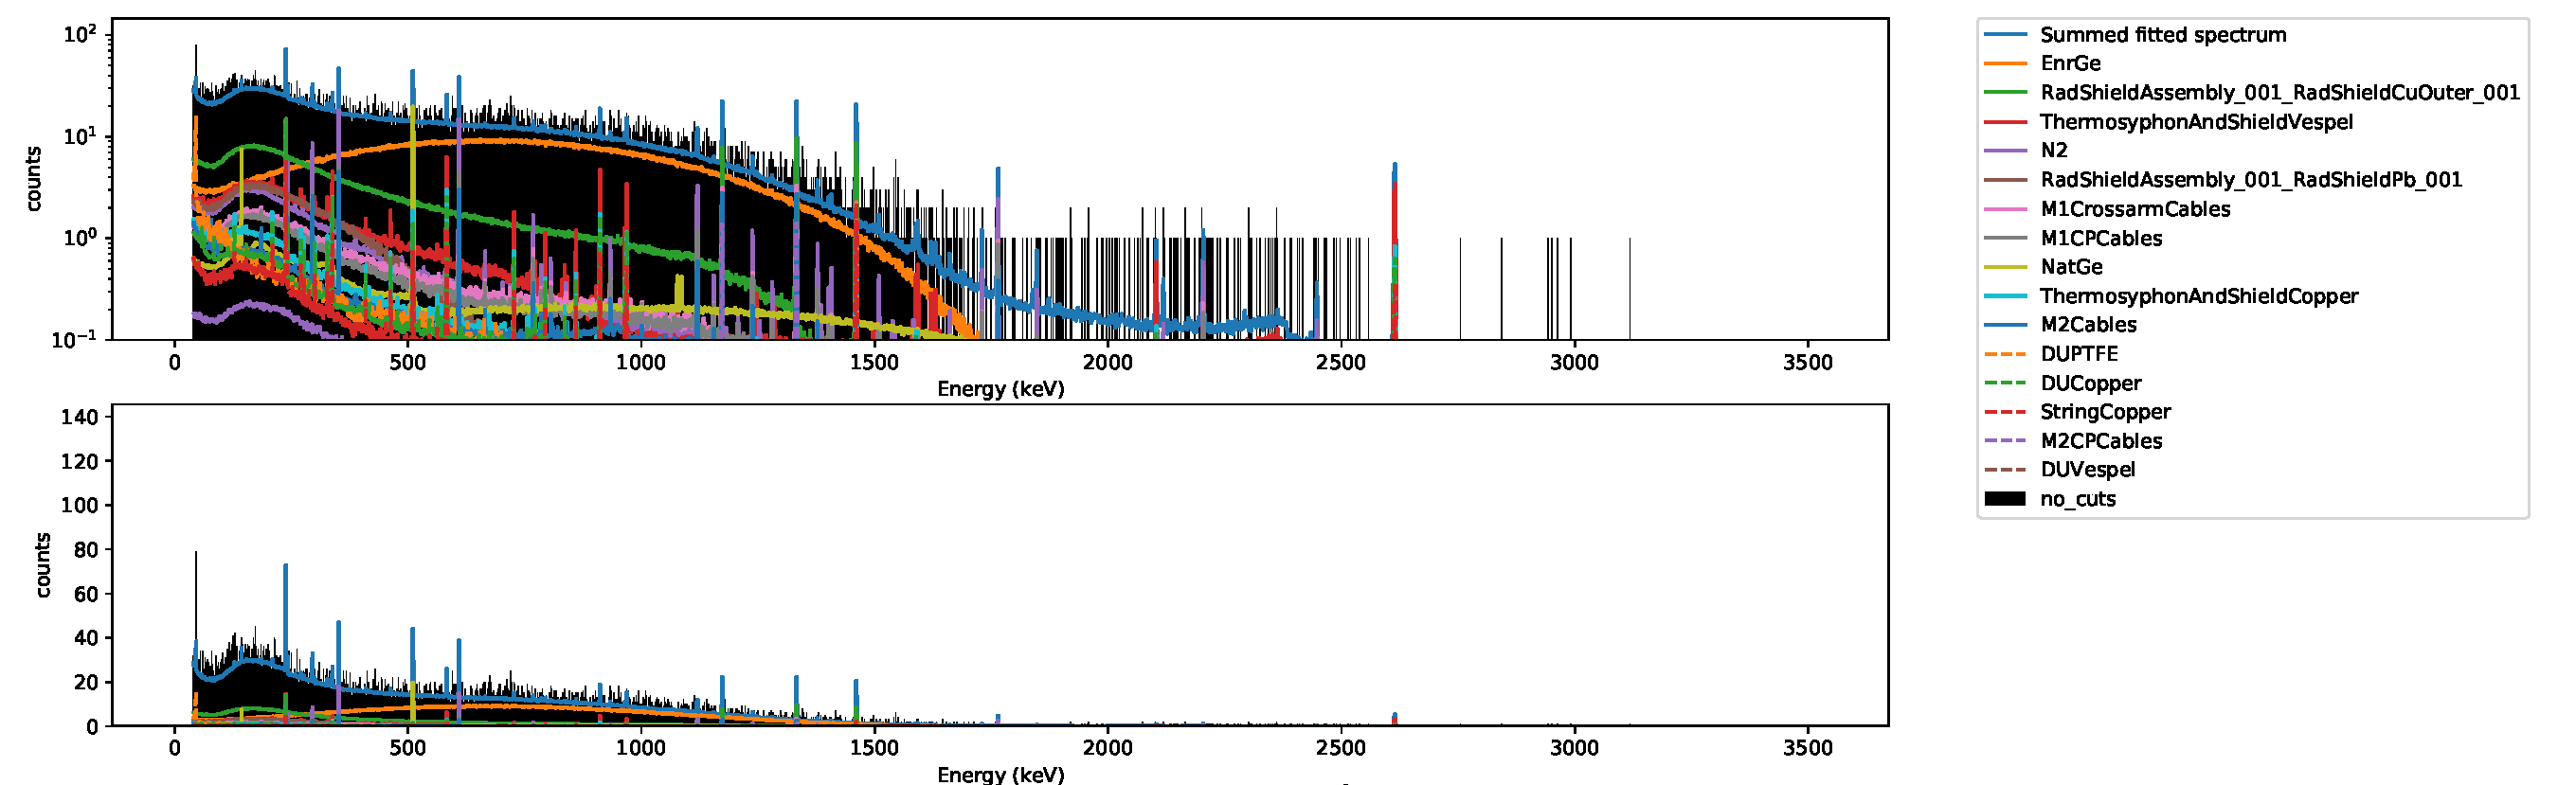
\includegraphics[width=1\linewidth]{BGsim1D}
  \caption[Simulation of multiplicty 1 events from the background model]{\label{fig:bgsim1D}
    Energy spectrum of observed multiplicity 1 events produced from a simulation of the preliminary background model, with the highest contributing components labelled.
  }
\end{figure}

\begin{figure}
  \centering
  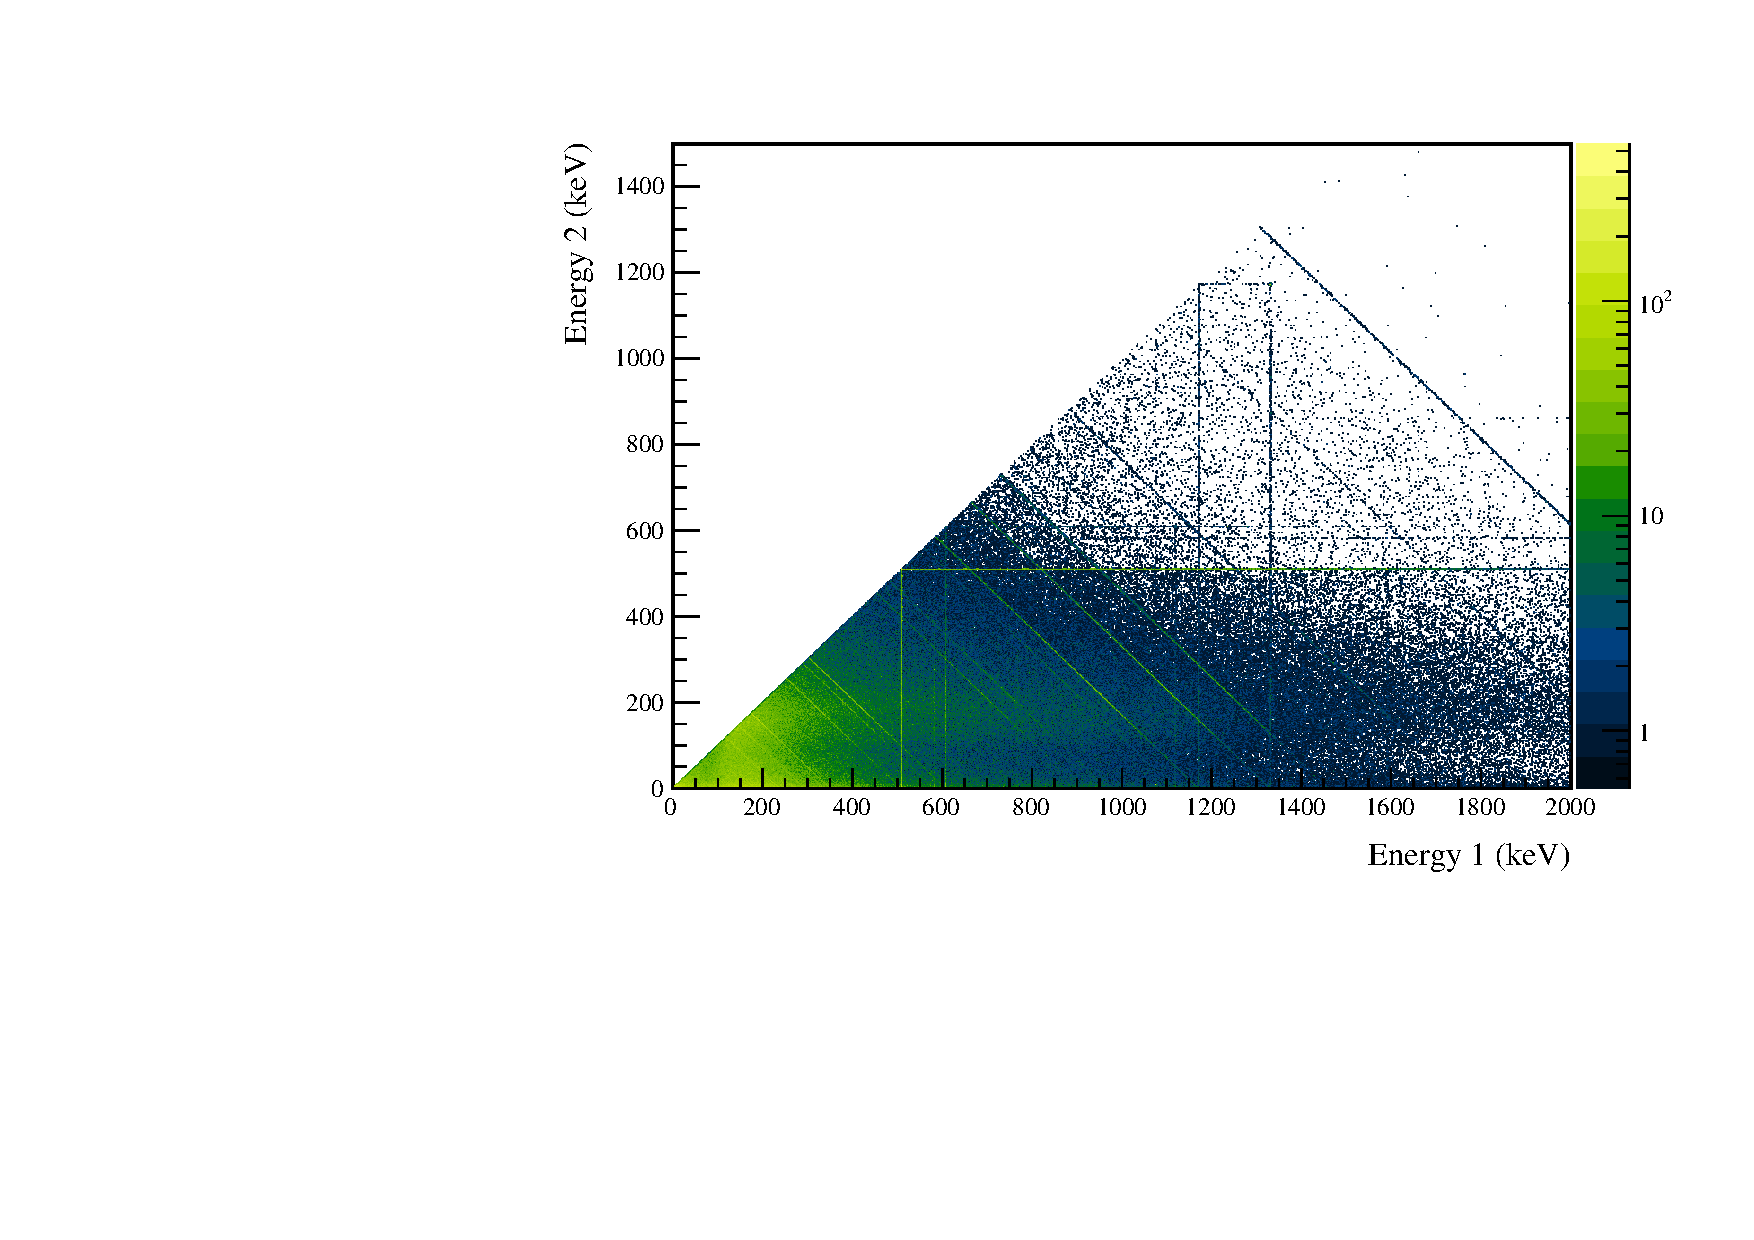
\includegraphics[width=.9\linewidth]{BGsim2D}
  \caption[Simulation of multiplicty 2 events from the background model]{ \label{fig:bgsim2D}
    Multiplicity 2 energy spectrum produced by a simulation of a preliminary version of the \MJD\ background model.
  }
\end{figure}
The background model used for this analysis is known to be inaccurate.
Since it is only used for optimizing the search for \bbes\ and is not important for the detection efficiency calculation, this does not affect the accuracy of the result presented.
For future versions of this analysis, a complete and more accurate background model will be used, which should result in small improvements to the cut optimization.

\section{\Co{56} Simulation} \label{sec:calsims}
Calibration of the \MJD\ is performed for each module using a line source that is injected by motor into a spiral track that winds around the module.
Simulations of the \Co{56} calibration sources are performed using the \geant\ generators for these isotopes, and a spiral position sampler written in \Mage.
The detection efficiency test described in Section~\ref{sec:Co56} uses the \Co{56} source simulation.
The simulated spectra for the \Co{56} source can be seen in Figures~\ref{fig:56Co1D} and~\ref{fig:Co56Sim2D}
\begin{figure}
  \centering
  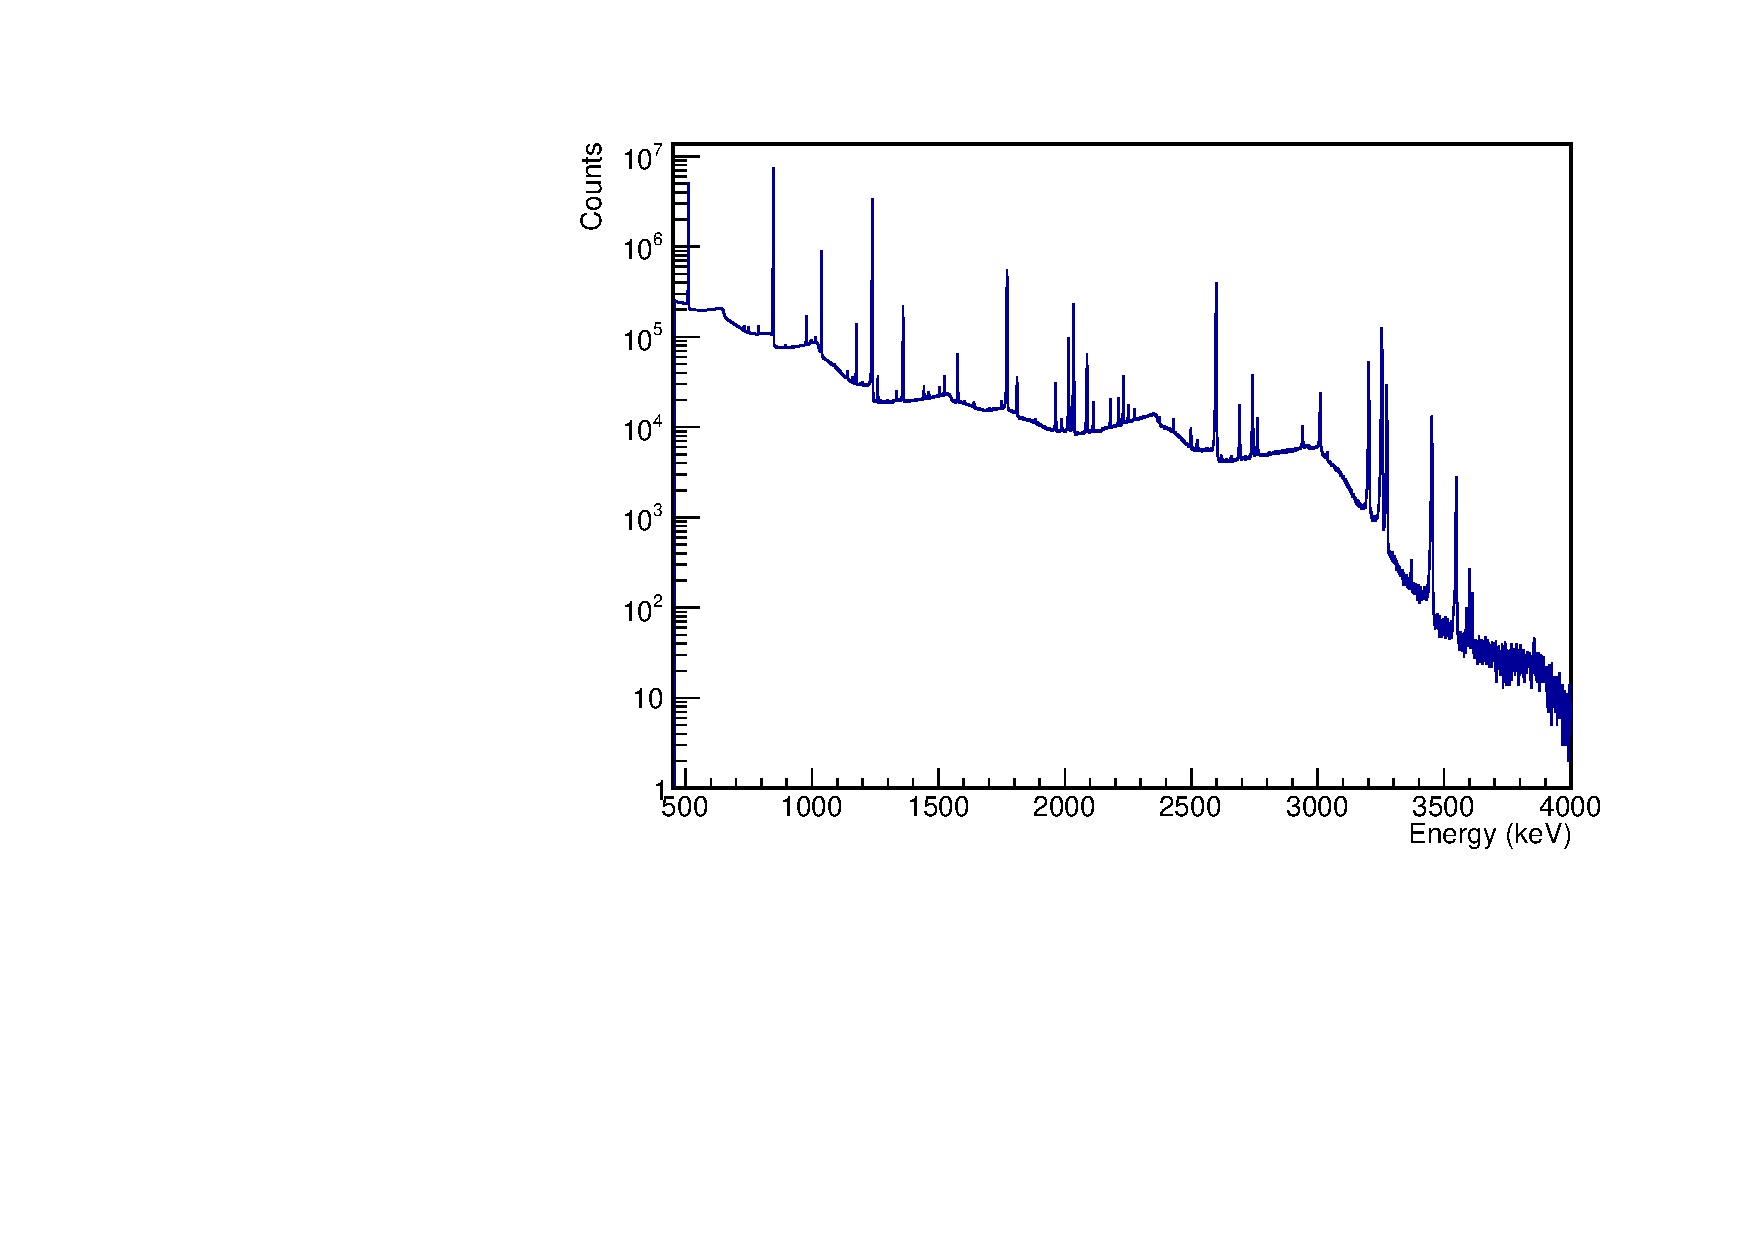
\includegraphics[width=.8\linewidth]{Co56Sim1D}
  \caption[Simulation of multiplicty 1 events from \Co{56} line source]{ \label{fig:56Co1D}
    Energy spectrum of multiplicity 1 events produced from a simulation of the \Co{56} line source inserted into the module~1 calibration track.
  }
\end{figure}

\begin{figure}
  \centering
  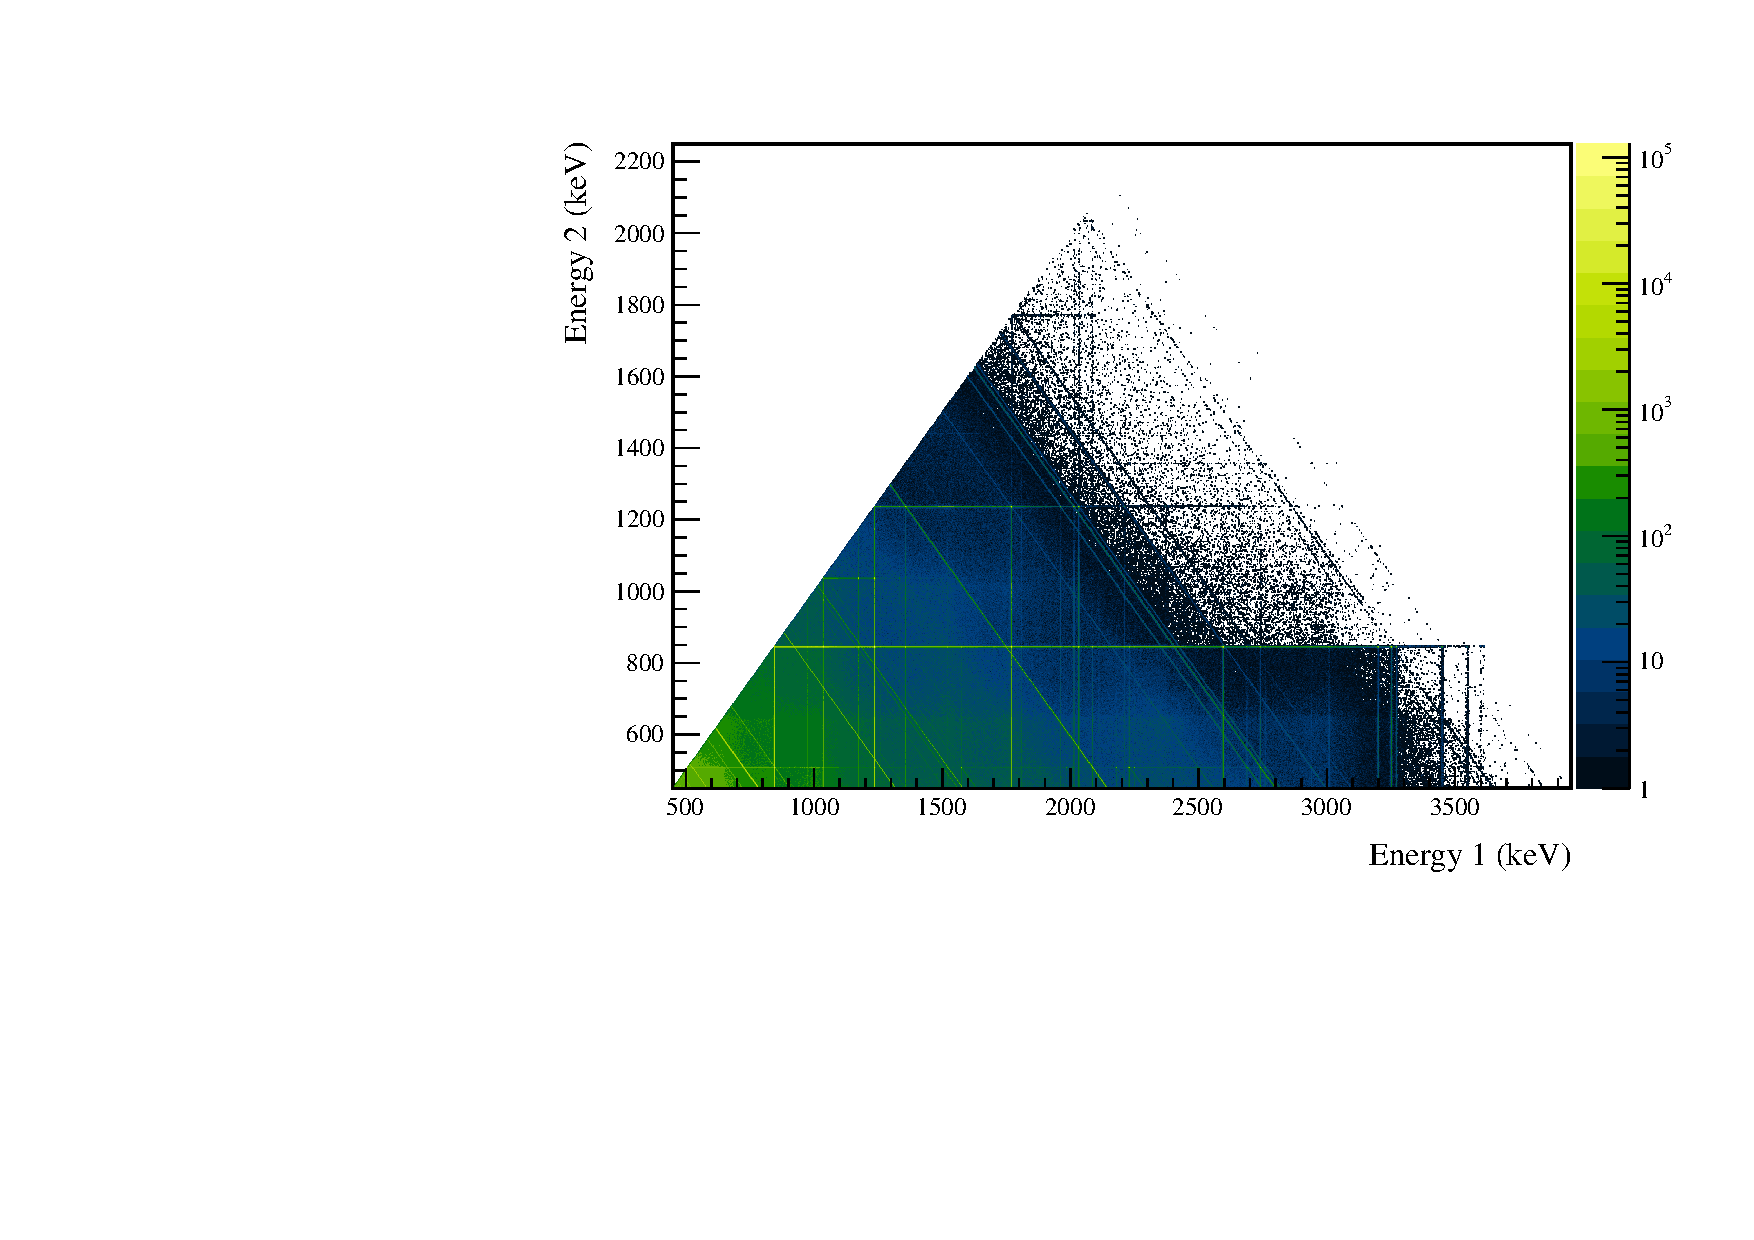
\includegraphics[width=.8\linewidth]{Co56Sim2D}
  \caption[Simulation of multiplicty 2 events from \Co{56} line source]{ \label{fig:Co56Sim2D}
    Multiplicity 2 energy spectrum produced by a simulation of the \Co{56} line source inserted into the module~1 calibration track.
  }
\end{figure}


\section{Simulation Skimming} \label{sec:simskim}
Skim files are produced containing parameters of interest from the post-processed files using the software \texttt{es\_skimsims}.
Skim files can also mix postprocessed files from multiple sources in ratios corresponding to the various activities of the sources.
\texttt{es\_skimsims} accepts as input a JSON file listing the simulated sources, the desired activity of each source, and the number of available event primaries.
From this, it calculates the number of primaries to accept from each source by maximizing the total number of events used while maintaining the correct ratio according to the activities.
Once this is done, it goes through each source sequentially and saves parameters of interest, including energy and detector position, to a \texttt{TTree}\cite{rootcern}.
As will be discussed in future chapters, single detector events are of little interest to this analysis, so only multi-detector events are recorded in order to maintain a small file size.
Multiplicity~1 events are recorded separately to a histogram according only to energy.
The skimming process also accounts for which sets of detectors are enabled.
Another input of \texttt{es\_skimsims} is a JSON file containing a list of detector configurations, containing a bitmask describing which detectors are and are not enabled.
The detector configurations will be discussed further in Section~\ref{sec:sds}.
When the skimmer encounters a disabled detector in an event, it ignores that detector, and does not count it towards the event multiplicity.
 
Each detector spends some portion of operating time dead, due to the finite rate at which the digitizers can retrigger, which typically cause $<0.1\%$ of HPGe hits to fail to read.
However, during early datasets, some detector channels were effected by a bug in the Gretina cards that caused a high rate of triggers on negative-energy noise pulses, resulting in much higher dead time fractions.
This effect is assumed to be random and uncorrelated between detectors.
The dead time of each detector is measured by counting the number of pulser events in each detector for each run.
Because the pulses occur at a fixed rate, we can predict the number of pulser events that should occur in any given run; the fraction of pulser events missed is assumed to represent the dead time fraction.
The JSON detector configuration file contains the dead time fraction and the statistical uncertainty (assuming binomial statistics with respect to the total number of expected pulser events) on that fraction for each active detector.
For each simulated detector hit, the data skimmer randomly throws out hits according to the probability represented by the dead fraction, treating that detector as inactive for that event.


\section{Selection of Multi-Detector Events}
Simultaneous detector hits are combined into events by the event builder.
Events are combined in a 4~$\mu$s rolling window.
This window is expected to accept virtually all true coincidence events (see Figure~\ref{fig:toffset}).
In a small number of runs, clocks between different Gretina cards were desynchronized.
For these runs, the clocks were resynchronized by applying a timing offset during event building that is measured by seeking the time offset that aligns pulser events.
With a typical overall rate between both modules of $<1$~Hz, $<0.4\%$ of all multi-site events are expected to originate from accidental coincidences, making this a negligible background.
Once all the data has gone through the standard \MJD\ processing chain, the skim files from all good open runs in datasets 1\-6a are collected into a single skim file containing a \texttt{TTree} with only multi-site events by the program \texttt{es\_skimdata}.

\begin{figure}[ht]
  \centering
  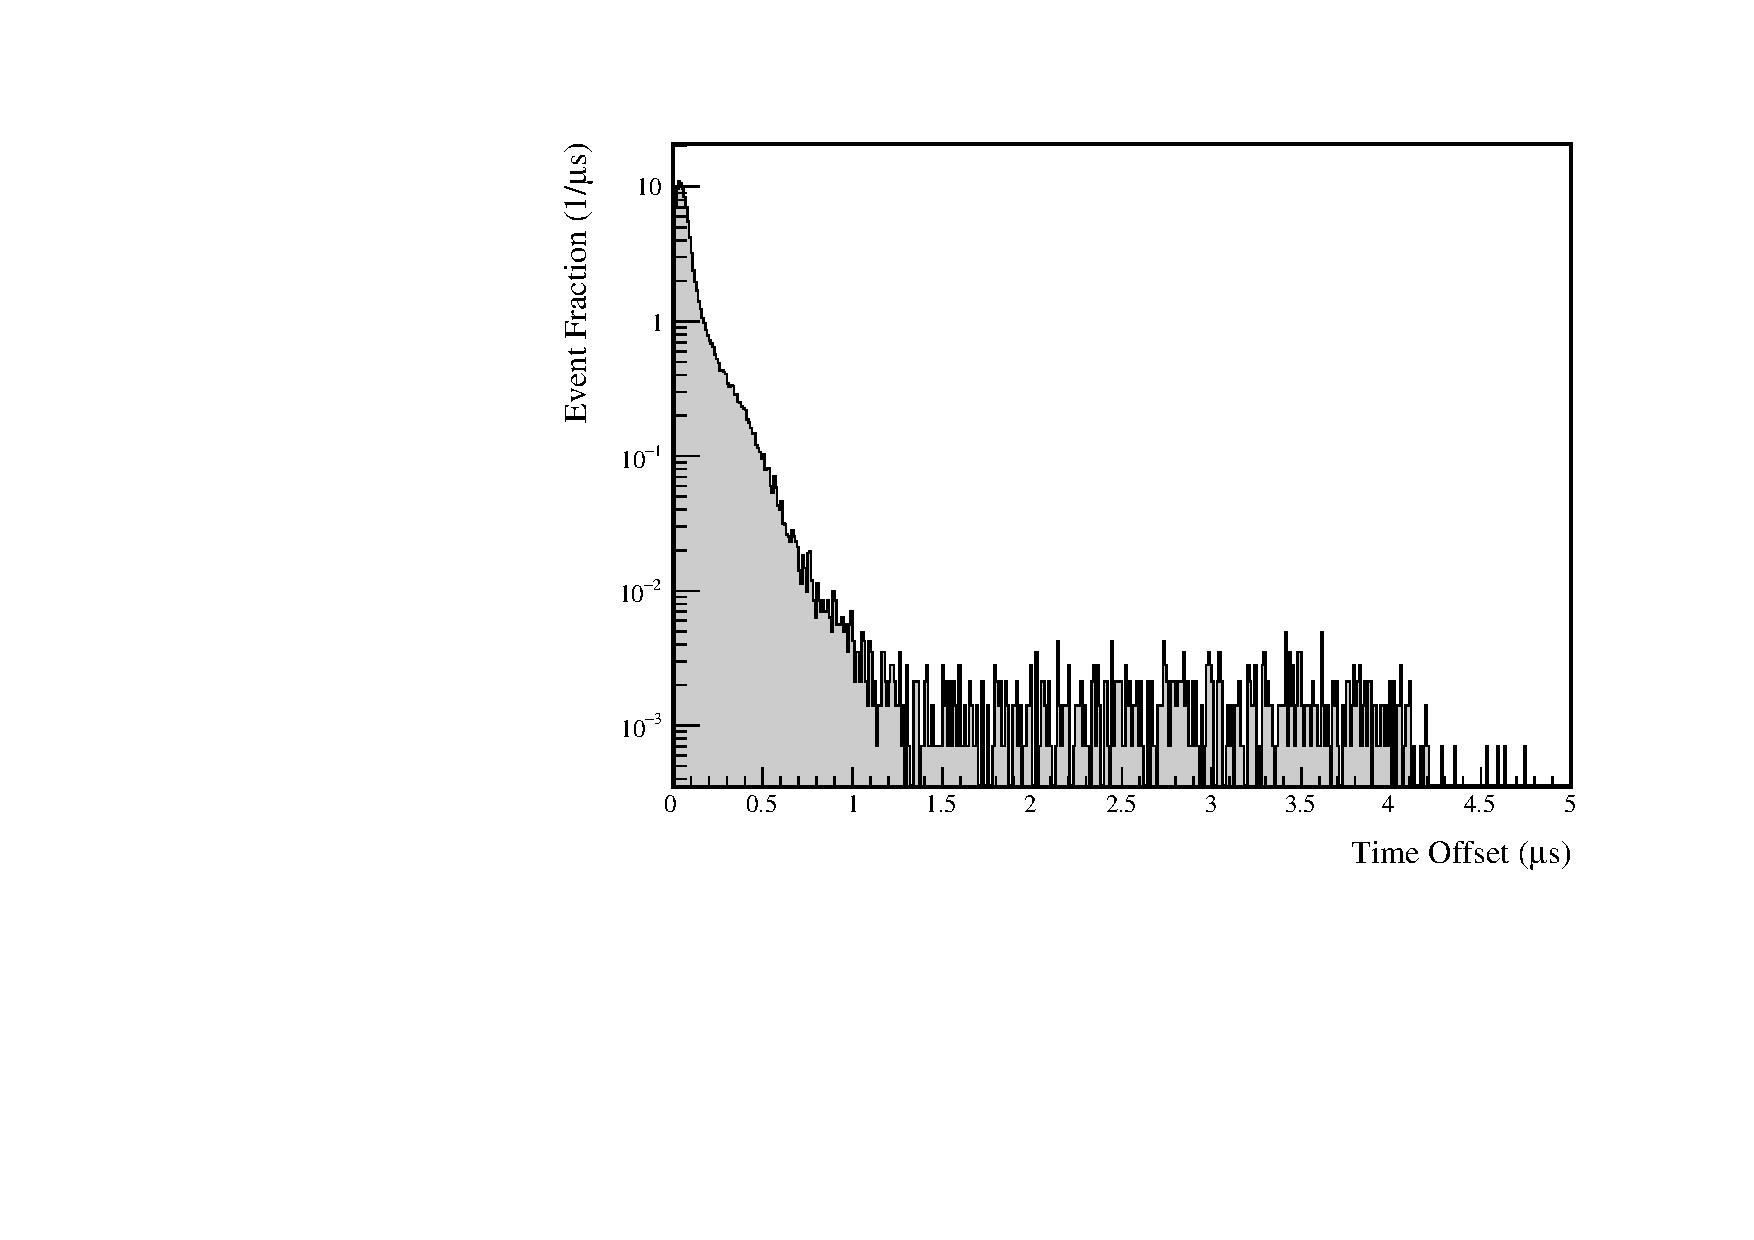
\includegraphics[width=0.8\textwidth]{toffset}
  \caption[Distribution of offset times within multi-detector events]{\label{fig:toffset}
    Distribution of time interval between individual hits within a multi-detector event during a \Th{228} calibration run. Offsets of greater than ${\sim}1.5$~$\mu$s are due to pileup, which is significant due to the high data rate of calibration runs. Offsets greater than ${\sim}4~\mu$s must involve events with more than two hits, due to the event builder time window.}
\end{figure}

\subsection{Variation in Detector Configuration} \label{sec:sds}
Throughout the runtime of the \MJD, not all detectors were simultaneously active, and within each dataset, the set of active detectors varied signficantly.
Because we are looking at \msmd\ events, the detection efficiency for \bbes\ events in any detector depends on which other detectors are enabled.
For this reason, detection efficiency is computed for each module in its entirety rather than for individual detectors.
To account for changes in detector configuration, each dataset is divided into subdatasets based on which detectors are active.
The subdatasets are described by a pair of 64-bit masks, one for each module, with each bit representing a single detector's state.
To decode the bitmask, the $b$'th least significant bit represents string position $P$, detector position $D$ if
\begin{equation}\label{eq:sdsbitmask}
  b = 8\cdot P + D
\end{equation}
The set of runs and active channels for each run were determined by the run selection and data cleaning committee, and the procedures are outlined in \cite{2018Reine}.
The program \texttt{es\_getdatasets} uses these selections to sort each run into a subdataset.

The detection efficiency is defined as the probability of a signal event in any detector, including inactive detectors.
Detection efficiency is calculated individually for each subdataset and for each module by creating a separate skim file for each subdataset as outlined in Section~\ref{sec:simskim}.
The final efficiency is then computed as an isotopic exposure weighted average of the efficiency within each subdataset.
Any efficiency uncertainties are assumed to be totally correlated between subdatasets.
The livetime of each subdataset is calculated by the program \texttt{es\_livetimes} by totalling the run time in each run, and subtracting any dead time that affects the entire module, including dead time caused by the muon veto system and by liquid nitrogen fills.
Additional sources of dead time that affect individual detectors are calculated as inefficiencies rather than being subtracted from the livetime, as discussed in Section~\ref{sec:simskim}.
This is done because dead time in any individual detector affects the detection efficiency of all other detectors.
The isotopic exposure is computed by multiplying the livetime of each module by the total isotopic mass in each module.
Since this includes mass in inactive detectors and dead layers, the isotopic exposure for this analysis will differ from that presented in the \znbb\ analysis.
Table~\ref{tab:subdatasets} lists each subdataset along with its livetime and exposure.

\begin{table}
  \caption[List of subdatasets, livetimes, efficiency and exposure]{\label{tab:subdatasets}
    List of each subdataset, labelled by the bitmasks defined in equation~\ref{eq:sdsbitmask}, with its livetime, detection efficiency measured for the \bbes\ to \SP{0}{+}{1} decay, and total isotopic exposure. Note the large amount of variance in the detection efficiency.
  }
  \scriptsize
  \begin{tabular}{|c|c c|c|c c|c c|c|}
  \hline
  DS & M1 Detector Mask & M2 Detector Mask & \makecell{Run Time\\(days)} & \makecell{M1 L.T.\\(days)} & M1 Eff. & \makecell{M2 L.T.\\(days)} & M2 Eff. & \makecell{Exposure\\(kg$\cdot$y)} \\
  \hline
  DS1 & 061a08001e0e1c00 & 0000000000000000 & 2.64 & 2.60 & 1.72\% & 0.00 & 0.00\% & 0.109 \\
  DS1 & 161a08341e0e1c00 & 0000000000000000 & 0.02 & 0.02 & 2.00\% & 0.00 & 0.00\% & 0.001 \\
  DS1 & 161a0c341e0e1c00 & 0000000000000000 & 4.51 & 4.48 & 1.94\% & 0.00 & 0.00\% & 0.188 \\
  DS1 & 161a0c361e0e1c00 & 0000000000000000 & 3.49 & 3.48 & 1.47\% & 0.00 & 0.00\% & 0.146 \\
  DS1 & 1e1a00001e0e1c00 & 0000000000000000 & 7.82 & 7.73 & 2.04\% & 0.00 & 0.00\% & 0.324 \\
  DS1 & 1e1a08001e0e1c00 & 0000000000000000 & 37.30 & 36.87 & 2.23\% & 0.00 & 0.00\% & 1.547 \\
  DS1 & 1e1a08041e0e1c00 & 0000000000000000 & 6.26 & 6.19 & 2.30\% & 0.00 & 0.00\% & 0.260 \\
  DS1 & 1e1a08141e0e1c00 & 0000000000000000 & 0.26 & 0.25 & 2.32\% & 0.00 & 0.00\% & 0.011 \\
  DS1 & 1e1a08301e0e1c00 & 0000000000000000 & 1.40 & 1.37 & 2.33\% & 0.00 & 0.00\% & 0.057 \\
  DS1 & 1e1a08341e0e1c00 & 0000000000000000 & 7.58 & 7.50 & 2.12\% & 0.00 & 0.00\% & 0.315 \\
  DS1 & 1e1a0c001e0e1c00 & 0000000000000000 & 2.83 & 2.78 & 2.25\% & 0.00 & 0.00\% & 0.117 \\
  DS1 & 1e1a0c041e0e1c00 & 0000000000000000 & 0.04 & 0.04 & 2.24\% & 0.00 & 0.00\% & 0.002 \\
  DS1 & 1e1a0c341e0e1c00 & 0000000000000000 & 0.67 & 0.67 & 2.32\% & 0.00 & 0.00\% & 0.028 \\
  DS2 & 1e1a08001e0e1c00 & 0000000000000000 & 38.92 & 38.52 & 2.28\% & 0.00 & 0.00\% & 1.617 \\
  DS2 & 1e1a0c001e0e1c00 & 0000000000000000 & 1.22 & 1.19 & 2.27\% & 0.00 & 0.00\% & 0.050 \\
  DS3 & 1e1a0c3e1e0e1c00 & 0000000000000000 & 29.88 & 29.67 & 2.64\% & 0.00 & 0.00\% & 1.245 \\
  DS4 & 0000000000000000 & 1c061a16060e1e00 & 19.15 & 0.00 & 0.00\% & 18.85 & 1.89\% & 0.622 \\
  DS5a & 08000020040e1c00 & 18060a02040e1e00 & 1.49 & 1.48 & 0.72\% & 1.46 & 1.16\% & 0.110 \\
  DS5a & 08080020040e1c00 & 18060a16060e1e00 & 2.51 & 2.49 & 0.86\% & 2.47 & 1.56\% & 0.186 \\
  DS5a & 08080030040e1c00 & 18060a02040e1e00 & 0.01 & 0.01 & 0.91\% & 0.01 & 1.14\% & 0.001 \\
  DS5a & 0e1a04321e0e1c00 & 08020a16060e1e00 & 2.69 & 2.71 & 2.33\% & 2.66 & 1.23\% & 0.201 \\
  DS5a & 0e1a0c321e0e1c00 & 0000000000000000 & 0.65 & 0.63 & 2.59\% & 0.00 & 0.00\% & 0.026 \\
  DS5a & 0e1a0c321e0e1c00 & 08060a16060e1e00 & 1.24 & 1.24 & 2.58\% & 1.21 & 1.52\% & 0.092 \\
  DS5a & 0e1a0c321e0e1c00 & 18060a02040e1e00 & 2.94 & 2.92 & 2.35\% & 2.89 & 1.15\% & 0.218 \\
  DS5a & 0e1a0c321e0e1c00 & 18060a1406061600 & 0.04 & 0.04 & 2.56\% & 0.04 & 0.95\% & 0.003 \\
  DS5a & 0e1a0c321e0e1c00 & 18060a1606060600 & 3.19 & 3.15 & 2.52\% & 3.16 & 0.82\% & 0.237 \\
  DS5a & 0e1a0c321e0e1c00 & 18060a16060e0600 & 3.30 & 3.28 & 2.53\% & 3.29 & 0.84\% & 0.246 \\
  DS5a & 0e1a0c3e1e0e1c00 & 1806020606081800 & 1.75 & 1.73 & 2.80\% & 1.73 & 0.76\% & 0.129 \\
  DS5a & 0e1a0c3e1e0e1c00 & 18060216060c1c00 & 6.84 & 6.77 & 2.80\% & 6.74 & 1.12\% & 0.507 \\
  DS5a & 0e1a0c3e1e0e1c00 & 18060216060e1e00 & 13.48 & 13.30 & 2.77\% & 13.27 & 1.26\% & 0.996 \\
  DS5a & 0e1a0c3e1e0e1c00 & 18060816060e1c00 & 0.05 & 0.05 & 2.59\% & 0.05 & 1.30\% & 0.004 \\
  DS5a & 0e1a0c3e1e0e1c00 & 18060a0606060c00 & 2.16 & 2.12 & 2.77\% & 2.12 & 1.02\% & 0.159 \\
  DS5a & 0e1a0c3e1e0e1c00 & 18060a16040e1e00 & 0.76 & 0.76 & 2.76\% & 0.74 & 1.29\% & 0.056 \\
  DS5a & 0e1a0c3e1e0e1c00 & 18060a1606060c00 & 0.25 & 0.25 & 2.78\% & 0.25 & 1.11\% & 0.019 \\
  DS5a & 0e1a0c3e1e0e1c00 & 18060a1606061800 & 1.88 & 1.86 & 2.78\% & 1.86 & 1.04\% & 0.140 \\
  DS5a & 0e1a0c3e1e0e1c00 & 18060a1606061c00 & 9.20 & 9.13 & 2.75\% & 9.06 & 1.41\% & 0.682 \\
  DS5a & 0e1a0c3e1e0e1c00 & 18060a16060c1c00 & 7.89 & 7.79 & 2.78\% & 7.79 & 1.41\% & 0.584 \\
  DS5a & 0e1a0c3e1e0e1c00 & 18060a16060e1c00 & 11.68 & 11.53 & 2.43\% & 11.51 & 1.42\% & 0.864 \\
  DS5a & 0e1a0c3e1e0e1c00 & 18060a16060e1e00 & 5.21 & 5.15 & 2.76\% & 5.13 & 1.56\% & 0.386 \\
  DS5a & 0e1a0c3e1e0e1c00 & 18061216060e1e00 & 2.39 & 2.37 & 2.77\% & 2.37 & 1.34\% & 0.178 \\
  DS5b & 1e1a0c3e1e0c1c00 & 18061216060e1e00 & 24.46 & 24.09 & 2.75\% & 24.06 & 1.34\% & 1.805 \\
  DS5b & 1e1a0c3e1e0c1c00 & 18061a16060e1e00 & 0.75 & 0.75 & 2.75\% & 0.75 & 1.73\% & 0.056 \\
  DS5b & 1e1a0c3e1e0e1c00 & 18061216060e1e00 & 14.28 & 14.12 & 2.86\% & 14.07 & 1.24\% & 1.057 \\
  DS5c & 1e1a0c3e1e0c1c00 & 0000000000000000 & 0.67 & 0.67 & 2.65\% & 0.00 & 0.00\% & 0.028 \\
  DS5c & 1e1a0c3e1e0c1c00 & 00060216060e0e00 & 0.78 & 0.76 & 2.65\% & 0.78 & 0.84\% & 0.058 \\
  DS5c & 1e1a0c3e1e0c1c00 & 00060a16060e0e00 & 5.91 & 5.82 & 2.75\% & 5.83 & 1.07\% & 0.437 \\
  DS5c & 1e1a0c3e1e0c1c00 & 00061216060e0e00 & 38.85 & 38.45 & 2.73\% & 38.29 & 0.91\% & 2.877 \\
  DS6a & 12000000000c0800 & 1002020006040e00 & 4.94 & 4.89 & 0.16\% & 4.89 & 0.42\% & 0.366 \\
  DS6a & 12000c20000c1c00 & 18061216060c1e00 & 17.22 & 17.03 & 0.78\% & 17.03 & 1.13\% & 1.277 \\
  DS6a & 12020000040c0800 & 1802020006040e00 & 5.69 & 5.63 & 0.29\% & 5.62 & 0.50\% & 0.422 \\
  DS6a & 12020c00040c1800 & 1802020006040e00 & 7.90 & 7.79 & 0.68\% & 7.78 & 0.50\% & 0.584 \\
  DS6a & 12080c20000c1c00 & 18061216060c1e00 & 12.23 & 12.11 & 0.96\% & 12.09 & 1.13\% & 0.907 \\
  DS6a & 12120c3e1c0c1c00 & 18061216060c1e00 & 0.56 & 0.54 & 1.90\% & 0.56 & 1.10\% & 0.041 \\
  DS6a & 16020c10040c1800 & 1806020006060e00 & 14.89 & 14.73 & 0.90\% & 14.68 & 0.69\% & 1.103 \\
  DS6a & 160a0c321c0c1c00 & 1806021006061e00 & 5.87 & 5.80 & 2.05\% & 5.80 & 0.89\% & 0.435 \\
  DS6a & 1e0a0c321c0c1c00 & 0000000000000000 & 0.23 & 0.23 & 2.31\% & 0.00 & 0.00\% & 0.010 \\
  DS6a & 1e0a0c321c0c1c00 & 1806020006040200 & 10.00 & 9.89 & 2.31\% & 9.89 & 0.27\% & 0.741 \\
  DS6a & 1e0a0c321c0c1c00 & 1806020006040600 & 7.43 & 7.35 & 2.31\% & 7.32 & 0.41\% & 0.550 \\
  DS6a & 1e0a0c321c0c1c00 & 1806020006041600 & 4.88 & 4.83 & 2.31\% & 4.81 & 0.48\% & 0.362 \\
  DS6a & 1e0a0c321c0c1c00 & 1806021006061e00 & 6.11 & 6.05 & 2.31\% & 6.04 & 0.89\% & 0.453 \\
  DS6a & 1e120c3e1c0c1c00 & 18061216060c1e00 & 2.12 & 2.11 & 2.39\% & 2.09 & 1.13\% & 0.157 \\
  DS6a & 1e1a0c321c0c1c00 & 1806020006060e00 & 5.56 & 5.51 & 2.49\% & 5.53 & 0.69\% & 0.414 \\
  DS6a & 1e1a0c321c0c1c00 & 1806021006040e00 & 16.87 & 16.69 & 2.49\% & 16.64 & 0.69\% & 1.250 \\
  DS6a & 1e1a0c321c0c1c00 & 1806021006041e00 & 11.93 & 11.81 & 2.49\% & 11.79 & 0.86\% & 0.885 \\
  DS6a & 1e1a0c321c0c1c00 & 1806021006060e00 & 2.56 & 2.55 & 2.49\% & 2.55 & 0.73\% & 0.191 \\
  DS6a & 1e1a0c3a1c0c1c00 & 1806020006040e00 & 8.66 & 8.59 & 2.60\% & 8.59 & 0.65\% & 0.644 \\
  DS6a & 1e1a0c3a1c0c1c00 & 1806021006040e00 & 7.93 & 7.84 & 2.60\% & 7.83 & 0.69\% & 0.588 \\
  DS6a & 1e1a0c3a1c0c1c00 & 1806021006041e00 & 1.24 & 1.23 & 2.60\% & 1.23 & 0.86\% & 0.092 \\
  DS6a & 1e1a0c3e1c0c1c00 & 0000000000000000 & 0.06 & 0.05 & 2.69\% & 0.00 & 0.00\% & 0.002 \\
  DS6a & 1e1a0c3e1c0c1c00 & 1806000006040e00 & 7.85 & 7.81 & 2.69\% & 7.54 & 0.61\% & 0.577 \\
  DS6a & 1e1a0c3e1c0c1c00 & 1806020006041e00 & 5.96 & 5.88 & 2.65\% & 5.89 & 0.81\% & 0.441 \\
  DS6a & 1e1a0c3e1c0c1c00 & 1806021006041e00 & 3.56 & 3.52 & 2.69\% & 3.52 & 0.86\% & 0.264 \\
  DS6a & 1e1a0c3e1c0c1c00 & 18060210060c1e00 & 15.72 & 15.56 & 2.69\% & 15.51 & 0.92\% & 1.165 \\
  DS6a & 1e1a0c3e1c0c1c00 & 1806021206041e00 & 10.09 & 9.95 & 2.69\% & 9.97 & 0.89\% & 0.747 \\
  DS6a & 1e1a0c3e1c0c1c00 & 18060214060c0e00 & 5.65 & 5.60 & 2.69\% & 5.66 & 0.80\% & 0.422 \\
  DS6a & 1e1a0c3e1c0c1c00 & 18060214060c1e00 & 7.83 & 7.76 & 2.69\% & 7.74 & 0.98\% & 0.581 \\
  DS6a & 1e1a0c3e1c0c1c00 & 18060214060e1e00 & 58.28 & 57.56 & 2.67\% & 57.43 & 0.95\% & 4.311 \\
  DS6a & 1e1a0c3e1c0c1c00 & 1806121206041e00 & 1.00 & 0.98 & 2.69\% & 1.00 & 1.01\% & 0.074 \\
  DS6a & 1e1a0c3e1c0c1c00 & 18061212060c1e00 & 12.96 & 12.80 & 2.69\% & 12.80 & 1.07\% & 0.959 \\
  DS6a & 1e1a0c3e1c0c1c00 & 18061216060c1e00 & 26.05 & 25.76 & 2.69\% & 25.72 & 1.13\% & 1.930 \\
  \hline
  DSTotal & -- & -- & 621.97 & 615.24 & 2.35\% & 487.97 & 1.00\% & 41.923 \\
  \hline
\end{tabular}
\end{table}

\subsection{Dead Layer Effects} \label{sec:DL}
For multi-detector events, each individual hit may be degraded by the dead layer, so the loss of sensitivity from dead layers is larger for this search than for searches for single-site events.
For this reason, dead layer effects are treated as a loss of detection efficiency instead of a loss of exposure (as in the \znbb\ analysis).
Dead layers are included in the simulations as a part of simulation post-processing.
To account for uncertainty in the thickness of the dead layer, two separate simulations are run, with and without dead layers.
By comparing the efficiency measurement from each simulation, we measure the size of the dead layer effect.
The percent uncertainty in the efficiency loss from dead layers is assumed to be the same as the percent uncertainty in the dead layer thickness.
Typical loss of efficiency for multi-site peaks is 25-35\%; for the \tnbb\ to the \SP{0}{+}{1} decay, the losses are 26\% for module~1 and 34\% for module~2.
The uncertainty in the dead layer tends to be one of the dominant uncertainties in measuring the detection efficiency.
This is much larger than the ${\sim}10\%$ loss seen in the \znbb\ analysis for two reasons.
First, for multi-detector events, there are multiple hits that could possibly be lost to the dead layer.
Second, $\gamma$ hits will be more concentrated at the surface of the detectors, near the dead layers, than \bb\ sites.
The effect of dead layers on detection efficiency can be seen in Figure~\ref{fig:dldt}.

\begin{figure}
  \centering
  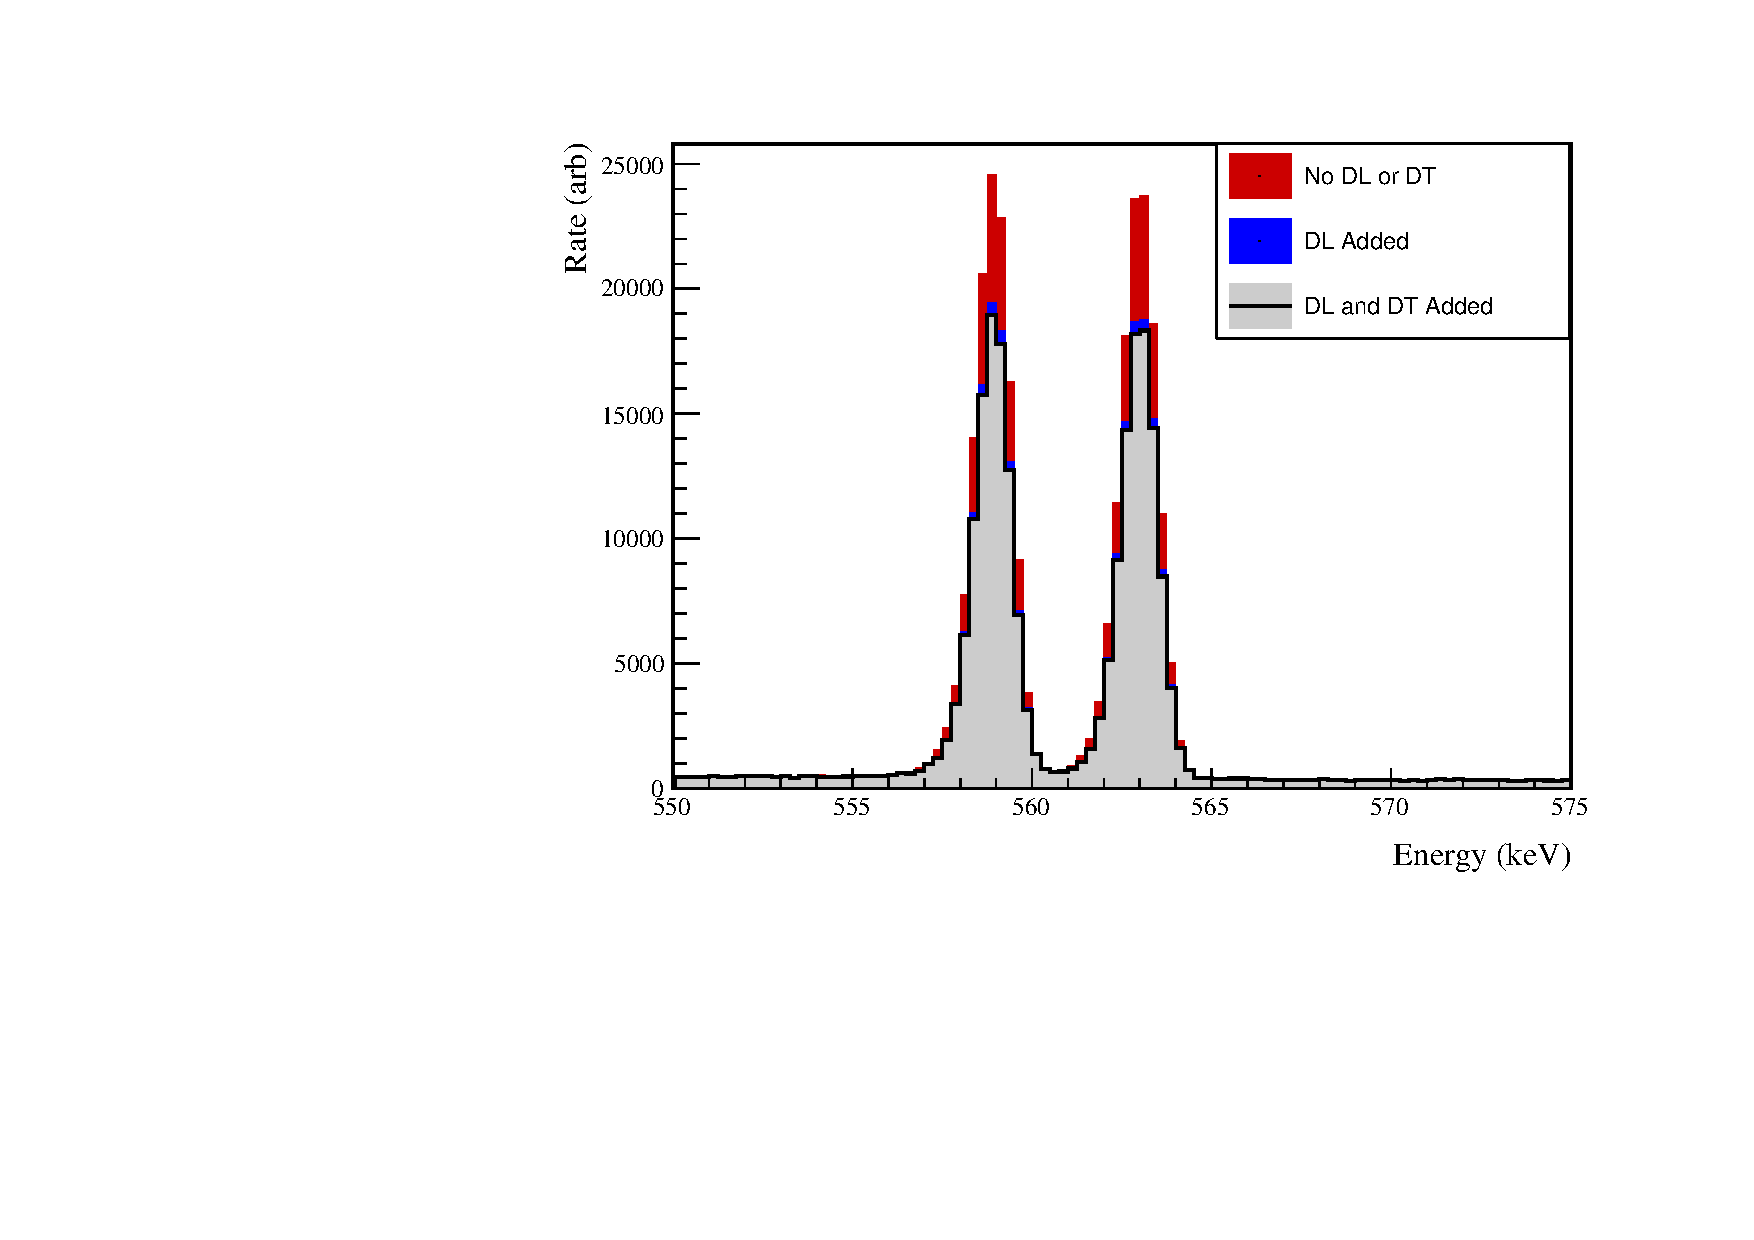
\includegraphics[width=0.8\textwidth]{DeadLayerDeadTime}
  \caption[Simulated effect of dead layers and dead times]{\label{fig:dldt}
    Effect of dead layers and dead times on peak amplitudes for \tnbb\ to the \SP{0}{+}{1} peaks in \msmd\ events.
  }
\end{figure}

\subsection{Dead Time Effects} \label{sec:DT}
Detector dead times, which affect only a single detector at a time, reduce the detection efficiency for events that occur in all detectors in the module.
For this reason, instead of subtracting these dead times from the livetime, the dead times are incorporated into the detection efficiency.
Detector dead times are measured individually for each run by counting pulser events and comparing to the number of expected pulser events for each detector.
The program \texttt{es\_livetime} collects the detector dead times that are measured in this way and finds the average detector dead time for each subdataset.
These dead times are then applied to the simulation skimming process as described in Section~\ref{sec:simskim}.
Similar to the dead layers, simulation files are produced with and without dead times in order to measure the size of the effect.
Uncertainties in the detector dead times are measured as the statistical uncertainties from pulser counts.
The percent uncertainty in efficiency loss from detector dead times is assumed to be the same as the average percent uncertainty in the detector dead time.
Typical loss of efficiency from detector dead times range from 1-3\%.
For the \tnbb\ to the \SP{0}{+}{1} decay, the losses are 2.5\% for module~1 and 1.9\% for module~2.
The effects of detector dead times can be seen in Figure~\ref{fig:dldt}.

\subsection{Simulation Validation and Errors} \label{sec:Co56}
In addition to dead layer and dead time effects that can be explicitly accounted for, other possible sources of systematic uncertainty from the simulation exist, such as inaccuracies in the simulation geometry.
To account for these, we use pair production events from calibration runs as a proxy for \bbes\ events.
In pair production events, an electron-positron pair is produced in the bulk of a detector, followed promptly by two 511~keV $\gamma$s from the annihilation of the positron.
Because these events involve a single pair production site and the prompt emission of gamma rays which may be absorbed in a separate detector, they make a good proxy for \bbes\ events.
In single-escape peak (SEP) events, one gamma is absorbed in the detector containing the pair-production, while the other escapes, resulting in a source detector hit with energy equal to the $\gamma$ energy minus 511~keV.
In double-escape peak (DEP) events, both gammas escape the detector, resulting in a source detector hit with energy equal to the $\gamma$ energy minus 1022~keV.
Both SEP and DEP events present the possibility for a second 511~keV detector hit.
By comparing the rate of multiplicity-1 events in the SEPs and DEPs to the rate of multiplicity-2 events in which one hit falls into one of these peaks and the other falls into the 511~keV peak, we can measure a proxy for the detection efficiency of our multi-site event signature.
By comparing this measurement to simulation, we can estimate the size of any unknown uncertainties in our simulation-based efficiency estimate.

\begin{figure}[t]
  \centering
  \subfloat{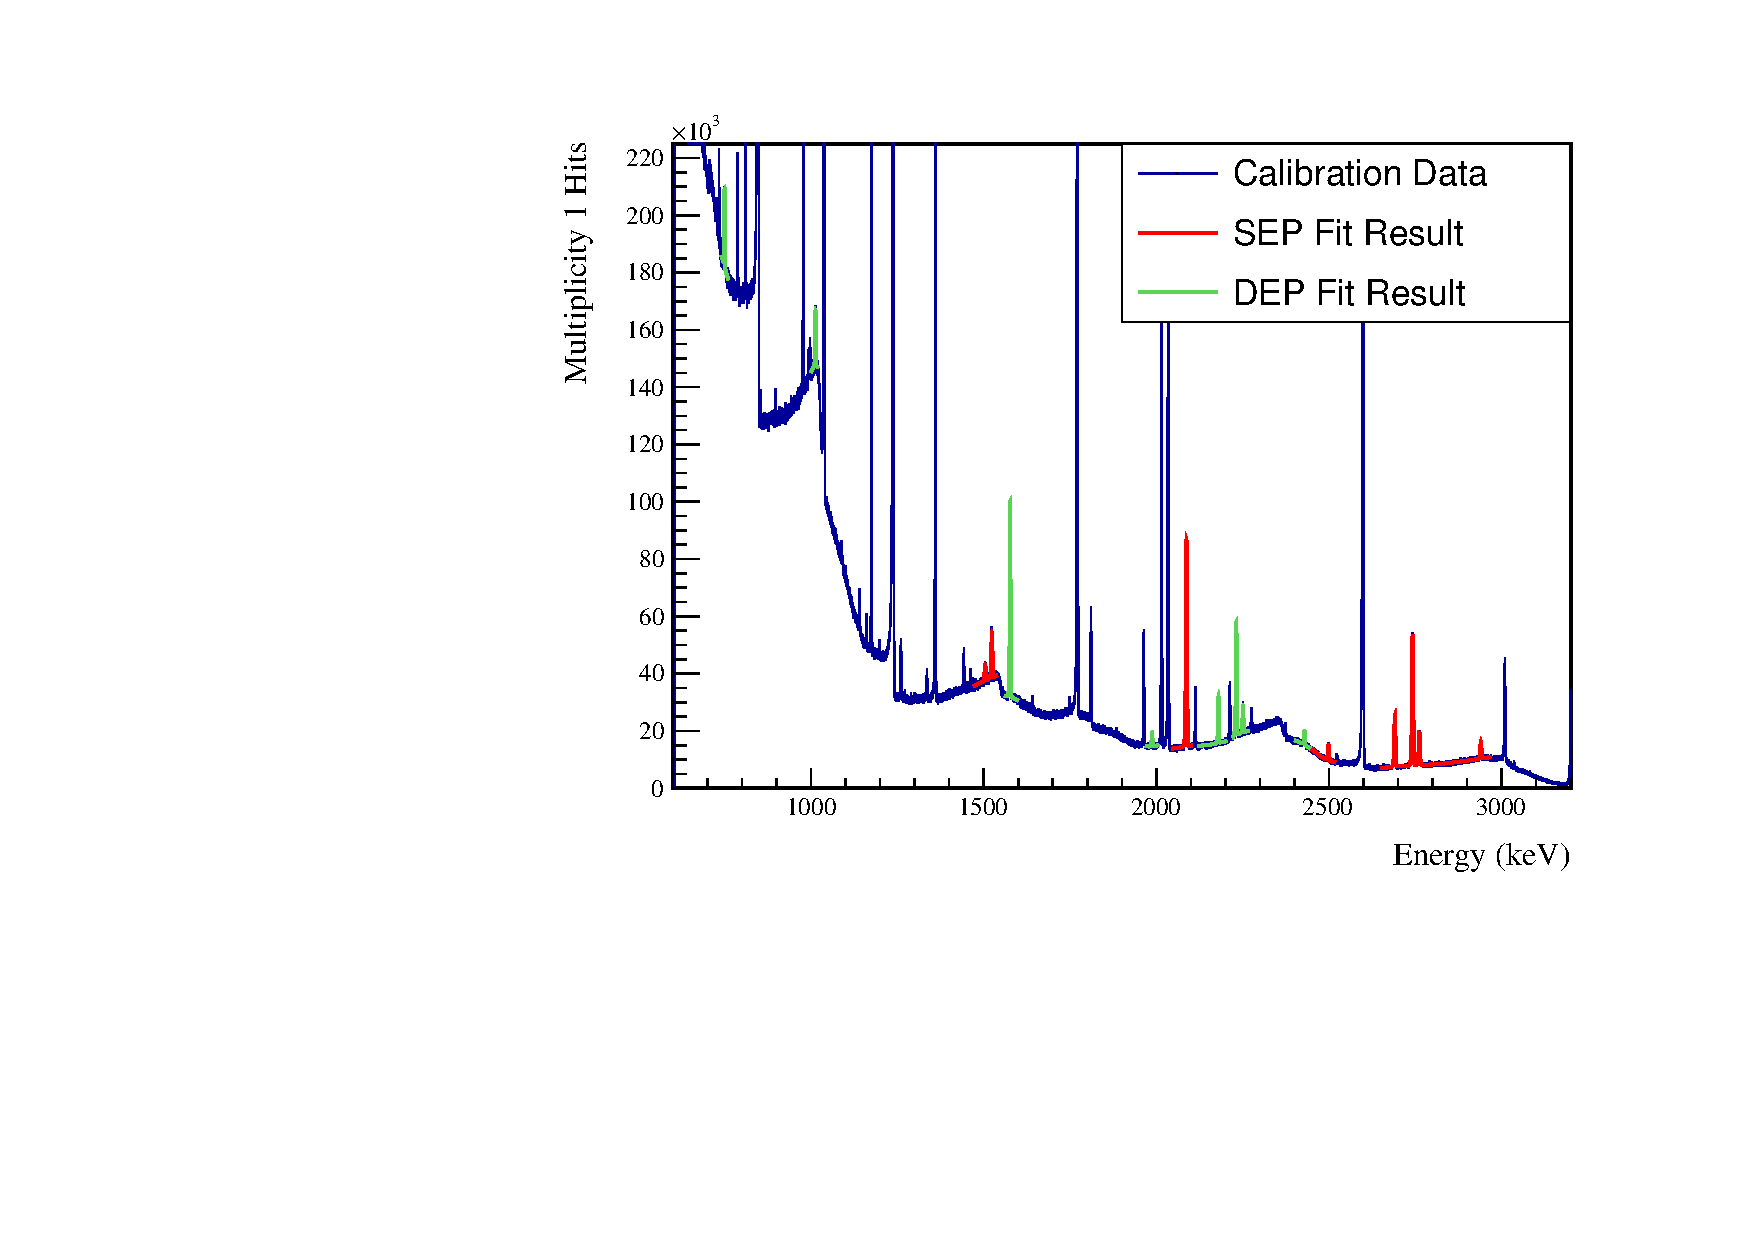
\includegraphics[width=.5\linewidth]{mult1Co56Fits}}
  \subfloat{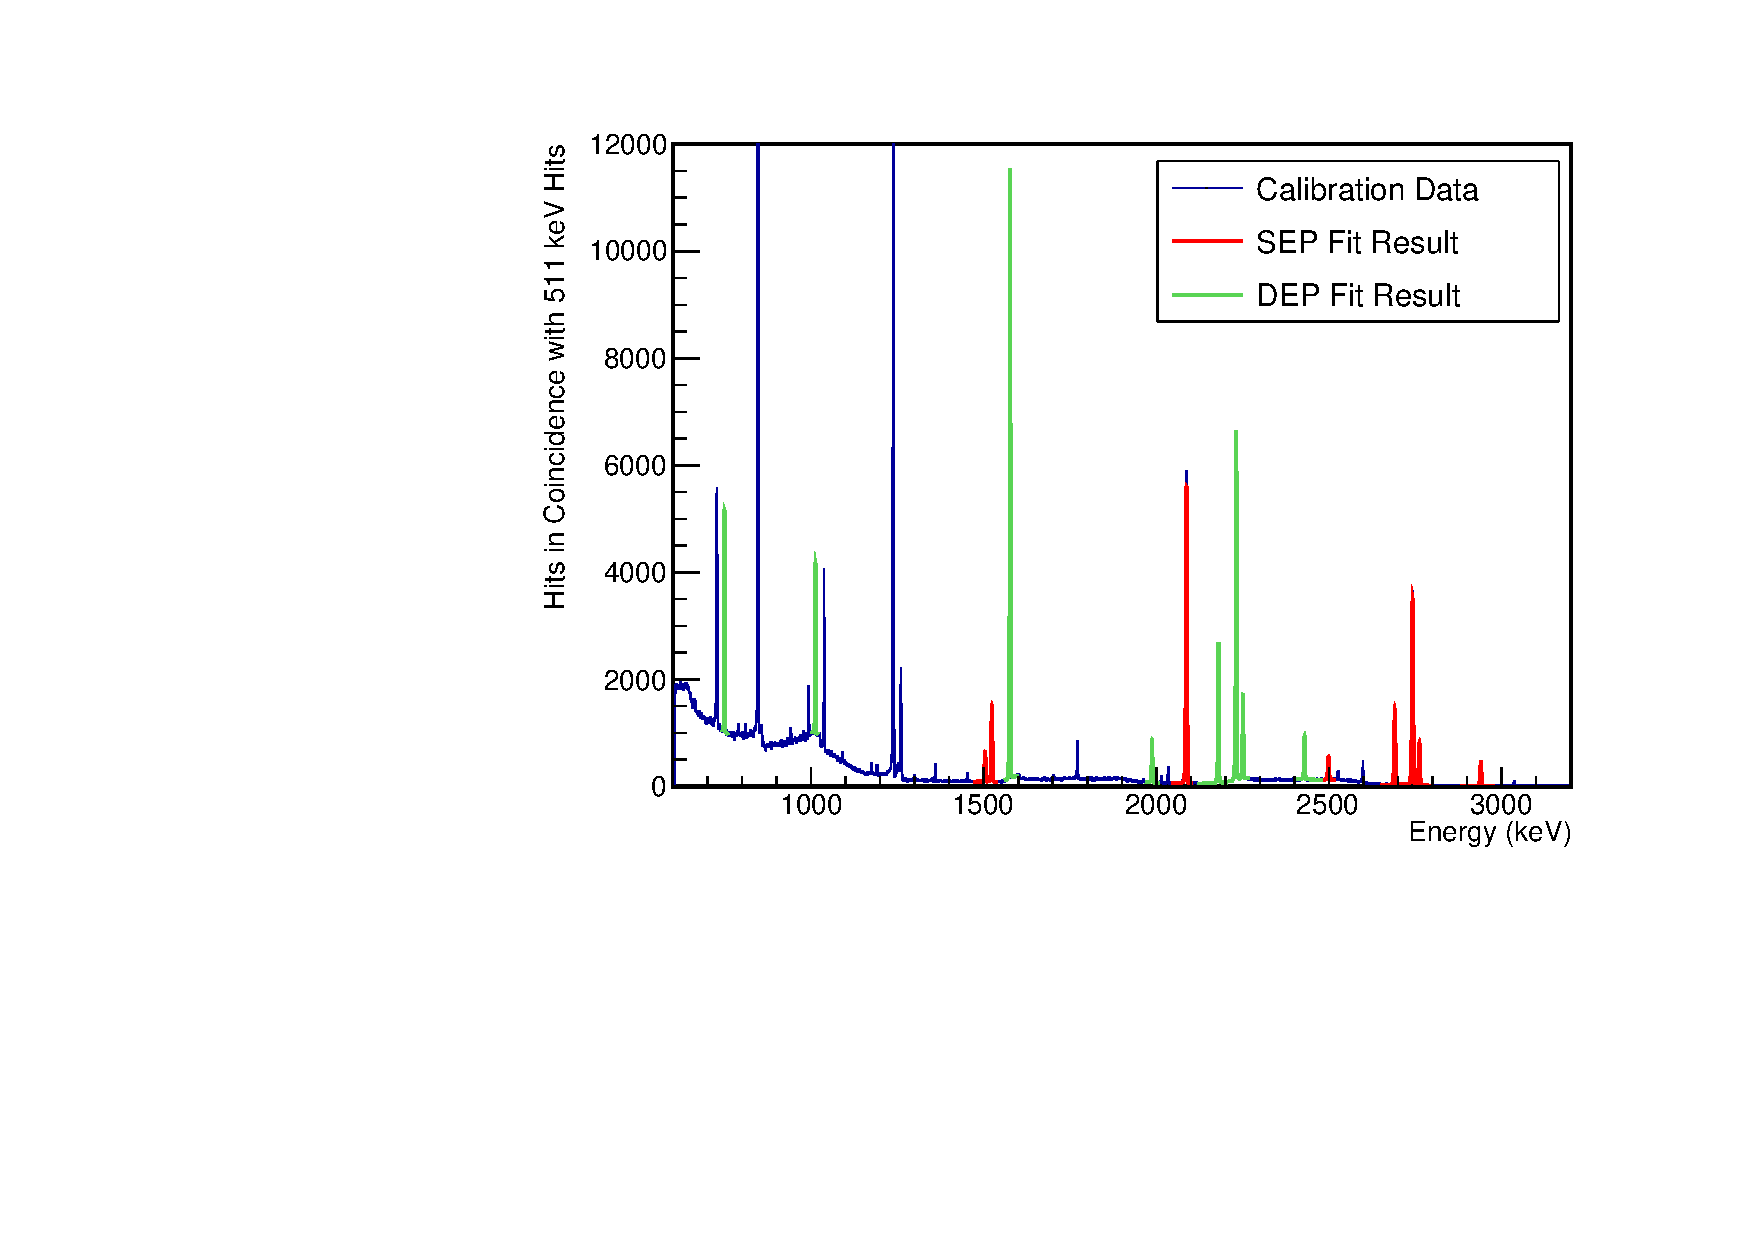
\includegraphics[width=.5\linewidth]{mult2Co56Fits}}
  \caption[Spectra of multiplicty 1 and 2 \Co{56} data with peak fits]{\label{fig:Co56Spectra}
    Spectra are shown of multiplicity 1 \Co{56} events (left) and multiplicity 2 \Co{56} events in coincidence with an annihilation gamma. The results of the simultaneous peak fits are drawn in red (SEP fit) and green (DEP fit).
  }
\end{figure}
To achieve this, we will use a \Co{56} calibration source.
\Co{56} presents the advantage of a large number of $\gamma$s at energies high enough to cause pair production, which allows for a comparison of many peaks to our simulation.
A \Co{56} line source was inserted into the module~1 calibration track on January 15, 2019 and 168.1~h of data were recorded, until January 22, 2019.
Immediately after this, the source was inserted into the module~2 calibration track and 167.1~h of data were recorded until January 29, 2019.
The source had a nominal activity of 6~kHz, resulting in a high enough data rate that the energy threshold for each channel was raised to ${\sim}400$~keV.
As discussed in Section~\ref{sec:calsims}, 3~billion event primaries were simulated for the \Co{56} source in each module's source track in order to achieve similar events statistics for both the simulations and data.
Simulations were run with and without dead layers.

8 SEPs and 7 DEPs were selected as proxies for the \bbes\ signal; these peaks were selected because of their prominence above the Compton continuum and the absense of nearby peaks that would interfere with a peak-height measurement.
A simultaneous fit, using the multipeak fitter, of all SEPs as single-detector events and as two-detector events in coincidence with a 511~keV peak event was performed in the calibration data and in the simulations both with and without dead layers.
SEPs and DEPs have abnormal peakshapes due to in-flight annihilation of the positrons, which results in Doppler broadening of the peaks.
For this reason, a high energy tail is added to the typical peak shape function.
The peak height ratios and uncertainties for peak $k$ are determined as follows:
\begin{equation}
  \epsilon_k=\frac{A_{k,m2}}{A_{k,m1}}
\end{equation}
\begin{equation}
  \sigma_{stat, k}=\epsilon_k \sqrt{\frac{\Sigma_{A,k,m1;A,k,m1}}{A_{k,m1}^2}-2\frac{\Sigma_{A,k,m1;A,k,m2}}{A_{k,m1}A_{k,m2}}+\frac{\Sigma_{A,k,m2;A,k,m2}}{A_{k,m2}^2}}
\end{equation}
where $A_{k,m1/2}$ are the fitted amplitudes of peak $k$ with multiplicity 1 and multiplicity 2 respectively, and $\Sigma_{A,k,m1/2;A,k,m1/2}$ is the fitted covariance matrix element for these amplitudes.
The same process of simultaneously fitting DEPs is followed to extract the DEP peak-height ratios.
The measured data spectra and fit results are shown in Figure~\ref{fig:Co56Spectra}.

\begin{figure}[t]
  \centering
  \subfloat{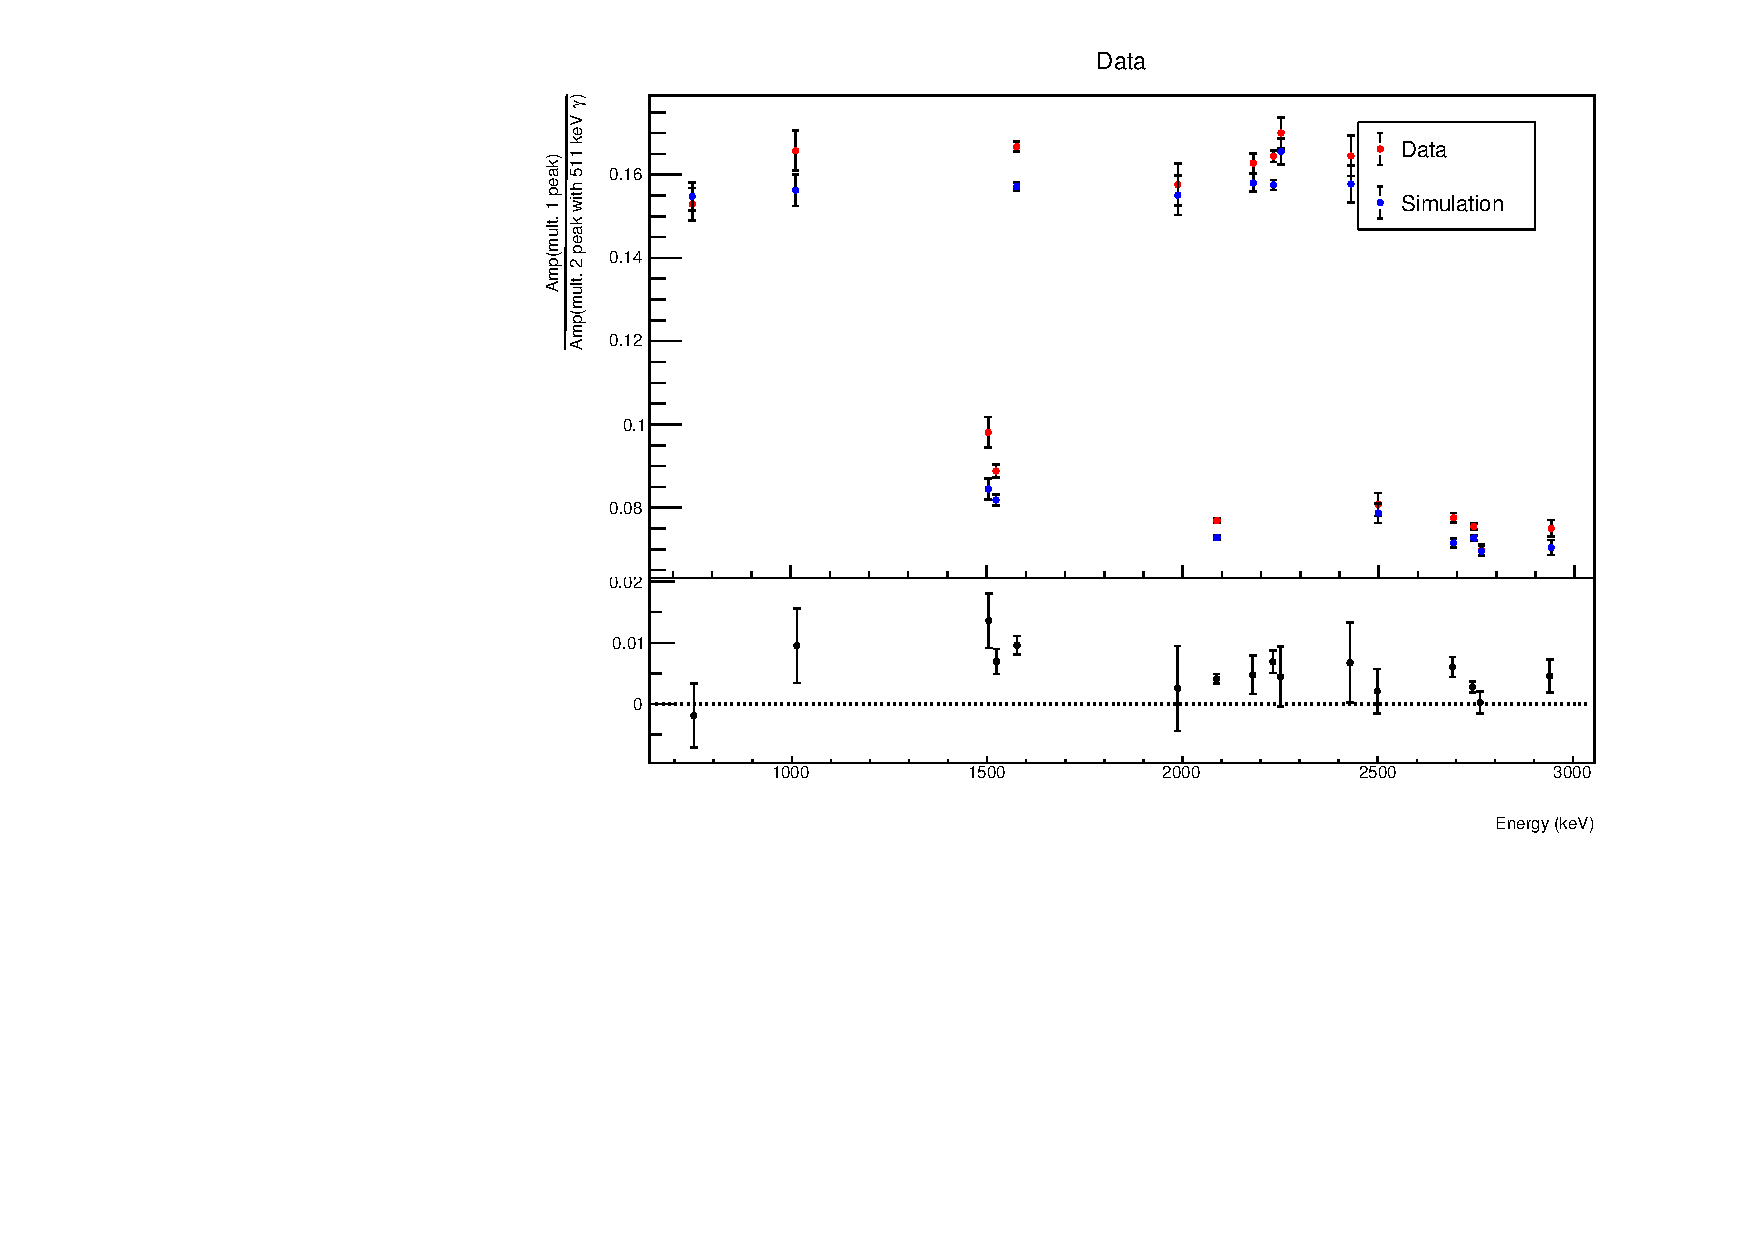
\includegraphics[width=.7\linewidth]{M1PeakRatioComparison}}
  \\
  \subfloat{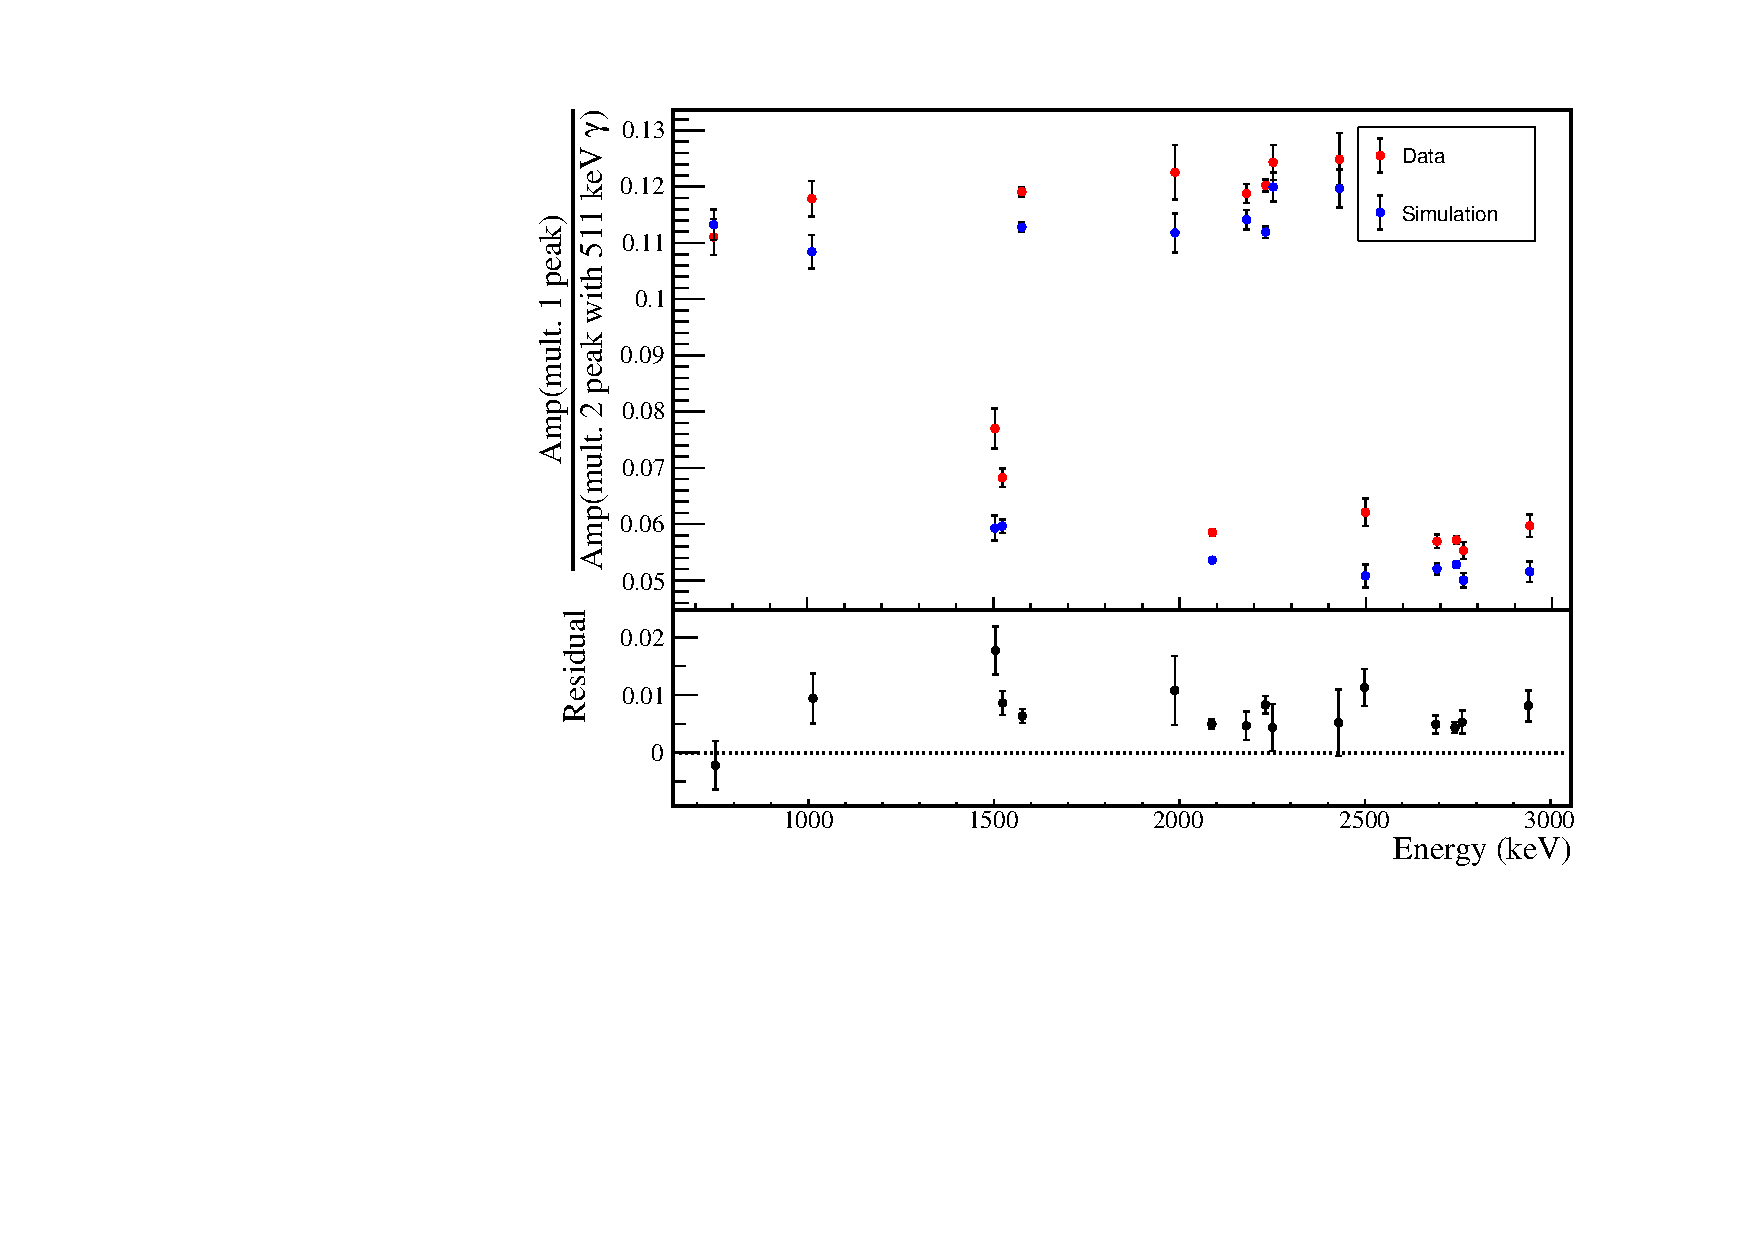
\includegraphics[width=.7\linewidth]{M2PeakRatioComparison}}
  \caption[Peak height ratio comparison results for module 1 and module 2]{\label{fig:co56results}
    Measurement of peak height ratios between multiplicity~1 events and multiplicity~2 events containing a 511~keV annihalation $\gamma$ for both simulated and measured \Co{56} spectra. Only statistical error bars are drawn. These ratios are listed in tables~\ref{tab:co56resultsM1} and \ref{tab:co56resultsM2}.
  }
\end{figure}
Figure \ref{fig:co56results} shows an overall offsete that cannot be explained by statistical errors; this discrepancy is measured and treated as a systematic error which will be applied to the \bbes\ measurement.
Since some of this discrepancy can be explained by the dead layer uncertainty, the difference between the simulated peak-height ratios with and without the dead layer is multiplied by the percent uncertainty in the dead layer thickness in order to measure the systematic error caused by the dead layer.
Finally, a $\chi^2$ value is computed for the comparison between the simulated and measured peak-heights using the statistical and dead layer uncertainties.
\begin{equation}
  \chi^2(\mu, \delta_{DL}) = \displaystyle\sum_{k=1}^N \frac{(\epsilon_{k, meas}-\epsilon_{k, sim}-\delta_{DL}\cdot\sigma_{DL,k} - \mu)^2}{\sigma_{stat,dat,k}^2+\sigma_{stat,sim,k}^2} + \delta_{DL}^2
\end{equation}
where $\sigma_{DL,k}$ is the uncertainty from dead layers, $\delta_{DL}$ is the measured error from dead layers (correlated across all peaks with a prior of 1~$\sigma$), and $\mu$ is the mean error that remains.
This $\chi^2$ function is minimized with respect to $\mu$ and $\delta_{DL}$ and the profile likelihood is used to compute the uncertainty on $\mu$, using MINUIT\cite{minuit}.
The systematic error is taken to be
\begin{equation}
  \sigma_{sim}^2 = \mu^2 + \sigma_\mu^2
\end{equation}
Tables~\ref{tab:co56resultsM1} and~\ref{tab:co56resultsM2} list the peak height ratios and uncertainties for each peak for module~1 and module~2, respectively.
The final fractional uncertainties measured are $\sigma_{sim,M1}=0.0020$ and $\sigma_{sim,M2}=0.0047$.
This uncertainty is applied directly to the detection efficiency measured before applying any other effects such as dead layers, dead times and cuts, without any scaling.
This uncertainty is one of the dominant uncertainties on the detection efficiency along with the dead layer uncertainty; while the absolute uncertainty is small, because it is applied to the detection efficiency, which tends to be ${\sim}5$\%, directly rather than to the loss from an individual effect, the fractional uncertainty is on the order of 10\%.
In cases where the detection efficiency is very low, such as the 1216~keV peak in module~2 from decays to the \SP{2}{+}{2} state, this uncertainty can completely overwhelm the detection efficiency.
Figure~\ref{fig:co56results} plots the peak height ratios for simulated and measured data for both modules~1 and~2.

\begin{table}[h]
  \caption[Table of peak height ratios for module~1]{\label{tab:co56resultsM1}
    Table of measured peak height ratios between multiplicity~1 events and multiplicity~2 events containing a 511~keV annihalation $\gamma$ in module~1 for both simulated and measured \Co{56} spectra, with uncertainties. A plot of these numbers is shown in Figure~\ref{fig:co56results}
  }
  \begin{tabular}{|c|c c c|c c c|c c|}
\hline
  Peak & $\frac{A_{m2,dat}}{A_{m1,dat}}$ & $\frac{A_{m2,sim}}{A_{m1,sim}}$ & $\frac{A_{m2,noDL}}{A_{m1,noDL}}$ & $\sigma_{dat,stat}$ & $\sigma_{sim,stat}$ & $\sigma_{sim,DL}$ & Residual & $\sigma_{resid}$ \\
\hline
  1504 keV (SEP) & 0.098 & 0.084 & 0.110 & 0.004 & 0.003 & 0.004 & 0.014 & 0.004 \\
  1524 keV (SEP) & 0.089 & 0.082 & 0.109 & 0.002 & 0.001 & 0.005 & 0.007 & 0.002 \\
  2088 keV (SEP) & 0.077 & 0.073 & 0.098 & 0.001 & 0.001 & 0.004 & 0.004 & 0.001 \\
  2499 keV (SEP) & 0.081 & 0.079 & 0.108 & 0.003 & 0.002 & 0.005 & 0.002 & 0.004 \\
  2691 keV (SEP) & 0.078 & 0.072 & 0.099 & 0.001 & 0.001 & 0.005 & 0.006 & 0.002 \\
  2743 keV (SEP) & 0.075 & 0.073 & 0.101 & 0.001 & 0.001 & 0.005 & 0.003 & 0.001 \\
  2762 keV (SEP) & 0.070 & 0.070 & 0.096 & 0.001 & 0.001 & 0.004 & 0.000 & 0.002 \\
  2940 keV (SEP) & 0.075 & 0.070 & 0.100 & 0.002 & 0.002 & 0.005 & 0.005 & 0.003 \\
  749 keV (DEP) & 0.153 & 0.155 & 0.225 & 0.004 & 0.003 & 0.012 & -0.002 & 0.005 \\
  1013 keV (DEP) & 0.166 & 0.156 & 0.229 & 0.005 & 0.004 & 0.012 & 0.010 & 0.006 \\
  1577 keV (DEP) & 0.167 & 0.157 & 0.224 & 0.001 & 0.001 & 0.011 & 0.010 & 0.002 \\
  1988 keV (DEP) & 0.158 & 0.155 & 0.222 & 0.005 & 0.005 & 0.011 & 0.003 & 0.007 \\
  2180 keV (DEP) & 0.163 & 0.158 & 0.225 & 0.002 & 0.002 & 0.011 & 0.005 & 0.003 \\
  2232 keV (DEP) & 0.164 & 0.158 & 0.225 & 0.001 & 0.001 & 0.012 & 0.007 & 0.002 \\
  2251 keV (DEP) & 0.170 & 0.166 & 0.233 & 0.004 & 0.003 & 0.011 & 0.004 & 0.005 \\
  2429 keV (DEP) & 0.165 & 0.158 & 0.230 & 0.005 & 0.004 & 0.012 & 0.007 & 0.007 \\
\hline
\end{tabular}

\end{table}

\begin{table}[h]
  \caption[Table of peak height ratios for module~2]{\label{tab:co56resultsM2}
    Table of measured peak height ratios between multiplicity~1 events and multiplicity~2 events containing a 511~keV annihalation $\gamma$ in module~2 for both simulated and measured \Co{56} spectra, with uncertainties. A plot of these numbers is shown in Figure~\ref{fig:co56results}
  }
  \begin{tabular}{|c|c c c|c c c|c c|}
\hline
  Peak & $\frac{A_{m2,dat}}{A_{m1,dat}}$ & $\frac{A_{m2,sim}}{A_{m1,sim}}$ & $\frac{A_{m2,noDL}}{A_{m1,noDL}}$ & $\sigma_{dat,stat}$ & $\sigma_{sim,stat}$ & $\sigma_{sim,DL}$ & Residual & $\sigma_{resid}$ \\
\hline
  1504 keV (SEP) & 0.077 & 0.059 & 0.082 & 0.004 & 0.002 & 0.004 & 0.018 & 0.004 \\
  1524 keV (SEP) & 0.068 & 0.060 & 0.081 & 0.002 & 0.001 & 0.004 & 0.009 & 0.002 \\
  2088 keV (SEP) & 0.059 & 0.054 & 0.074 & 0.001 & 0.000 & 0.003 & 0.005 & 0.001 \\
  2499 keV (SEP) & 0.062 & 0.051 & 0.073 & 0.002 & 0.002 & 0.004 & 0.011 & 0.003 \\
  2691 keV (SEP) & 0.057 & 0.052 & 0.074 & 0.001 & 0.001 & 0.004 & 0.005 & 0.002 \\
  2743 keV (SEP) & 0.057 & 0.053 & 0.075 & 0.001 & 0.001 & 0.004 & 0.004 & 0.001 \\
  2762 keV (SEP) & 0.055 & 0.050 & 0.071 & 0.002 & 0.001 & 0.004 & 0.005 & 0.002 \\
  2940 keV (SEP) & 0.060 & 0.052 & 0.072 & 0.002 & 0.002 & 0.003 & 0.008 & 0.003 \\
  749 keV (DEP) & 0.111 & 0.113 & 0.155 & 0.003 & 0.003 & 0.007 & -0.002 & 0.004 \\
  1013 keV (DEP) & 0.118 & 0.108 & 0.156 & 0.003 & 0.003 & 0.008 & 0.009 & 0.004 \\
  1577 keV (DEP) & 0.119 & 0.113 & 0.161 & 0.001 & 0.001 & 0.008 & 0.006 & 0.001 \\
  1988 keV (DEP) & 0.123 & 0.112 & 0.153 & 0.005 & 0.003 & 0.007 & 0.011 & 0.006 \\
  2180 keV (DEP) & 0.119 & 0.114 & 0.164 & 0.002 & 0.002 & 0.008 & 0.005 & 0.002 \\
  2232 keV (DEP) & 0.120 & 0.112 & 0.160 & 0.001 & 0.001 & 0.008 & 0.008 & 0.001 \\
  2251 keV (DEP) & 0.124 & 0.120 & 0.170 & 0.003 & 0.003 & 0.008 & 0.004 & 0.004 \\
  2429 keV (DEP) & 0.125 & 0.120 & 0.159 & 0.005 & 0.003 & 0.007 & 0.005 & 0.006 \\
\hline
\end{tabular}

\end{table}

\section{Region of Interest Selection}
Once the multi-site events have been collected, we want to search for detector hits with the energies of the $\gamma$s emitted in each \bbes\ decay mode.
To do this, a signal region of interest (ROI) must be identified.
To estimate the number of background events in the signal ROI, a background ROI must also be selected near the signal ROI.
This section will describe the selection of the signal and background ROIs and the calculation of the efficiency and uncertainties on the efficiency due to the ROI selection.

For each dataset, a simultaneous fit of many peaks is performed to a combined spectrum of all detectors and all calibration runs, ensuring that any variation in gain or energy nonlinearity between detectors is accounted for.
From each fit result, a set of parameters describing a single peak at the energy of the signal ROI can be extracted, along with a covariance matrix for those parameters.
From these fit results, we can compute the optimal ROI, detection efficiency and uncertainty for each data set.
An example of a calibration spectrum with the FWHM curve fit to it is shown in Figure~\ref{fig:fwhmcal}.
\begin{figure}[h]
  \centering
  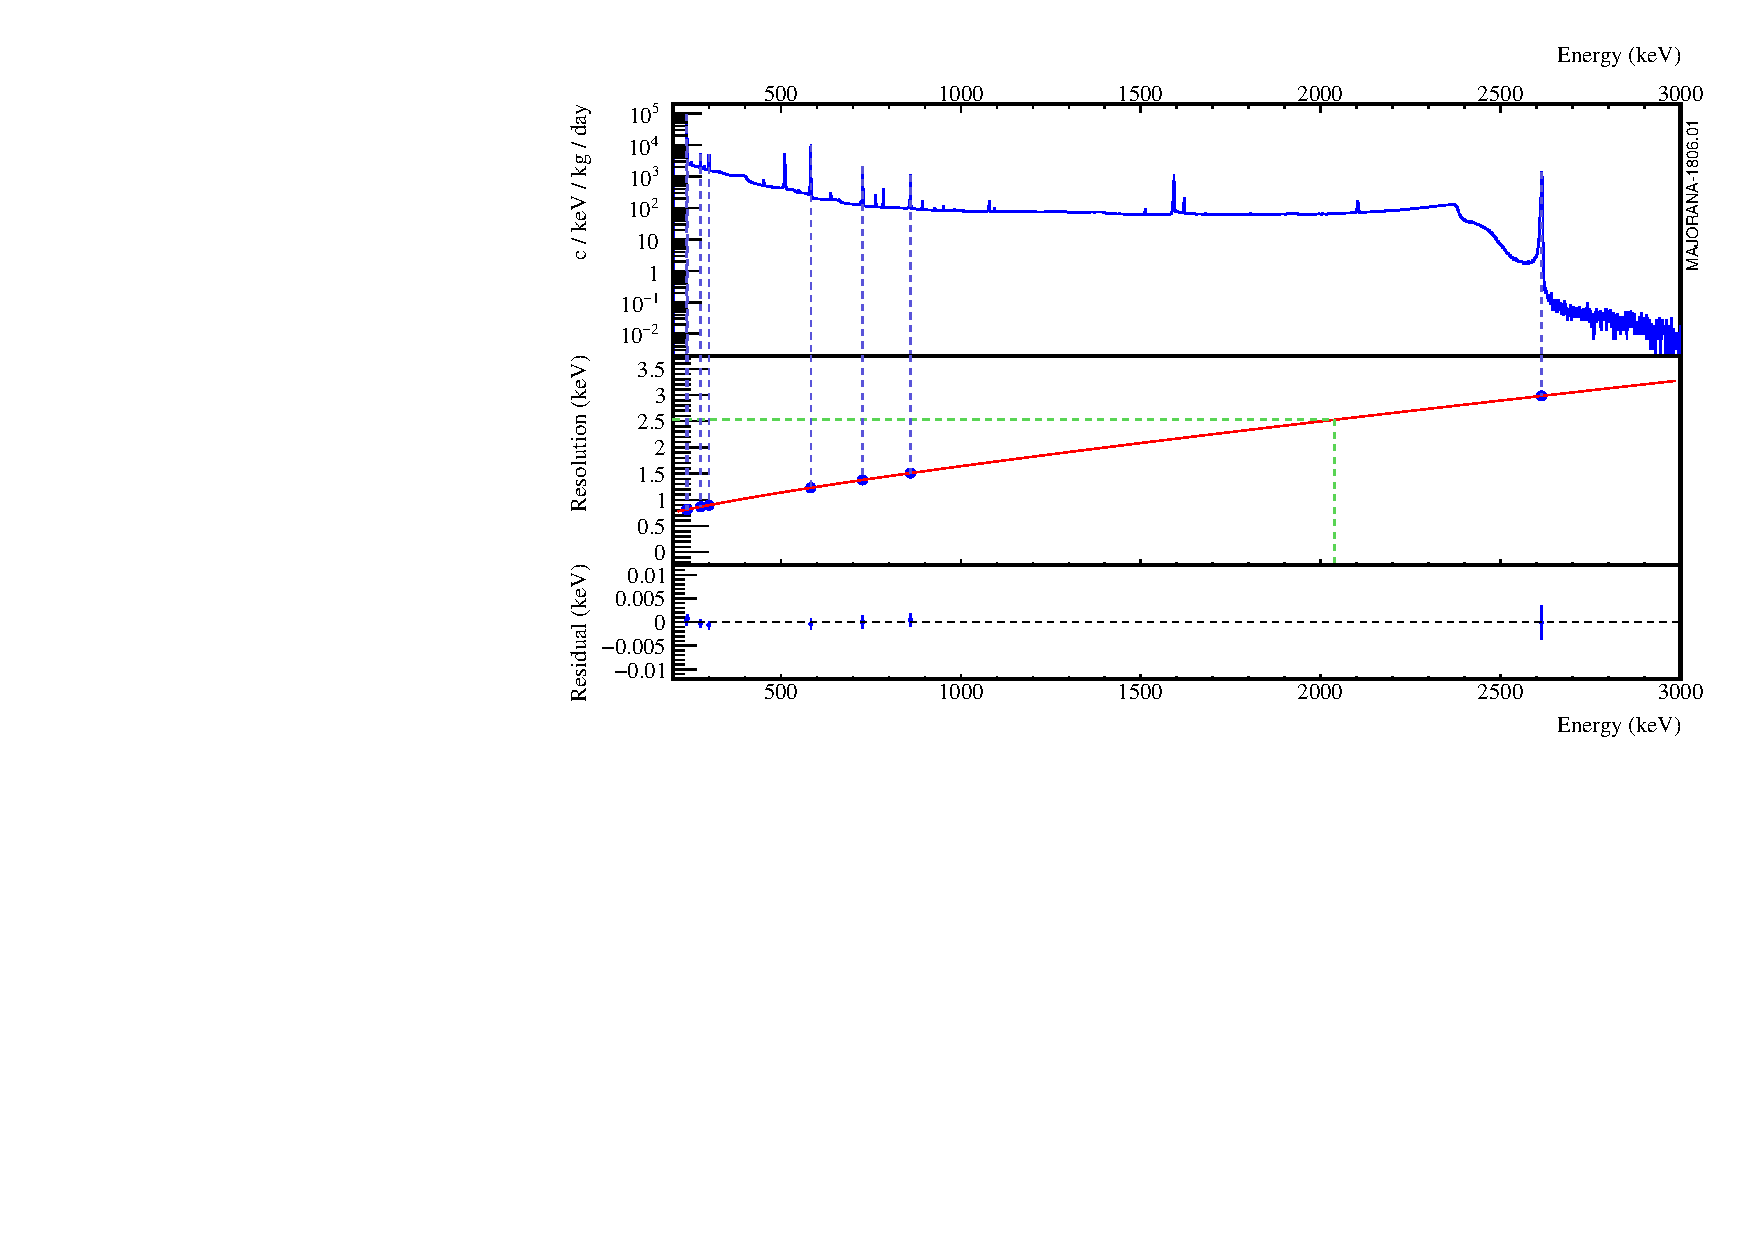
\includegraphics[width=.9\linewidth]{fwhmcal}
  \caption[FWHM extracted from a \Th{228} calibration spectrum]{\label{fig:fwhmcal}
    A \Th{228} calibration run with the FWHM fit curve and individual uncertainties at several peaks. This curve is used to compute the FWHM for a peak at a given energy. The statistical uncertainties are extracted from the fit result. An additional systematic uncertainty is added to account for the residuals.
  }
\end{figure}

\subsection{Signal ROI Optimization} \label{sec:roiopt}
The signal region of interest around each peak is optimized based on the peak shape functions as fit for each data set.
The optimization follows the procedure laid out in Appendix~\ref{app:sens} and maximizes the rate sensitivity with respect to the region of interest upper and lower boundaries, $E_{low}$ and $E_{high}$ respectively:
\begin{equation}
  \hat\Gamma(E_{low}, E_{high}, \overline B) \propto \frac{\mathrm{DP}\big(\overline B(E_{high}-E_{low})\big)}{\epsilon_{ROI}(E_{low}, E_{high})}
\end{equation}
where $\mathrm{DP}$ is the discovery potential as defined in Appendix~\ref{app:sens}, and a flat background with background index $\overline B$ measured from data is assumed.
The efficiency is defined by the CDF of the Gaussian and LE tail components
\begin{equation}
  \label{eq:PSCDF}
  \begin{aligned}
    \epsilon_{ROI}(E_{low}, E_{high}; \mu, \sigma, f_{tail}, \tau) &= \frac{1}{2}\big(\mathrm{erfc}\left(\frac{E_{low}-\mu}{\sqrt{2}\sigma}\right) - \mathrm{erfc}\left(\frac{E_{high}-\mu}{\sqrt{2}\sigma}\right)\big) \\& + f_{tail}\tau\big(\mathrm{ExGaus}(E_{high}; \mu, \sigma, \tau)-\mathrm{ExGaus}(E_{low}; \mu, \sigma, \tau)\big)
  \end{aligned}
\end{equation}
The optimal ROI is numerically calculated by minimizing $\frac{1}{\hat\Gamma(E_{low}, E_{high}, \overline B)}$ with respect to $E_{low}$ and $E_{high}$ using MINUIT\cite{minuit}.

\subsection{Background ROI Selection}
For each peak, a background ROI of width $50-100$~keV surrounding the peak is selected.
The ROI is selected to avoid any known background peaks and exclude them with at least $99.9\%$ efficiency.
A $99.9\%$ exclusion region calculated from the peakshape function is selected around the peak and removed from the background ROI.

\subsection{ROI Detection Efficiency and Uncertainty} \label{sec:ROIEff}
The ROI detection efficiency is calculated from the CDF defined in Equation~\ref{eq:PSCDF}.
The covariance matrix of the peak shape parameters obtained from the fit result is used to calculate the statistical uncertainty of the efficiency.
Several additional systematic effects must also be accounted for:
\begin{itemize}
\item \textbf{Gain drift:} \Th{228} energy calibrations are taken once per week, for 90 minutes each.
  In between these calibration runs, the energy calibration parameters undergo small adjustments that result in energy inaccuracies for background runs taken in between.
  This gain drift results in an increase in the width of the peak, which is accounted for by adding in quadrature $\sigma_{drift}$ to the value of $\sigma$ obtained from the fit.
  This also results in the dominant systematic uncertainty on the peak width, $\delta_{fwhm,drift}$.
  The gain drift also results in a small systematic error in the measured energy of the peak $\delta_{\mu,drift}$.
  A detailed description of the measurement of this systematic effect is contained in Reference~\cite{energysystunidoc}.  
\item \textbf{Energy nonlinearity:} While the energy response for HPGe detectors is ostensibly linear, several factors result in small nonlinearities.
  Local nonlinearities that are correlated over small energy scales of arise from the response of the Gretina digitizers.
  While these nonlinearities are corrected for, a residual nonlinearity of ${\sim}0.1$~keV with a period of ${\sim}300$~keV remains.
  Global nonlinearities result from systematic uncertainties in the energy estimation.
  One source of global nonlinearity arises from uncertainty in the start time of the waveform, which is energy dependant.
  Another is a small quadratic term resulting from charge recombination.
  Because calibrations are performed on peaks with energies ranging from 238~keV to 2614~keV, energy shifts due to global nonlinearities are very small in this range and local energy nonlinearities dominate.
  At smaller and larger energies, the shifts can be as large as ${\sim}0.5$~keV in some detectors.
  In addition to this bias, energy nonlinearities result in an increase in $\sigma$ as a result of the combining of peaks from different detectors with different shifts; however, since the energy calibrations include all detectors, this shift is already included in the fit result, so no action is required.
  Energy nonlinearities also have a significant affect on the uncertainty in the measured peak energy, $\delta_{\mu,NL}$, which is a dominant uncertainty.
  A detailed description of the measurement of each of these systematic effects is contained in Reference~\cite{energysystunidoc}.
\item \textbf{Detector Crosstalk:} Because we are searching for peaks in coincidence events, the possibility for a distortion in the energy measurement due to crosstalk between the involved events exists.
  This effect is measured in Section~\ref{sec:crosstalk} to be small enough that no energy correction or peakshape correction is required.
  However, this effect does contribute to small uncertainties in the peak position, $\delta_{\mu,xtalk}$ and peak width, $\delta_{fwhm,xtalk}$.
\end{itemize}

Once these uncertainties have been measured, they must be propagated into the detection efficiency.
The statistical and systematic uncertainties on $\mu$ and the FWHM are added in quadrature to obtain $\delta_\mu$ and $\delta_{fwhm}$.
The uncertainty on the FWHM is used to calculate a width scale uncertainty, $\delta_\alpha$, which is simply the fractional uncertainty on the FWHM.
To compute the uncertainty on the efficiency, the efficiency is computed after modifying the peakshape parameters by one-sigma in either direction.
For the uncertainty from the width, we take:
\begin{equation}
  \begin{aligned}
    \sigma_{\epsilon_{ROI},fwhm} = \frac{1}{2}&\big(\epsilon_{ROI}(E_{low}, E_{high}; \mu, \sigma(1+\delta_\alpha), f_{LE}, \tau(1+\delta_\alpha)) \\&- \epsilon_{ROI}(E_{low}, E_{high}; \mu, \sigma(1-\delta_\alpha), f_{LE}, \tau(1-\delta_\alpha))\big)
  \end{aligned}
\end{equation}
Because the ROI is optimized around $\mu$, shifts in the peak in either direction will cause a reduction in efficiency.
For this reason, we must perform a second order propagation of uncertainties with respect to $\delta_\mu$.
The result is a slight degradation in the efficiency, so that
\begin{equation}
  \epsilon_{ROI} =  \frac{\epsilon_{ROI}(E_{low}, E_{high}; \mu + \delta_\mu, \sigma, f_{LE}, \tau) + \epsilon_{ROI}(E_{low}, E_{high}; \mu - \delta_\mu, \sigma, f_{LE}, \tau)}{2}
\end{equation}
and
\begin{equation}
  \sigma_{\epsilon_{ROI},\mu} = \epsilon_{ROI}(E_{low}, E_{high}; \mu, \sigma, f_{LE}, \tau)) - \epsilon_{ROI}
\end{equation}
These uncertainties are taken to be uncorrelated and added in quadrature to obtain the final uncertainty on the ROI efficiency.
Table~\ref{tab:energysystematics} contains a full summary of all of the energy uncertainties, the ROIs, and the ROI efficiencies and uncertainties.
\begin{sidewaystable}[p]
  \caption[Energy systematics]{ \label{tab:energysystematics}
    Table of energy estimation uncertainties, regions of interest, and efficiencies
  }
  \resizebox{\textwidth}{!}{%
  ../../appAllResults/tables/table_2vBB_ES0_1_pseff.tex }
\end{sidewaystable}

\subsection{Detector Crosstalk} \label{sec:crosstalk}
Detector crosstalk is caused when a true signal in one detector channel induces a small signal in another channel.
This is not a large enough effect to trigger events in a separate channel, meaning that it does not effect single-detector events.
However, it could produce an energy estimation error in multi-detector events since coincident pulses could induce signals that interfere either constructively or destructively, shifting the measured energies.
In practice, this could produce both a shift and additional uncertainty in both the measured energy of the peak and in the width of the peak.
To check for this effect, we can look at multi-detector events in \Th{228} calibration data.
In particular, we will compare the centroid and FWHM for several peaks in both single-detector events and multi-detector events.
\begin{figure}[h]
  \centering
  \subfloat{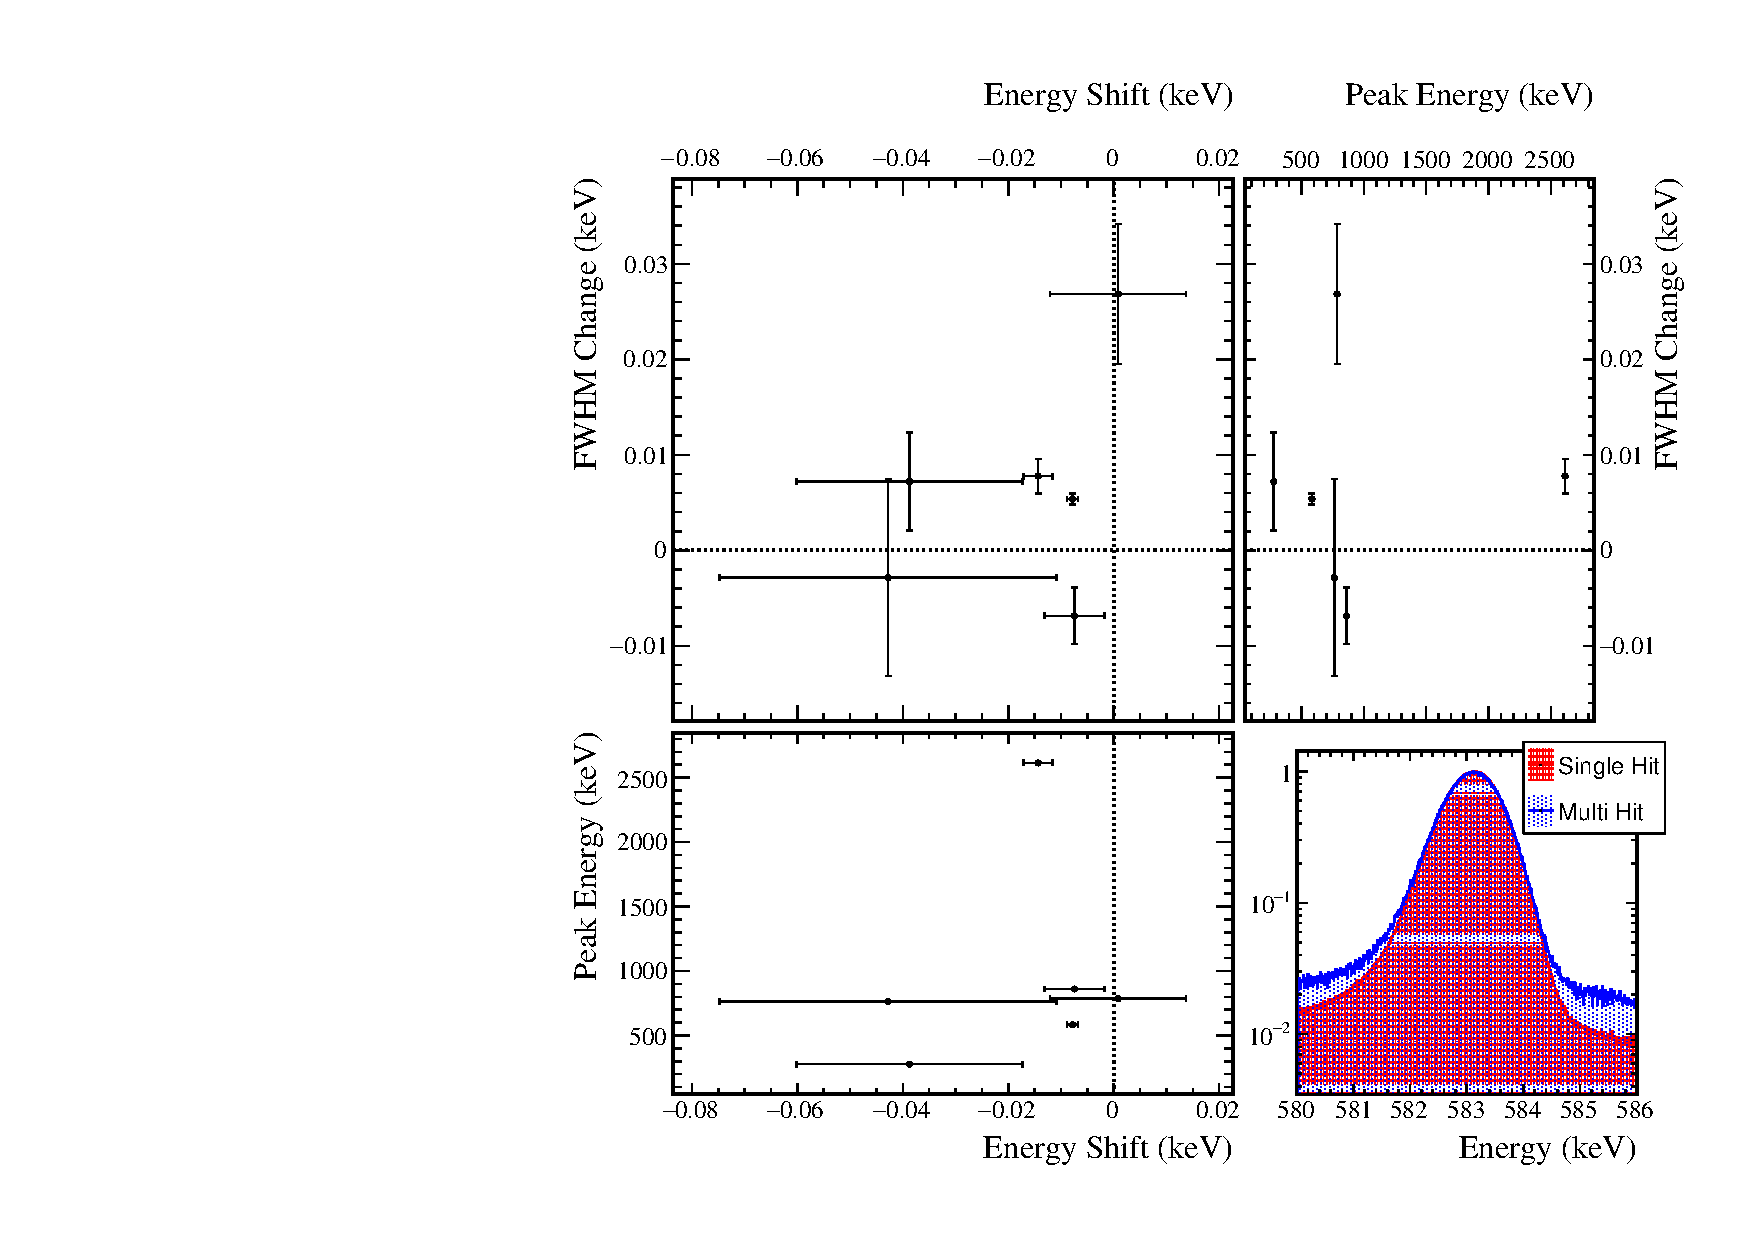
\includegraphics[width=\linewidth]{xtalkplot}}
  \caption[Peak shape comparison for single- and multi-detector events]{\label{fig:xtalk}
    Difference of the measured centroid and FWHM of several \Th{228} calibration peaks. Error bars represent the fit errors. Notice on the bottom right, that any difference is not visible to the naked eye.
  }
\end{figure}

5 peaks were selected from the \Tl{208} $\gamma$ cascade, at 277, 583, 763, 860 and 2614~keV, and one additional peak was selected from the \Bi{212} cascade, at 785~keV.
These peaks were selected based on their prominence in the high multiplicity hit spectrum.
The combined calibration spectra from dataset~6 were used to perform this analysis.
These peaks were fit individually, and the centroid and FWHM were computed for multiplicity 1~and multiplicity~2 events.
Figure~\ref{fig:xtalk} shows the results of these measurements.
While a very small reduction in peak centroid and increase in peak width are observed, the shifts are small compared to the existing uncertainties in these parameters.
As a result, we will ignore this shift and instead compute an uncertainty in each parameter caused by crosstalk.
We will treat the systematic error as uncorrelated between the peaks and compute the necessary error needed to make the combined statistical and systematic errors large enough to make the $\chi^2$ value computed by comparing these peaks equal to 1:
\begin{equation}
  \chi^2 = \displaystyle\sum_{k=0}^N \frac{(\mathrm{cen}_{k,m1} - \mathrm{cen}_{k,m2})^2}{\sigma_{cen,k,m1}^2+\sigma_{cen,k,m2}^2+\delta_{\mu,xtalk}^2}
\end{equation}
\begin{equation}
  \chi^2 = \displaystyle\sum_{k=0}^N \frac{(\mathrm{FWHM}_{k,m1} - \mathrm{FWHM}_{k,m2})^2}{\sigma_{fwhm,k,m1}^2+\sigma_{fwhm,k,m2}^2+\delta_{fwhm,xtalk}^2}
\end{equation}
Both systematic errors are numerically computed using a Brent minimization algorithm\cite{brent}.
The results are $\delta_{\mu,xtalk}=0.012$~keV and $\delta_{fwhm,xtalk}=0.011$~keV, both of which are subdominant uncertainties.


\section{Background Cuts}
By making use of known properties of background events, data cleaning cuts can be designed to selectively reduce backgrounds while minimizing sacrifice of excited state events.
Because of the \md\ nature of the event selection, many of these background cuts are designed to make use of observables from the detector hits in coincidence with candidate hits.

\subsection{Enriched Source Detector Cut}
Since the \bbes\ events must originate in \Ge{76}, events are far likelier to originate in enriched HPGe detectors than those with natural germanium isotopic abundances.
There are 29.8~kg of enriched detectors, with $88.1 \pm 0.7$\% abundance of \Ge{76} and 14.4~kg of natural detectors, with $7.83 \pm 0.07$\% abundance of \Ge{76}.
This means that $95.8 \pm 0.1$\% of \bbes\ events will originate in enriched detectors.
If we assume that background events will hit all detector mass at the same rate, then we would expect only 67\% of hits from background events involving two detectors to be in coincidence with a hit in an enriched detector.
This means that a significant gain in sensitivity can be acheived by cutting hits that are not in coincidence with an enriched detector hit.
While the detection efficiency of this cut is expected to be close to 95.8\%, the actual efficiency is measured from simulations, and tends to be greater, since a greater proportion of enriched detectors are active compared to natural detectors.

\begin{figure}[h]
  \centering
  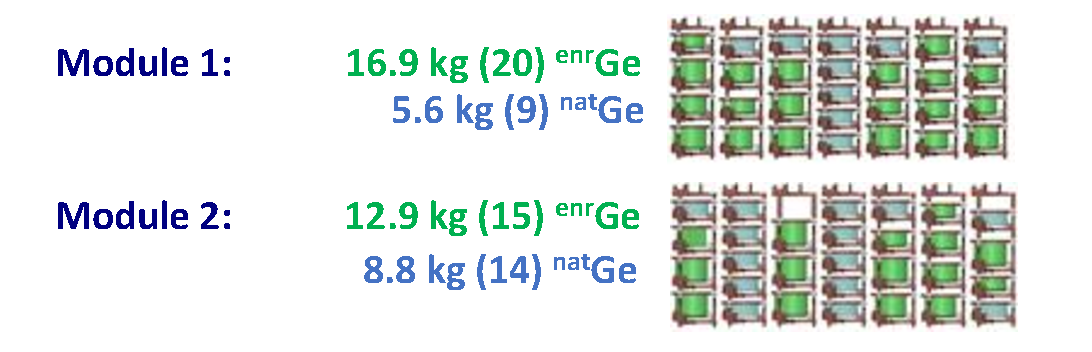
\includegraphics[width=0.8\textwidth]{enrnatdets}
  \caption[Module 1 and Module 2 enriched and natural detectors]{\label{fig:Ge76BBLevelDiagram}
    Diagram showing each detector in each module, arranged by which string and position they are in. Enriched detectors are colored green and natural detectors are colored blue. 95\% of \Ge{76} in the array is contained in the enriched detectors.}
\end{figure}

\subsection{Coincident and Sum Energy Cuts} \label{sec:MSenergycuts}
The greatest source of background events is expected to be $\gamma$-rays from a handful of known primordial and cosmogenic isotopes.
Because $\gamma$-rays are monoenergetic, they will often present a clear detection signature that can be targeted.
$\gamma$-rays will often Compton scatter from one detector into another, depositing their entire energy between the two.
For this reason, events whose total energy is equal to the energy of a known $\gamma$ can be cut.
$\beta$-decays will often result in a cascade of multiple $\gamma$s, at least one of which may be fully absorbed in a single detector.
These events can be cut by searching for a coincident detector with energy equal to that of a known $\gamma$.
Finally, whereas the \bb\ decay spectrum approaches zero amplitude at low energies and at \Qbb, the Compton continuum of $\gamma$s has a large amplitude at low energies.
This means that sensitivity can be gained by setting low- and high-energy thresholds on hits in coincidence with a candidate event.
These combined backgrounds can be reduced by cutting events with either sum energies or coincident hit energies that fall in a set of energy ranges.
For \bbes\ modes with multiple $\gamma$s, the optimal energy ranges will differ between natural and enriched detectors, since natural detectors will mostly include hits from one of the $\gamma$s, while enriched events will include \bb\ hits, $\gamma$ hits, and pileup events including both of these, allowing a much wider energy range.
For this reason, a separate set of coincident cut energy ranges are used for natural and enriched detectors.

The energy ranges that are cut can be determined by comparing the background model simulation to simulations of each \bbes\ decay mode.
An algorithm was written that simultaneously selects a set of both sum and coincident energy ranges to cut that optimizes discovery potential, as defined in Appendix~\ref{app:sens}.
The algorithm begins by identifying events in the \bbes\ simulation that include at least one hit consisting of the full absorption of a $\gamma$ photon and events in the background model simulation that include at least one hit in the background region of interest.
These events are then sorted into energy bins for each coincident hit and for the sum energy of the event (a single event will be in multiple bins).
For each bin, the algorithm checks the change in discovery potential if the bin was toggled to be either cut or included.
Following Equation~\ref{eq:cutcriterion}, the discovery potential will be improved by toggling bin $k$ if:
\begin{equation}
  \mathrm{DP}'(s\cdot N_{BG})\frac{s\cdot n_{k,BG}}{\mathrm{DP}(s\cdot N_{BG})} < \frac{n_{k,ES}}{N_{ES}}
\end{equation}
where $N_{ES}$ and $N_{BG}$ are the total number of events remaining in the simulated \bbes\ and background spectra, respectively; $s$ is a scaling to estimate the number of background events in the data from the number in the simulation; and $n_{k,ES}$ and $n_{k,BG}$ are the number of simulated \bbes\ and background events contained in the bin.
A $\chi$ value is computed representing the normal quantile of the probability that cutting or including the bin will improve the discovery potential.
This is done by assuming that the uncertainty on the number of events in the bin is Gaussian distributed, with standard deviations $\sqrt{n_{k,ES}}$ and $\sqrt{n_{k,BG}}$, respectively.
In this case, we get:
\begin{equation}
  \chi_k = \frac{ \frac{n_{k,ES}}{N_{ES}} - \mathrm{DP}'(s\cdot N_{BG})\frac{s\cdot n_{k,BG}}{\mathrm{DP}(s\cdot N_{BG})} }{ \sqrt{ \left(\mathrm{DP}'(s\cdot N_{BG})\frac{s}{\mathrm{DP}(s\cdot N_{BG})}\right)^2n_{k,BG} + \frac{n_{k,ES}}{N_{ES}^2} } }
\end{equation}
All events in the bin with highest probability of improving the discovery potential are then either cut or included, and must be cut or included to all other bins that they fall into.
Note that a included event will only be included if it is not cut by any other bin.
This process is repeated until toggling any bin will have $\chi_k<0$, meaning there is a $<50$\% chance of improving the discovery potential.
At this point, the bins are then combined in order to determine the ranges of energies to be cut in sum energy and coincident energies.

Because of limited statistics in the simulations, this cut will be biased to cut events in bins with a downward fluctuation in \bbes\ rate and accept bins with an upward fluctuation, and vice-versa for the simulated background model.
In order to minimize this bias and ensure that energy ranges are selected based on real backgrounds rather than statistical fluctuations, a penalty is applied to the probability calculations if a new range would be added.
If cutting or readding a bin would increase the number of energy ranges, a penalty of 3 is added to the $\chi$ value, and if it would reduce the number of ranges, a penalty of -3 is added.
This corresponds to requiring a 99.8\% chance that adding a new energy range will represent an improvement before we conclude that it is not a statistical fluctuation.
This is inspired by the Akaike Information Criterion (AIC)\cite{Akaike1974}, which adds a penalty of 1 to a likelihood for each parameter added to a model.
In this case, adding an energy range adds two parameters to our cut, so the equivalent penalty is 1.5 per parameter, which is a larger penalty than AIC.
This difference can be explained by the fact that the AIC penalty of 1 requires 97.7\% that toggling a bin represents an improvement; however, it has been observed that ${\sim}100$ bins exist close enough to the threshold for inclusion or exclusion to accidentally toggle the bin.
As a result, using a penalty of 1 will result in multiple accidentally excluded energy regions, on average, while a penalty of 1.5 will not.

To further control limited simulation statistics, a variety of bin widths is used to determine the optimal energy ranges.
This is necessary because with a narrow binning, bins do not have enough statistics to overcome the penalty described above, but wider bins produce very imprecise energy ranges.
The algorithm starts by optimizing the cut ranges with a bin width of 6.4~keV starting from a prior of cutting no energy ranges.
Once this optimization is complete, the bin width is split in half and the algorithm re-optimizes the energy ranges, using the previous ranges as a prior.
This halving of bin width is repeated until a final bin width of 0.2~keV is reached.
The results of this cut optimization procedure are shown in figures~\ref{fig:sumandcoinEcuts} and~\ref{fig:2Dcuts}.

\begin{figure}[!t]
  \centering
  \subfloat{\includegraphics[width=.5\linewidth]{BGSumECut}}
  \subfloat{\includegraphics[width=.5\linewidth]{ESSumECut}}\\
  \subfloat{\includegraphics[width=.5\linewidth]{BGCoinECut}}
  \subfloat{\includegraphics[width=.5\linewidth]{ESCoinECut}}
  \caption{\label{fig:sumandcoinEcuts}
    Top: Simulated sum energy spectra of simulated ES and BG events. The events in red are cut by the sum- or coincident-energy cut. Note that regions around many peaks are cut, as intended.\\
    Bottom: Simulated energy spectrum of events in coincidence with events in the ROI. Excesses in red are cut by the sum- or coincident-energy cut. Once again, regions around prominent peaks are cut out as intended.
  }
\end{figure}

\begin{figure}[h]
  \centering
  \includegraphics[width=0.8\linewidth]{BG2Dcuts}
  \caption[2D energy spectrum of simulated BG events]{\label{fig:2Dcuts}
    2D energy spectrum of simulated BG events. Blue bins have at least one hit that passes both the sum- or coincident-energy cuts. For red bins, both hits have failed at least one of these cuts. Green bins have at least one hit in the BG or ES ROI that passes these cuts.
    }
\end{figure}

\begin{figure}[h]
  \centering
  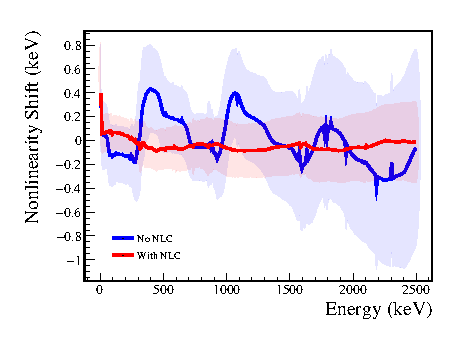
\includegraphics[width=0.8\linewidth]{DigitizerNonlinearity}
  \caption[Measured Digitizer Nonlinearity vs Energy]{\label{fig:dignonlin}
    Digitizer nonlinearity before (red) and after (blue) being corrected. This nonlinearity is measured by comparing the energy measured in the high gain channel to that of the low gain channel.
  }
\end{figure}
The efficiency of each of the sum and coincident energy cuts can be evaluated by computing the ratio of simulated \bbes\ events that pass the cut to the total number of simulated events.
The primary source of uncertainty arises from imperfections in the simulated \bbes\ spectra produced by \texttt{DECAY0} (see Section~\ref{sec:essims}).
Additionaly uncertainty in the spectral shape arises from energy nonlinearity.
Since the efficiency is calculated by integrating over portions of the coincidence spectrum, an upper limit on the systematic error can be found using the KS statistic of a comparison between the simulated spectrum and the true spectrum.
As discussed in Section~\ref{sec:decay0vskandi}, we can perform this comparison by using the Kotila and Iachello spectrum as a proxy.
This relies on the assumption that the Kotila and Iachello spectrum has corrected the dominant errors in the \texttt{DECAY0} spectrum; if any errors coexist in both spectra that have a similar order of magnitude, then this approach will underestimate the uncertainty.
To account for energy nonlinearity, each simulated energy is shifted to represent the effects of digitizer nonlinearity and energy drift.
Digitizer nonlinearity originates from the fact that some digitizer energy bins are slightly wider than others and has an approximately sawtooth dependency on energy with a period of ${\sim}600$~keV.
A correction is applied that reduces the size of this nonlinearity to ${\sim}0.1$~keV in magnitude and smooths it out significantly, as shown in Figure~\ref{fig:dignonlin}.
Digitizer nonlinearity is included in the simulation by shifting each energy according to a sawtooth function with rms 0.1~keV and period 600~keV:
\begin{equation}
  \Delta(E) = \sqrt{3}\cdot (0.1~\mathrm{keV}) \big(\mathrm{rem}(\frac{E-150~\mathrm{keV}}{600~\mathrm{keV}}) \big)
\end{equation}
where $\mathrm{rem}$ is the remainder function as defined in the \cpp standard library.
An additional shift that is randomly sampled from a Gaussian distribution with standard deviation $0.00015\cdot E$ is applied to simulate the effect of gain drift, based on the drift observed during DS5.
After applying both of these alterations to the \texttt{DECAY0} spectrum, a KS test is performed against the Kotila and Iachello spectrum, and a maximum CDF difference of 0.08\% is observed, as shown in Figure~\ref{fig:decay0NLCks}.
This difference is used as an upper limit on the uncertainty from the energy range cuts for \tnbb\ modes.
\begin{figure}[h]
  \centering
  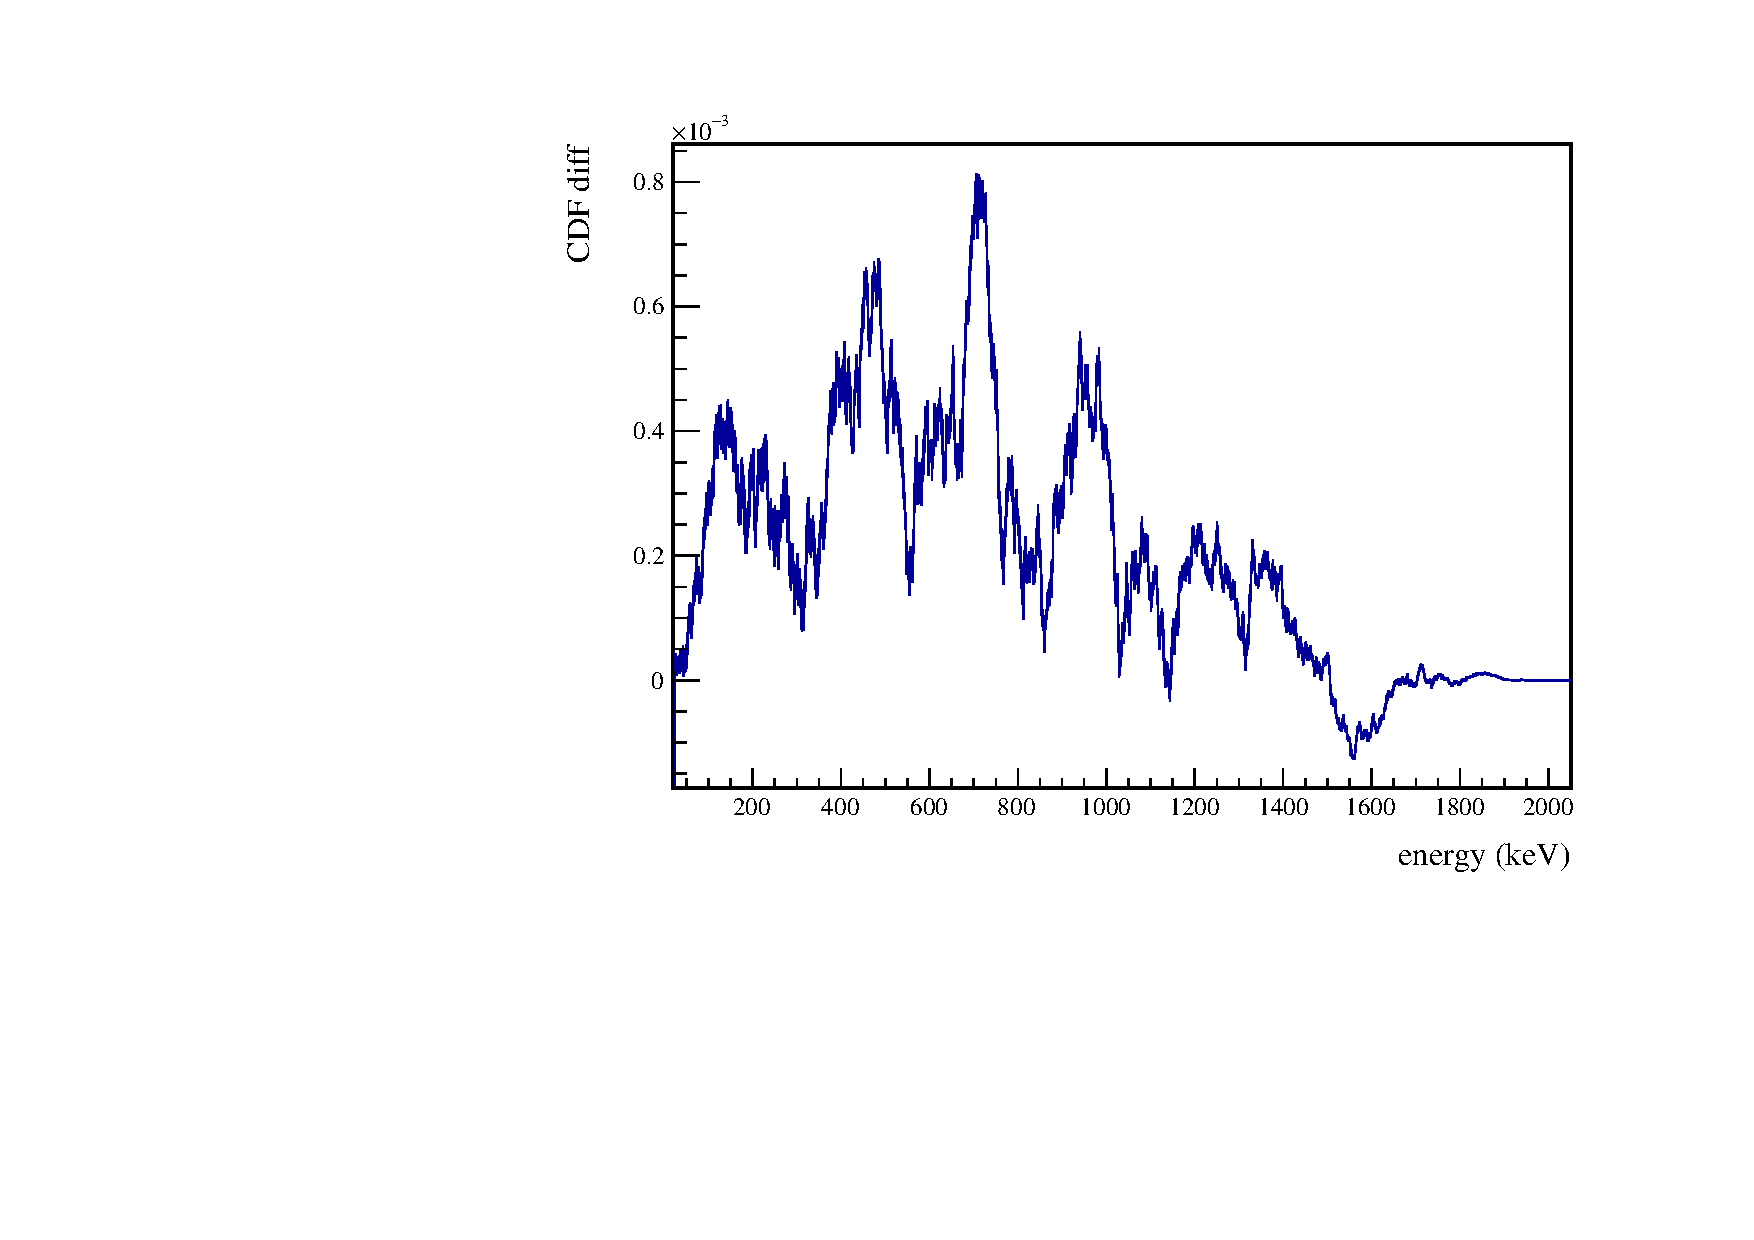
\includegraphics[width=0.6\linewidth]{decay0KS}
  \caption[KS Test of decay0 spectrum with energy non-linearities vs Iachello spectrum]{\label{fig:decay0NLCks}
    KS test comparing the CDFs of the simulated \texttt{DECAY0} \tnbb\ ground state decay with energy nonlinearity modifications applied to the Kotila and Iachello simulated spectrum.
  }
\end{figure}

For \znbb, the energy ranges selected by this cut surround peaks corresponding to the \Qbb s of the decay modes or sum peaks of the \Qbb\ with a deexcitation $\gamma$.
In this case, since we are no longer integrating over a \bb -spectrum, the uncertainty in the efficiency will depend on shifts in the peak, similar to the ROI-efficiency.
Since the energy regions selected keep at least 99.9\% of these peaks in all cases, we can set an upper limit on the uncertainty by checking the ROI efficiency uncertainty around the 2039~keV \Qbb, assuming an ROI tuned to select 99.9\% of the peak.
The uncertainty observed in this case is 0.325\%, which is applied to the energy range cuts for \znbb\ modes.
For both \znbb\ and \tnbb\ modes, this efficiency uncertainty is sub-dominant, so these highly conservative uncertainty estimates will suffice.

\subsection{Muon Veto Cut}
\begin{figure}
  \centering
  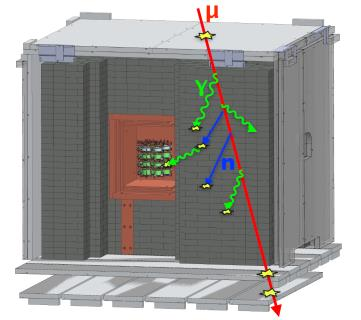
\includegraphics[width=0.7\textwidth]{muonevent}
  \caption[Example muon event]{\label{fig:muonevent}
    A cartoon of a particle shower created by a muon event. The particles produced in such a shower can hit multiple detectors, producing multi-detector events.
  }
\end{figure}
Cosmic ray muons have the potential to produce partical showers in the \MJD\ that can produce \msmd\ events and can activate short-lived isotopes that in turn may decay, producing delayed \msmd\ events.
Background events caused by muons can be cut using the muon veto system.
This analysis follows the standard \MJD\ muon cut procedure, for which any HPGe detector events occurring 20~ms before and 1~s after a tagged muon event are cut.
This cut will remove $>99.9$\% of events induced by the muon shower, based on simulations\cite{2015wiseman}.
In reality, the cut efficiency is slightly lower due to periods of time where the muon veto system clock became desynchronized with the Germanium detector clock.
The impact of this cut is to reduce the total livetime in each module by $<40$~s per day\cite{2015wiseman}.

\section{Combined Detection Efficiency for \bbes}
The final efficiency measurement combining all of the effects described in this chapter for each \bbes\ mode is measured directly from the simulations by computing the ratio of events that survive all cuts and effects to the total number of generated events.
The efficiency used is the exposure-weighted average of the simulated efficiency for each subdataset.
Because each module is an independent measurement, separate efficiencies are measured for modules~1 and~2.
Because of correlations causing the probability of certain effects causing sacrifice of a \bbes\ event to be conditional on other effects, the combined efficiency will differ from simply being the product of the individual efficiencies.
This means that the combined efficiency $\epsilon_{comb}$ for each effect $k$ is:
\begin{equation}
  \epsilon_{comb} = \prod_{k=0}^N P(\mathrm{event~is~cut} | \mathrm{cuts~} 0\dots k-1 \mathrm{~are~applied})
\end{equation}
In spite of this, we will assume that the sources of error are uncorrelated and the fractional uncertainty is independent of what other effects have been applied.
The effect of this assumption will be discussed below.
This implies that the uncertainty on the combined efficiency, $\sigma_{\epsilon,comb}$ can be expressed as:
\begin{equation}
  \sigma_{\epsilon,comb}=\epsilon_{comb} \sqrt{ \sum_{k=0}{N} (\frac{\sigma_{\epsilon,k}}{\epsilon_k})^2 }
\end{equation}
The values $\epsilon_k$ represent the probability of cutting an event assuming no other analysis cuts are applied.
Because of correlations among the cuts (particularly between the sum and coincident energy cuts), this results in a double-counting of uncertainty, making this a conservative estimate.

Table~\ref{tab:eff_2vBB_0_1} shows the efficiency for each effect described in this chapter and uncertainty on each efficiency, and the combined efficiency and uncertainty.
\begin{table}[h]
  \centering
  ../../appAllResults/tables/table_2vBB_ES0_1_efficiency.tex
  \caption[Detection efficiency summary for \tnbb\ to the \SP{0}{+}{1} state of \Se{76}]{\label{tab:eff_2vBB_0_1}
    Table of detection efficiencies and uncertainties for \tnbb\ of \Ge{76} to the \SP{0}{+}{1} state of \Se{76}. Efficiencies of individual effects are calculated without applying other cuts; because of correlations between cuts (especially the sum and coincident energy cuts), simply multiplying these efficiencies together will underestimate the efficiency. The final efficiency calculated here correctly accounts for such correlations. Note that the efficiencies are the combined efficiency for the 559 and 563~keV peaks.
  }
\end{table}
Similar tables for each other \bbes\ peak are shown in Appendix~\ref{app:allresults}.
In all cases the dominant uncertainties come from either the dead layer thickness or the simulation uncertainty.
Figure~\ref{fig:escuteffects} shows the effect of each cut as it is applied sequentially to the \tnbb\ to \SP{0}{+}{1} peaks.
\begin{figure}[htb]
  \centering
  \includegraphics[width=0.8\textwidth]{ESAllcuts}
  \caption[Simulated \tnbb\ to \SP{0}{+}{1} peaks with cuts applied]{\label{fig:escuteffects}
    The 559~and 563~keV peaks from the \tnbb\ decay to the \SP{0}{+}{1} decay mode, with the effect of all cuts applied sequentially to simulated ES events. The cuts are applied from top to bottom (i.e.~red, blue, then green). Many events will be cut by more than one of these; in that case it will be colored by whichever cut is applied first. 
  }
\end{figure}




\section{Double Beta Decay to Excited States Results}
Now that we have found and characterized a specific detection signature for each decay mode, we can apply this search to data.
This result will look at open runs from datasets 1~through 6a that were designated silver or gold in run quality.
The duty cycle and changes that define each data set are shown in Figure~\ref{fig:dutycycle}.
These were taken from January~12, 2016 to April~18, 2018, and contain a total of 13.4~kg~y of isotopic exposure for module~1 and 7.9~kg~y for module~2.
Approximately half the data in these datasets is blinded, and is not included in this analysis.
The \MJD\ uses a statistical blinding scheme in which 3/4 of runs are blinded administratively (i.e.~through file access) in cycles of 31~h of unblinded runs followed by 93~h of blinded runs.
Unblinding data proceeds in a staged fashion, where first single-site events, not including any interesting physics regions are unblinded (i.e.~no background ROI, \znbb\ to the ground state ROI, low energy or multi-site data).
This data is used for a variety of data validation checks prior to unblinding of any other data.
The remaining data are separately unblinded after a collaboration review for individual analyses and users.
For this analysis, the multi-site events have been left blinded.

\begin{figure}[h]
  \centering
  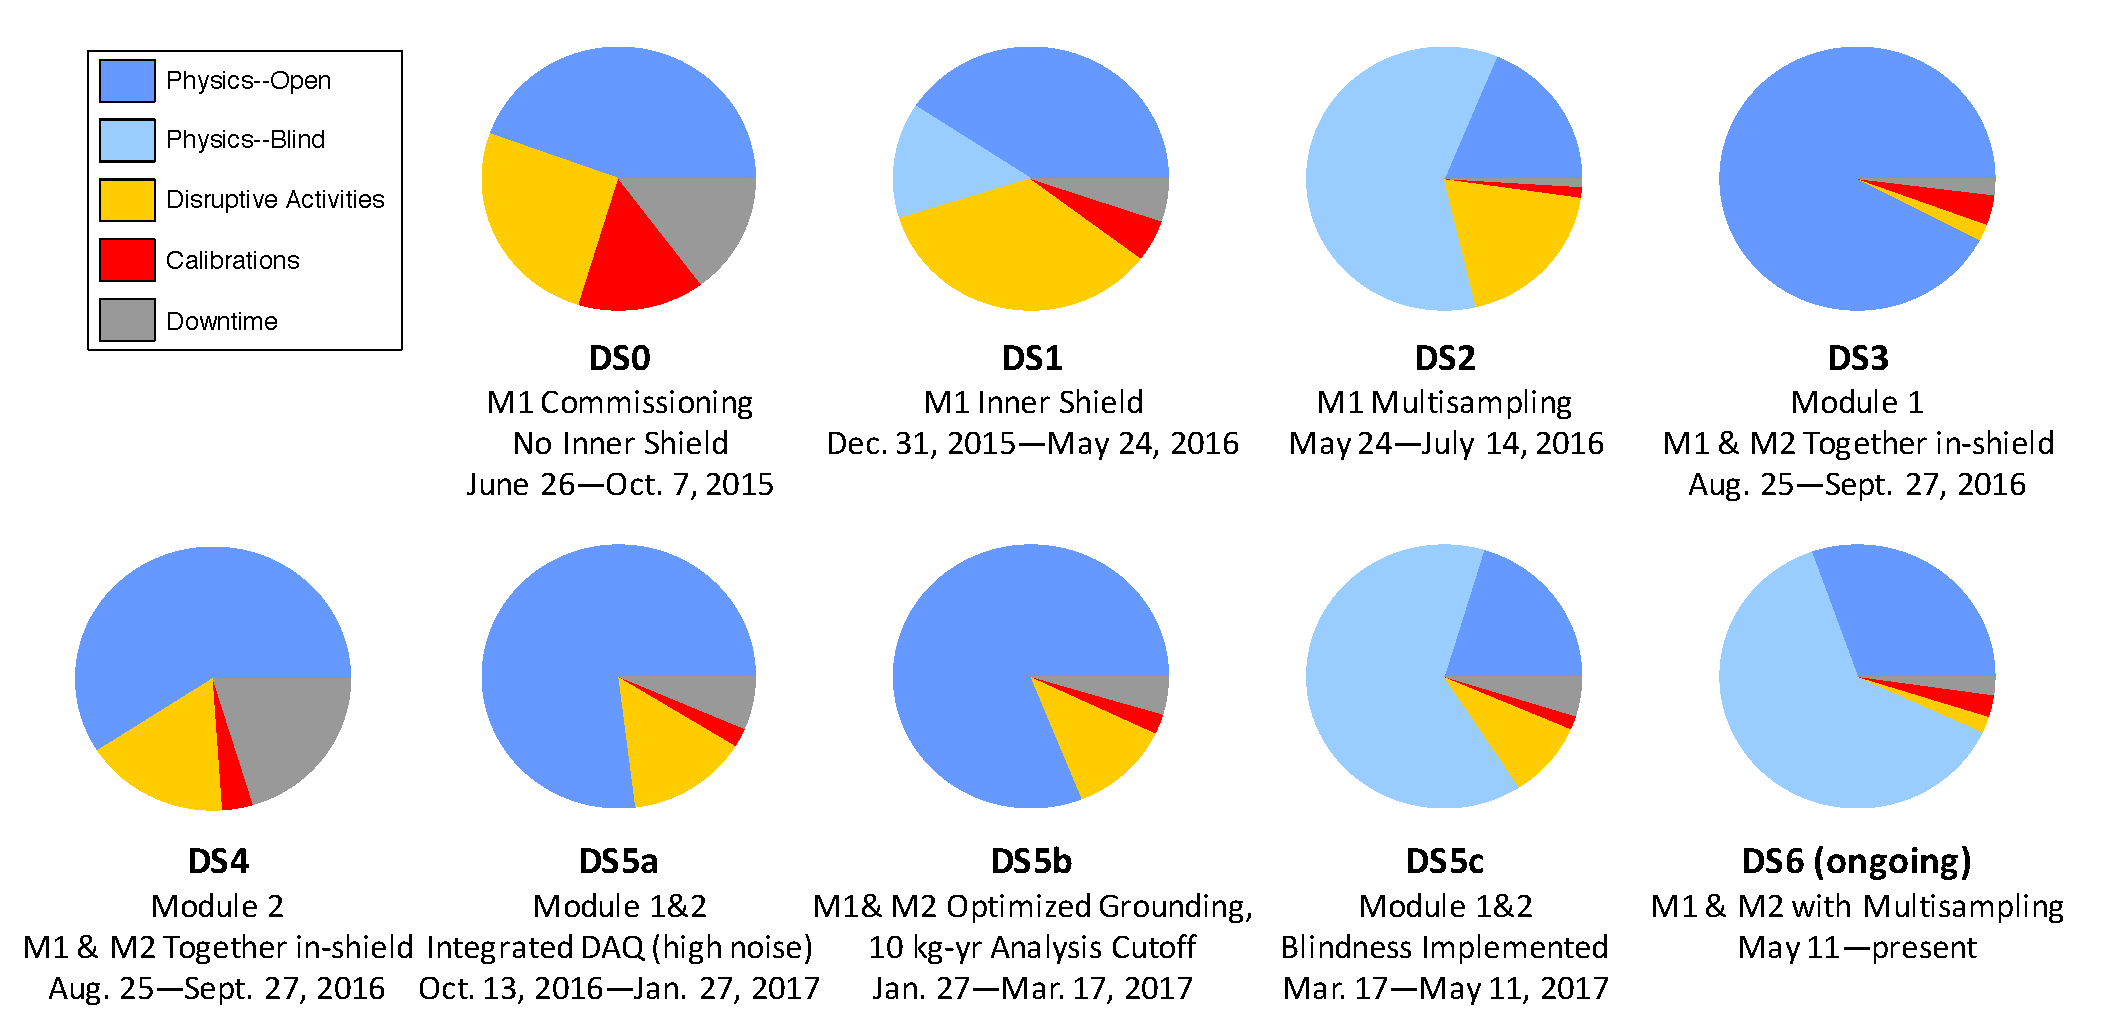
\includegraphics[width=0.9\linewidth]{dutycycle}
  \caption[Dataset and Duty Cycle Summary]{\label{fig:dutycycle}
    The duty cycles for each major dataset used in this analysis, and a brief discription of the major changes in configuration that define each data set.
  }
\end{figure}

In the open multi-site data, 5558 multi-detector events were observed.
A histogram of the event multiplicities is shown in Figure~\ref{fig:datamult}, and a spectrum of all multiplicity~2 event energies is shown in Figure~\ref{fig:data2D}.
\begin{figure}[h]
  \centering
  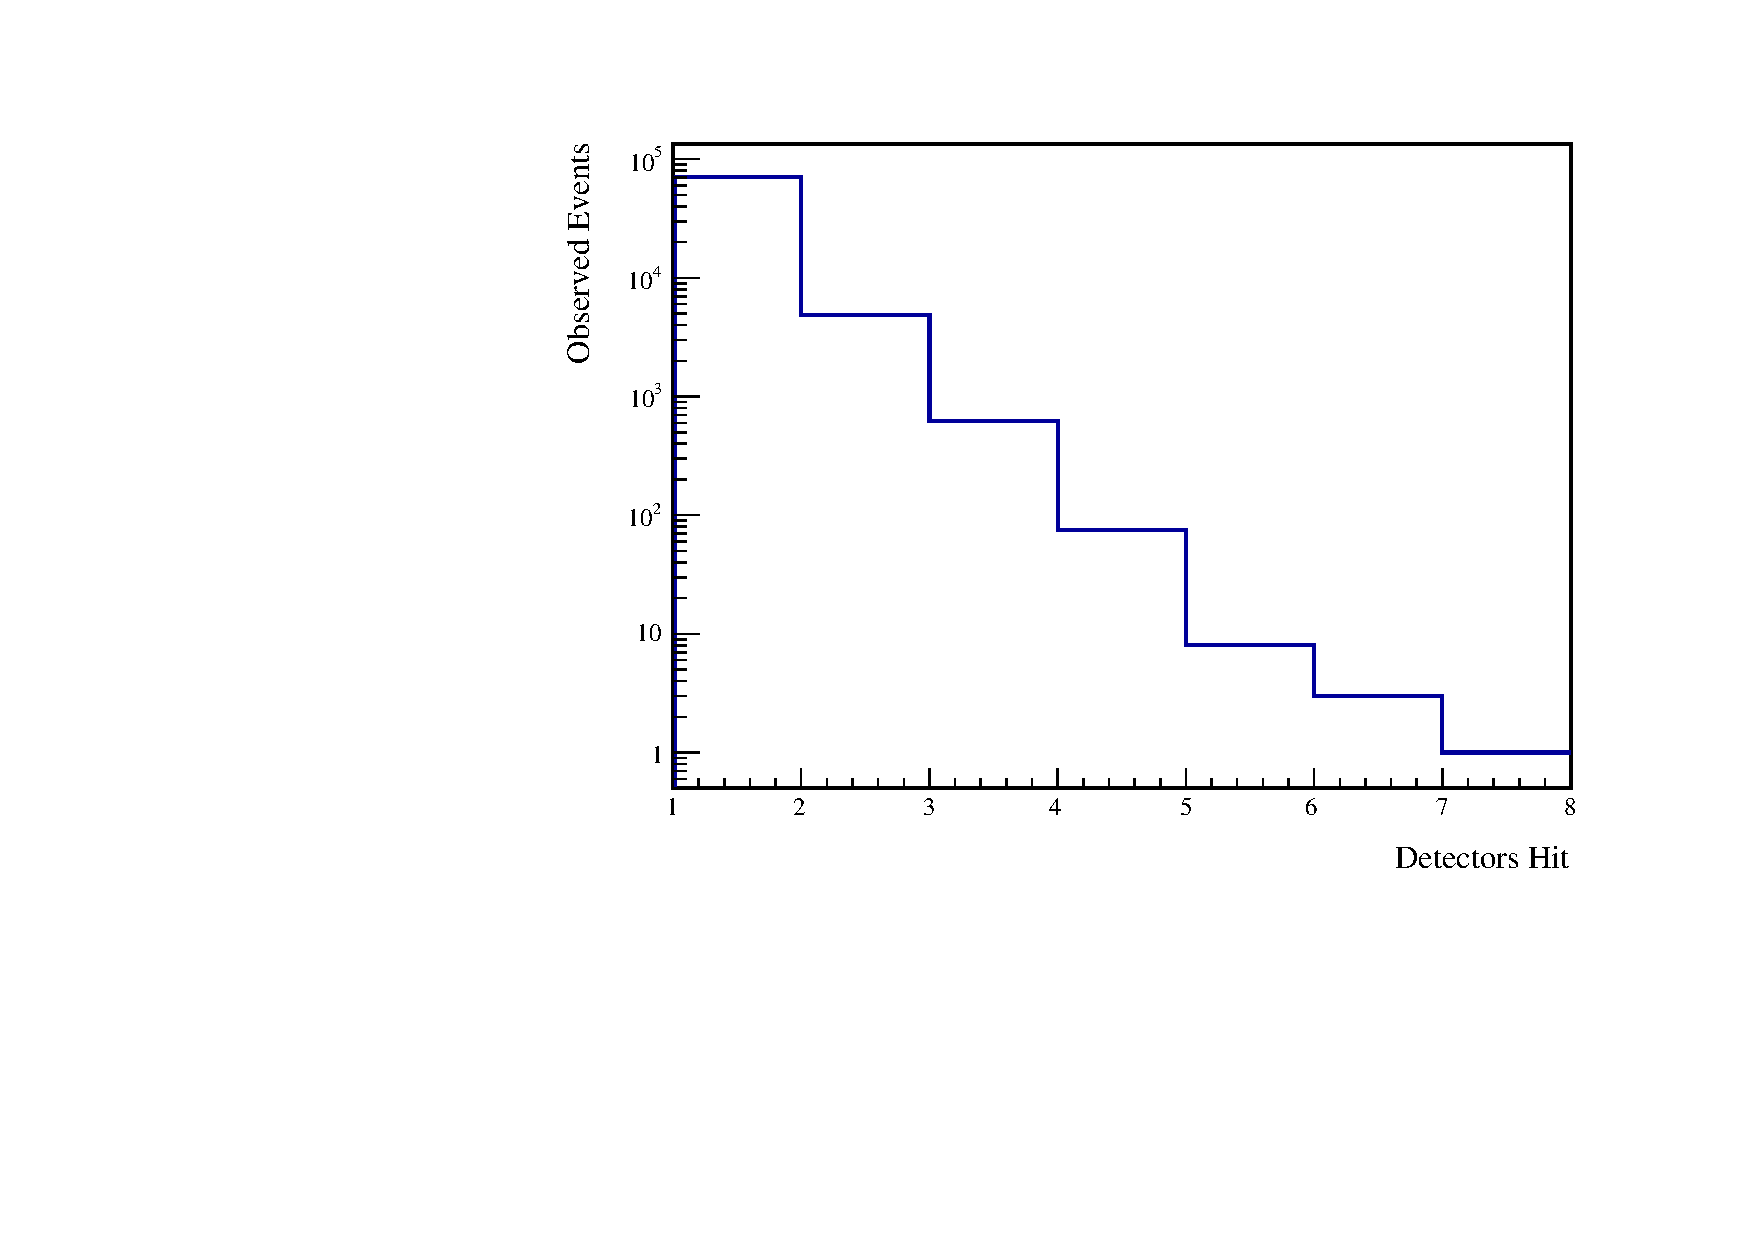
\includegraphics[width=.6\linewidth]{DataMultiplicity}
  \caption[Measured event multiplicities]{\label{fig:datamult}
    The measured multiplicities for events in datasets~1-6a. For multiplicity~1 events, only events with energy between 40~keV and 4~MeV were considered.
  }
\end{figure}
\begin{figure}[h]
  \centering
  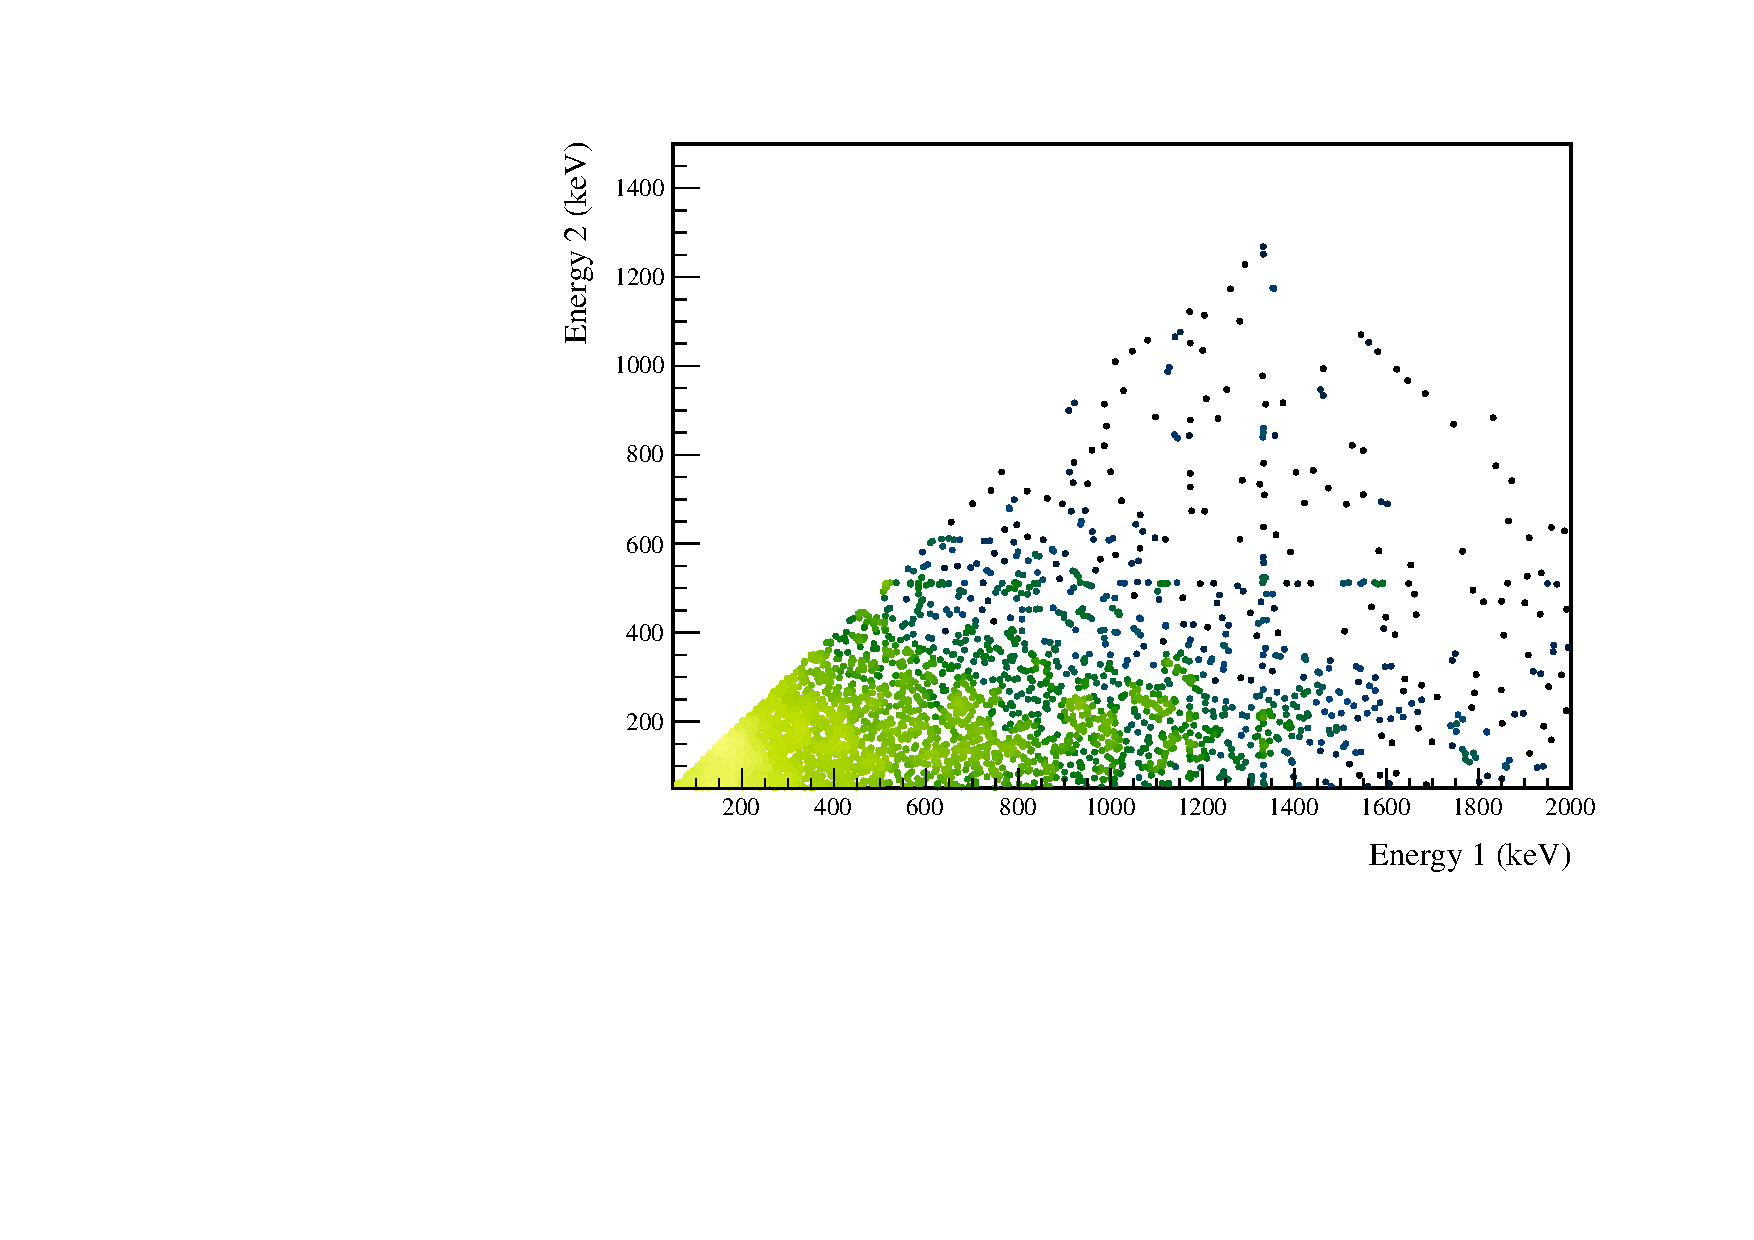
\includegraphics[width=.8\linewidth]{Data2D}
  \caption[Measured energy spectrum of multiplicity~2 events]{\label{fig:data2D}
    Measured energy spectrum of open multiplicity~2 events in datasets~1-6a.
  }
\end{figure}

\section{Validation}
In addition to the basic run selection and data cleaning validation checks that are run on all multiplicity~1 data, we perform some additional checks on high multiplicity data.
As previously, this section will describe these checks applied to the \tnbb\ to the \SP{0}{+}{1} state of \Se{76}.
Similar checks are performed on other decay modes in Appendix~\ref{app:allresults}.

\subsection{Data Rate} \label{sec:ratecheck}
Any spikes in the rate of multi-site events would potentially indicate problems with run selection or data cleaning.
Significant variation in the data rate is expected due to changes in which detectors are active.
For this reason, the rate of multi-site events with respect to the sensitive exposure, defined as the exposure times the detection efficiency of \bbes\ events, is used instead.
This quantity is interesting because the rate of observed \bbes\ events should be constant with respect to it.
The changes in detection efficiency from one subdataset to another for both backgrounds and \bbes\ are highly correlated and driven by which detectors are enabled.
For this reason, we can reasonably expect that the backgrounds should also have a nearly constant rate with respect to sensitive exposure, although differences between background source positions and the distribution of \Ge{76} in the detectors imply that some differences should be expected.
Figure~\ref{fig:eventrate} indeed shows a slow reduction in the overall background rate over time.
One possible explanation for this is that a significant quantity of \Ge{68} exists in natural HPGe detectors as a result of cosmogenic activation, and has a half-life of 271~days, which is observable on the timescale of the \MJD's operation.
\iso{68}{Ga} is a $\beta^+$ emitter which is a part of the \Ge{68} decay chain, which produces two 511~keV $\gamma$s and has a high probability of producing multi-detector events.
\begin{figure}[ht]
  \centering
  \subfloat{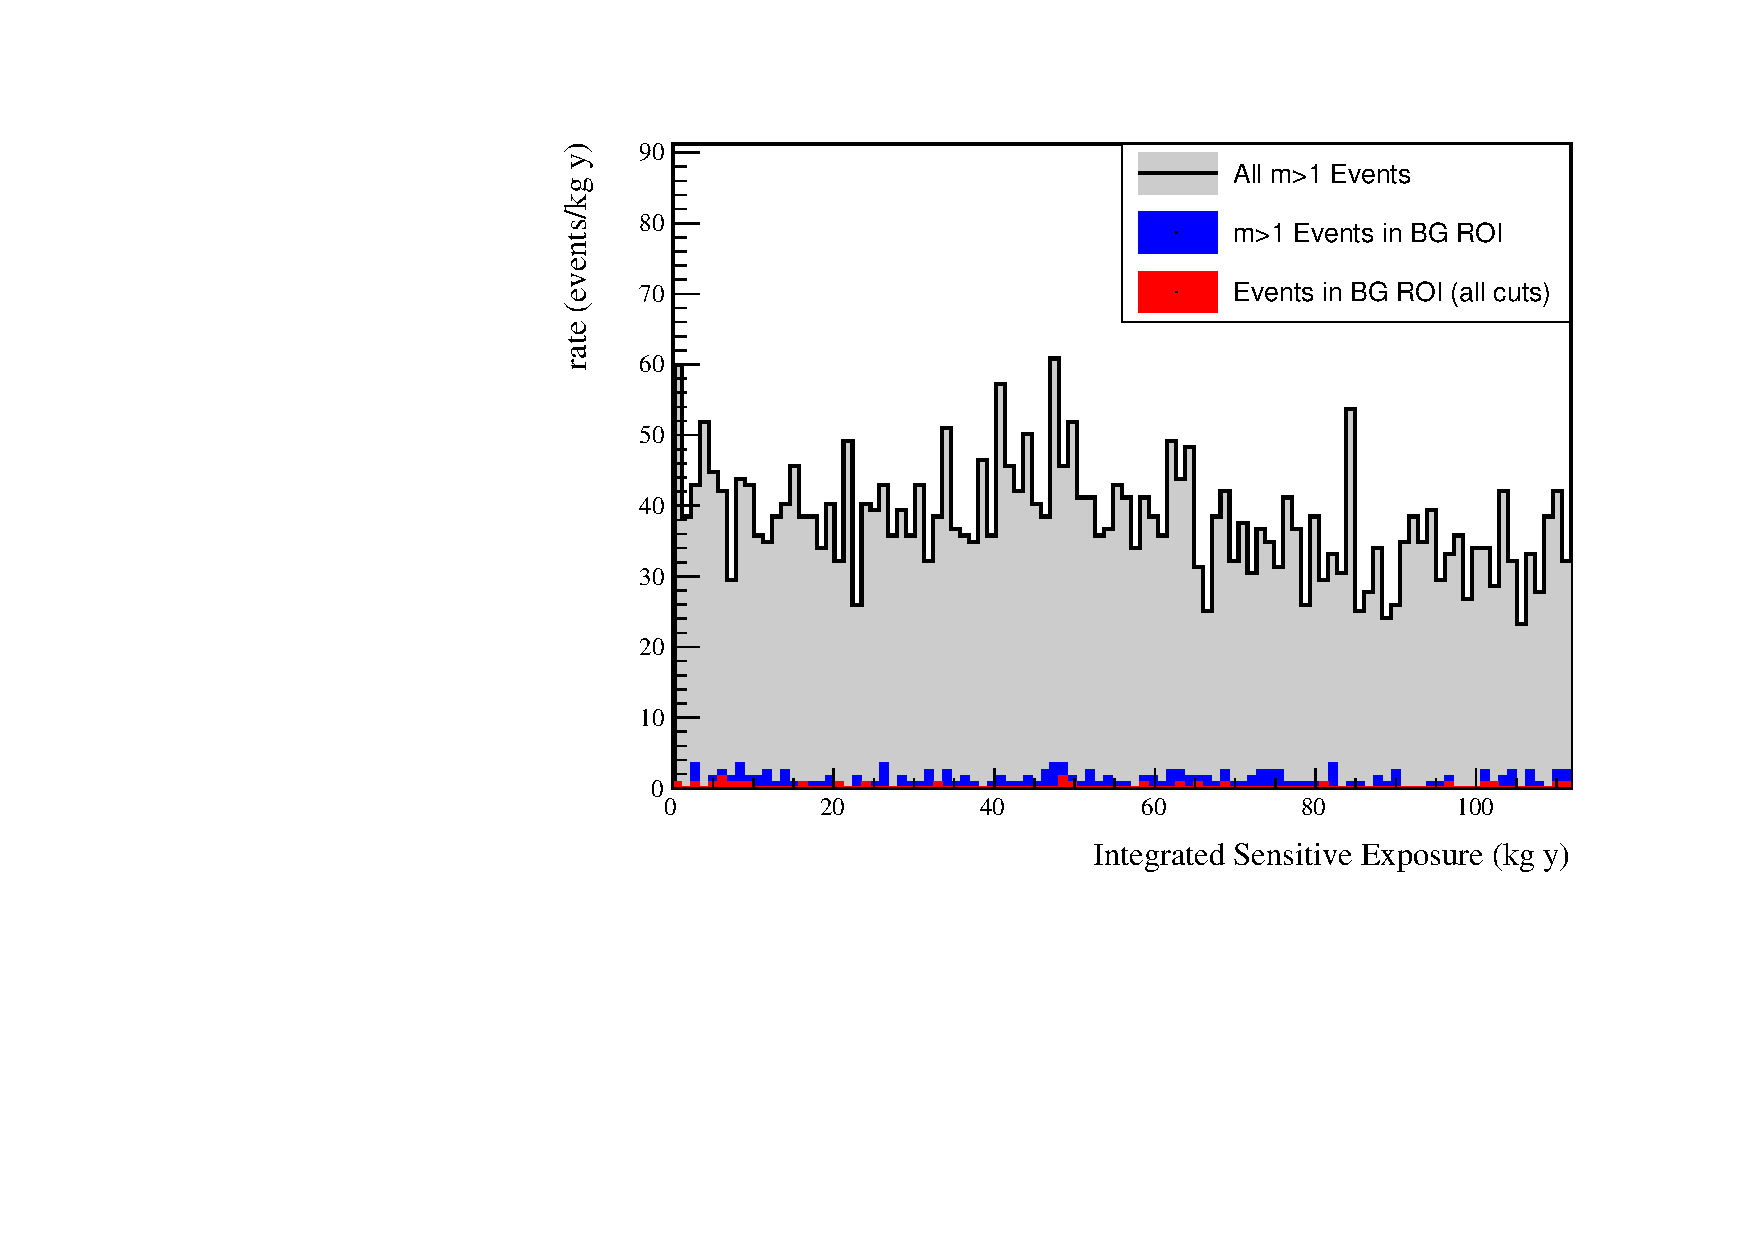
\includegraphics[width=.5\linewidth]{M1datarate}}
  \subfloat{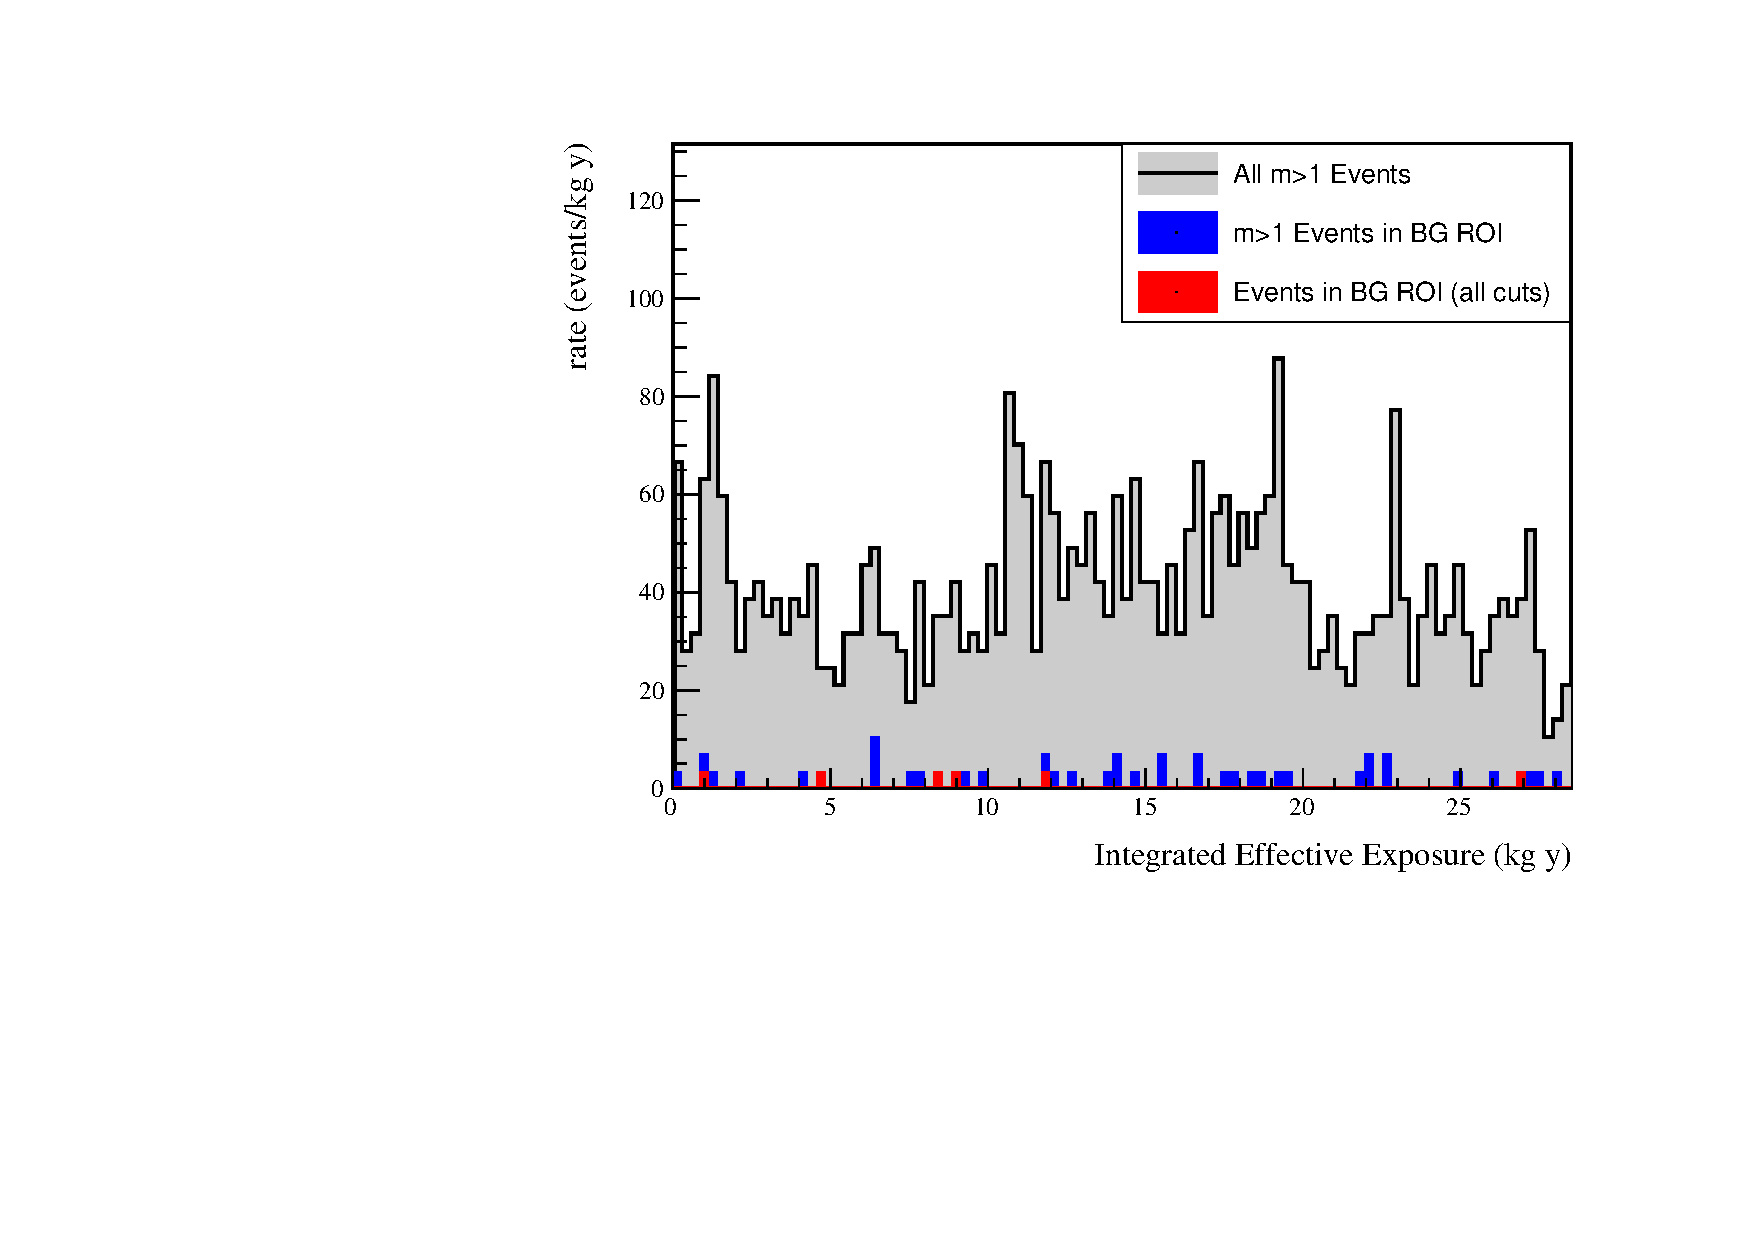
\includegraphics[width=.5\linewidth]{M2datarate}}
  \caption{\label{fig:eventrate}
    Event rate with respect to sensitive exposure, or the detection efficiency of the \tnbb\ decay to the \SP{0}{+}{1} excited state times the exposure. Integrated exposure is the total sensitive exposure prior to an event. The background rate is expected to be mostly flat, with differences discussed in Section~\ref{sec:ratecheck}.
  }
\end{figure}


\subsection{Background Cut Evaluation} \label{sec:bgcuteval}
A second important check to ensure that the cuts applied to each \bbes\ mode is to compare each cut efficiency to the expected background cut efficiency.
Since the background model used for this analysis uses preliminary results, disagreement between the expected and measured cut efficiencies could indicate a difference between the background model and the measured backgrounds rather than a problem with the application of cuts.
However, any major discrepencies could indicate a bug in the analysis.
To perform this comparison, the cut efficiencies are measured both in terms of the total number of events cut, $\epsilon_{total}$ and the number of events that are uniquely cut, $\epsilon_{unique}$ (i.e.~not cut by any of the others).
Table~\ref{tab:bgcutstable} lists each cut for the \bbes\ decay to the \SP{0}{+}{1} state and the expected and measured cut efficiencies.
The expected background cut efficiencies, $\langle\epsilon\rangle$ represent the fraction of simulated events cut, measured as an exposure-weighted average across all open datasets.
The measured background cut efficiencies, $\hat{\epsilon}$ represent the measured fraction of events cut.
Statistical uncertainties in the expected efficiencies are negligible compared to the uncertainties in the measured efficiencies, and are not included.
The sacrifice is the number of events uniquely sacrificed by the cut.
$\Delta \mathrm{DP}$ is the expected improvement in discovery potential, defined in Appendix~\ref{app:sens}, as a result of the cut.
Figure~\ref{fig:datacuts2D} shows the effects of data cuts on multiplicity~2 events.
Figure~\ref{fig:cutsroi} shows the effects of cuts on events in the ROI in both measured and simulated data.

\begin{figure}
  \centering
  \includegraphics[width=0.8\linewidth]{Data2Dcuts}
  \caption[Effect of data cuts on measured multiplicity 2 events]{\label{fig:datacuts2D}
    Energy spectrum of multiplicity~2 events. Red events are events that are cut. For blue events, at least one of the hits passes all cuts; however, the other hit may fail. For green events, one of the hits must both pass all cuts and place the event in the BG or ES ROI. Note that the green events include any events of multiplicity $>1$; for higher multiplicity events, instead of showing the energy in the second detector, the sum of the energy in all other detectors is shown.
  }
\end{figure}

\begin{figure}
  \centering
  \subfloat{\includegraphics[width=0.5\linewidth]{DataAllCuts}}
  \subfloat{\includegraphics[width=0.5\linewidth]{BGAllCuts}}
  \caption{\label{fig:cutsroi}
    Effect of cuts on all events in the BG and ES ROIs. Events are applied in sequence from top to bottom, meaning that if an event is cut by multiple cuts, it will be colored based on the first cut that applied. Both the simulated and measured event spectra are shown for comparison.
  }
\end{figure}

\begin{sidewaystable}[p]
  \centering
  ../../appAllResults/tables/table_2vBB_ES0_1_bgcuts.tex
  \caption[Detection efficiency summary for \tnbb\ to the \SP{0}{+}{1} state of \Se{76}]{\label{tab:bgcutstable}
    Table of detection efficiencies and uncertainties for \tnbb\ of \Ge{76} to the \SP{0}{+}{1} state of \Se{76}.
  }
\end{sidewaystable}

\section{Results}


\subsection{Statistical Methods}
Neyman confidence intervals are computed for each peak in each \bbes\ decay mode, and each module.
For a given peak $k$, the expected number of signal counts is
\begin{equation}
  \langle s_k\rangle = \ln2 \frac{N_A}{m_{76}}\epsilon_k\frac{M_{iso}T_{live}}{T_{1/2}}
\end{equation}
where $M_{iso}$ is the total isotopic mass and $T_{live}$ is the livetime ($M_{iso}T_{live}$ is the exposure and is calculated in Section~\ref{sec:sds} to be $13.356\pm0.021$~kg-y for module~1 and $7.872\pm0.13$~kg-y for module~2.
$\epsilon_k$ is the total detection efficiency of the decay mode using peak $k$, which can be found in Appendix~\ref{app:allresults}.
$m_{76}=0.0759214$~kg is the molar mass of \Ge{76}, and $N_A=6.02214076\times10^{23}$ is Avagadro's number.
Fun fact: an Avagadro's number of avocados has approximately the volume of Mars.
We will define the single count half-life to be
\begin{equation}
  T^*_k=\ln2 \frac{N_A}{m_{76}}\epsilon_kM_{iso}T_{live}
\end{equation}
which is the decay half-life that would produce on average one count in signal ROI $k$.

Because of the nearly background free nature of this search, a likelihood construction is used that assumes Poisson statistics for the number of counts in the signal and background ROIs.
\begin{equation}
  \label{eq:rolke}
  \begin{aligned}
    \mathcal{L}_k(T_{1/2},T^*_k,b_k|n_k,m_k,\langle T^*_k\rangle, \sigma_{T^*,k},\tau)
    &=\frac{\mu_k^{n_k}e^{-\mu_k}}{n_k!} \cdot \frac{(b_k\tau)^{m_k}e^{-b_k/\tau}}{m_k!} \cdot
    \frac{1}{\sigma_{T^*,k}\sqrt{2\pi}}e^{-\frac{(T^*_k-\langle T^*_k\rangle)^2}{2\sigma_{T^*,k}^2}} \\
    \mu_k &= s_k+b_k = \frac{T^*_k}{T_{1/2}} + b_k
  \end{aligned}
\end{equation}
$T_{1/2}$ represents the decay mode half-life and is the parameter of interest.
$T^*_k$ and $b_k$ are nuisance parameters representing the measured single count halflife and expected backgrounds in the ES ROI, respectively.
$\mu_k$ is the total expected number of counts, combining background and signal, in the ES ROI.
$n_k$ is the measured number of events in the ES ROI and is expected to be drawn from a Poisson distribution with mean $\mu_k$.
$m_k$ is the measured number of events in the BG ROI and is expected to be drawn from a Poisson distribution with mean $b_k/\tau$, where $\tau$ is the ratio between the number of expected background counts in the BG ROI to the number in the ES ROI.
Note that since these events are multi-detector events, it is possible for multiple hits in the event to fall into one of the ROIs; however, we will choose a single hit to represent the whole event.
In this case, any hit that falls into the ES ROI takes precedence over any hit that falls into the BG ROI, and if multiple hits fall into the ES ROI, one is chosen at random.
This approach would produce a very small bump in an otherwise flat background at the ES ROI; this is accounted for in the calculation of $\tau$.
$\tau$ is usually determined based on the background simulation; however, in cases where the simulation statistics are limited after applying all cuts, a flat background is assumed and the ratio of the ES ROI width to the BG ROI width is used.
$\langle T^*_k\rangle$ represents the expected value of $T^*_k$ based on previous measurements of exposure and detection efficiency, which is assumed to have Gaussian uncertainty:
\begin{equation}
  \sigma_{T^*,k} = \langle T^*_k\rangle\sqrt{(\frac{\sigma_{\epsilon,k}}{\epsilon_k })^2 + (\frac{\sigma_{exposure}}{M_{iso}T_{live} })^2}
\end{equation}
The implementation of Equation~\ref{eq:rolke} is performed by the \texttt{TRolke} class in ROOT \cite{rolke2005}.
This likelihood function is used to compute a likelihood ratio
\begin{equation}
  \mathrm{LR}_k(T_{1/2}) = \frac{\mathrm{sup}_{T^*_k,b_k}\left(\mathcal{L}_k(T_{1/2},T^*_k,b_k|n_k,m_k,\langle T^*_k\rangle, \sigma_{T^*,k},\tau)\right)}{\mathrm{sup}_{T_{1/2},T^*_k,b_k}\left(\mathcal{L}_k(T_{1/2},T^*_k,b_k|n_k,m_k,\langle T^*_k\rangle, \sigma_{T^*,k},\tau)\right)}
\end{equation}
The \texttt{TRolke} class analytically computes the supremum over $T^*_k$ and $b_k$, returning the log-likelihood difference.
The implementation is parameterized in terms of $\Gamma=\frac{1}{T_{1/2}}$, which is restricted to positive values; if the supremum of the function has a negative value of $\Gamma$, then the value at $\Gamma=0$ is used instead.
Since the likelihood ratio is expected to be $\chi^2$-distributed, to construct a 90\% confidence interval, we seek the values of $T_{1/2}$ corresponding to a log-likelihood ratio value of 2.7.
In cases where the lower limit on $\gamma$ is found to be $<0$, a lower limit on $T_{1/2}$ is reported.

After constructing confidence intervals for each peak and module individually, a combined confidence interval is constructed for each \bbes\ decay mode.
A combined log-likelihood over all peak/module combinations $k$ is defined by
\begin{equation}
  \mathrm{log}\left(\mathcal{L}(T_{1/2})\right) = \sum_{k=0}^{N} \mathrm{sup}_{T^*_k,b_k}\left(\mathrm{log}\left(\mathcal{L}_k(T_{1/2},T^*_k,b_k|n_k,m_k,\langle T^*_k\rangle, \sigma_{T^*,k},\tau)\right)\right)
\end{equation}
This construction relies on the fact that the $T^*_k$ and $b_k$ values across each peak can be independently maximized, enabling the continued use of the \texttt{TRolke} implementation.
A combined likelihood ratio is constructed:
\begin{equation}
  \mathrm{log}\left(\mathrm{LR}(T_{1/2})\right)=\mathrm{log}\left(\mathcal{L}(T_{1/2})\right) - \mathrm{sup}_{T_{1/2}}\left(\mathrm{log}\left(\mathcal{L}(T_{1/2})\right)\right)
\end{equation}
and used to compute a confidence interval as above.
Table~\ref{tab:alllimits} contains the limits constructed for each decay mode, peak and module.
For all modes, a lower half-life limit is set.

Note that each decay mode is analyzed independently.
The problem with this approach is that all decay modes have the 559~keV peak in common, meaning that the results will be correlated.
For this result, since all modes only have a lower limit on half-life set, this approach is not problematic since for any individual mode, we would take the supremum over all other half-lives, which would be at or near infinity, resulting in the same sets of equations used here.
However, if the \bbes\ to the \SP{0}{+}{1} mode is discovered, it will become necessary to perform a full combined analysis.

The detection sensitivity is computed by constructing a toy Monte Carlo for each decay mode, assuming that each $T_{1/2}$ is infinite.
For each sample $i$, a random $n_i$ and $m_i$ is drawn from a Poisson distribution with mean $b_k$ and $m_k$.
The confidence interval for a measurement with these values is computed.
The median sensitivity is extracted by taking the median lower half-life limit over all samples.
For the results in Table~\ref{tab:alllimits}, 100001 samples were used.

\subsection{Limits and Sensitivities}
\begin{figure}[h]
  \centering
  \includegraphics[width=.8\linewidth]{DataROIs}
  \caption[Measured events after all cuts with ROIs drawn]{\label{fig:roievents}
    Events that pass all cuts for the \tnbb\ to \SP{0}{+}{1} decay mode. The ES and BG ROIs are highlighted. Note that these ROIs undergo small variations from dataset to dataset, and the ROIs drawn here are averaged over all datasets. The energies shown in this spectrum are the energies of the hit that places the event in the ROI. A single event will only be placed once into an ROI; however, as drawn here, if multiple hits in a single event fall into an ROI, they will all be drawn.
  }
\end{figure}
The limits and sensitivities for each peak and module individually, and the combination for each mode, are shown in Table~\ref{tab:alllimits}.
Figure~\ref{fig:roievents} shows the event spectrum after all cuts have been applied with both ROIs highlighed.

\begin{table}[h]
  \scriptsize
  \centering
  \begin{tabular}{|c|c|c c c c c|c|c|}
\hline  Decay Mode & Peak & Module & $n_{ROI}$ & $m_{BG}$ & \makecell{Expected\\ROI BGs} & $T^*\,(\times 10^{23} \mathrm{y})$ & \makecell{$T_{1/2}\,(\times 10^{23} \mathrm{y})$ \\ 90\% Limit} & \makecell{$T_{1/2}\,(\times 10^{23} \mathrm{y})$ \\ 90\% Sensitivity} \\
\hline
\multirow{5}{*}{\decaySP{2}{0}{1}} & \multirow{2}{*}{559 keV} & M1 & 2 & 23 & 0.88 & $8.41 \pm 0.60$ & $>1.9$ & $>3.2$ \\
     &      & M2 & 0 & 2 & 0.09 & $2.10 \pm 0.37$ & $>1.5$ & $>1.5$ \\
     & \multirow{2}{*}{563 keV} & M1 & 0 & 23 & 0.97 & $8.42 \pm 0.60$ & $>6.2$ & $>3.2$ \\
     &      & M2 & 0 & 2 & 0.08 & $2.08 \pm 0.37$ & $>1.5$ & $>1.5$ \\
     & Combined &  &  &  &  &  & $>6.8$ & $>7.0$ \\
\hline\multirow{3}{*}{\decaySP{2}{2}{1}} & \multirow{2}{*}{559 keV} & M1 & 0 & 16 & 0.68 & $10.43 \pm 1.04$ & $>7.7$ & $>7.7$ \\
     &      & M2 & 0 & 1 & 0.04 & $2.66 \pm 0.88$ & $>1.8$ & $>1.8$ \\
     & Combined &  &  &  &  &  & $>9.6$ & $>5.3$ \\
\hline\multirow{7}{*}{\decaySP{2}{2}{2}} & \multirow{2}{*}{559 keV} & M1 & 2 & 38 & 1.46 & $7.24 \pm 0.87$ & $>1.8$ & $>2.9$ \\
     &      & M2 & 0 & 5 & 0.22 & $1.89 \pm 0.85$ & $>1.2$ & $>1.2$ \\
     & \multirow{2}{*}{657 keV} & M1 & 1 & 20 & 0.69 & $5.49 \pm 0.70$ & $>1.8$ & $>4.0$ \\
     &      & M2 & 0 & 3 & 0.10 & $1.50 \pm 0.74$ & $>0.9$ & $>0.9$ \\
     & \multirow{2}{*}{1216 keV} & M1 & 0 & 29 & 0.79 & $3.14 \pm 0.84$ & $>2.2$ & $>1.1$ \\
     &      & M2 & 0 & 4 & 0.14 & $0.77 \pm 0.93$ & $>1.1$ & $>1.1$ \\
     & Combined &  &  &  &  &  & $>5.7$ & $>5.3$ \\
\hline\multirow{5}{*}{\decaySP{0}{0}{1}} & \multirow{2}{*}{559 keV} & M1 & 0 & 2 & 0.09 & $11.47 \pm 0.98$ & $>8.4$ & $>8.4$ \\
     &      & M2 & 0 & 0 & 0.00 & $2.92 \pm 0.56$ & $>2.1$ & $>2.1$ \\
     & \multirow{2}{*}{563 keV} & M1 & 0 & 2 & 0.09 & $11.32 \pm 0.96$ & $>8.3$ & $>8.3$ \\
     &      & M2 & 0 & 0 & 0.00 & $2.86 \pm 0.55$ & $>2.1$ & $>2.1$ \\
     & Combined &  &  &  &  &  & $>21.1$ & $>21.1$ \\
\hline\multirow{3}{*}{\decaySP{0}{2}{1}} & \multirow{2}{*}{559 keV} & M1 & 0 & 0 & 0.00 & $12.04 \pm 1.31$ & $>8.8$ & $>8.8$ \\
     &      & M2 & 0 & 0 & 0.00 & $3.01 \pm 1.02$ & $>2.0$ & $>2.0$ \\
     & Combined &  &  &  &  &  & $>11.0$ & $>11.0$ \\
\hline\multirow{7}{*}{\decaySP{0}{2}{2}} & \multirow{2}{*}{559 keV} & M1 & 0 & 2 & 0.08 & $7.16 \pm 0.95$ & $>5.2$ & $>5.2$ \\
     &      & M2 & 0 & 0 & 0.00 & $1.81 \pm 0.85$ & $>1.1$ & $>1.1$ \\
     & \multirow{2}{*}{657 keV} & M1 & 0 & 7 & 0.27 & $7.00 \pm 0.96$ & $>5.1$ & $>5.1$ \\
     &      & M2 & 0 & 1 & 0.02 & $1.76 \pm 0.90$ & $>1.0$ & $>1.0$ \\
     & \multirow{2}{*}{1216 keV} & M1 & 0 & 0 & 0.00 & $3.23 \pm 0.85$ & $>2.3$ & $>2.3$ \\
     &      & M2 & 0 & 0 & 0.00 & $0.81 \pm 0.95$ & $>0.2$ & $>0.2$ \\
     & Combined &  &  &  &  &  & $>16.0$ & $>16.0$ \\
\hline\end{tabular}

  \caption[Final results for all decay modes]{ \label{tab:alllimits}
    Results for all decay modes.
  }
\end{table}

\section{Unblinding Plan}
The result presented in this document uses only open data from DS1-6a.
Data is blinded by administratively by forbidding access to built and gatified files to users; access to blinded data is provided through skim files.
Unblinding proceeds in multiple stages; skim files produced in the first stage exclude high multiplicity events, events in the 400~keV ROI around \Qbb, and low energy events.
Access to these events is provided individually to analyzers through inclusion in skim files accessible only by that individual.
For this analysis, high multiplicity events will be needed.

Prior to unblinding, several steps will be completed.
First, subdatasets must be identified using \texttt{es\_get\_datasets}, requiring access to channel selection files that are produced during the first stage of unblinding.
Next, the live time must be measured. Unfortunately, this requires access to detailed run information from built files, which are left blinded; as a result, \texttt{es\_livetime} must be run by someone with access to the mjd account.
Next, background model and excited state simulations for each subdataset will be produced using \texttt{es\_skimsim}.
Next, cut optimization must be performed using \texttt{es\_optimize\_cuts}.
Because an estimate of a scaling required to get the actual background level from the simulations is required for this step, an estimate should be made using the already unblinded single-site events.
Finally, cuts should be applied with \texttt{es\_apply\_cuts}, and the efficiencies and exposures estimated using \texttt{es\_get\_result} with the \texttt{--nodata} option.
In addition to running this code, plots of the simulated data should be made, similar to those displayed in Appendix~\ref{app:allresults}.
Once this is completed, the plots and efficiencies should be inspected; any discrepancies between the unblinded result and these blinded numbers should be understood prior to unblinding.

Once the analysis is approved for unblinding and skim files with high multiplicity data have been produced, \texttt{es\_skim\_data} will be used to collect the high multiplicity events therein.
\texttt{es\_get\_result} should be run using this data.
The sanity checks discussed in Sections~\ref{sec:ratecheck} and~\ref{sec:bgcuteval} should be performed, and any discrepancies in the data rate or cut efficiencies should be explained, and any changes to the analysis resulting from these checks must be carefully documented.
Finally, \texttt{es\_get\_limits} can be run to get the final limits.

Unblinding will approximately double the exposure to $\sim$40~kg-y of isotopic exposure. Assuming identical backgrounds and efficiencies, the projected half-life sensitivity for the search to the first $0^+$ decay is $\sim1\cdot10^{24}$~yr. It should be noted that rerunning the cut optimization with a more exposure will result in a slightly more stringent set of cuts; as a result, the background rate and detection efficiency will both be lower.
The cutoff at the end of DS6a is motivated by the fact that this encompasses all data in the \MJD\ 2018 \znbb\ release, and has been extensively vetted.
In concert with the next major \znbb\ release, containing DS6b and 6c data, this analysis will add the additional exposure as well.

\bibliographystyle{unsrt}
\bibliography{../main}



\newcommand{\allmodeplots}[3]{% inputs are file name modifier, description of mode, and discription of gamma
  \FloatBarrier
  \begin{sidewaystable}[p]
    \caption[#3 of #2: Energy systematics table]{ \label{tab:energysystematics}
      Table of energy estimation uncertainties for the #3.
    }
    \resizebox{\textwidth}{!}{%
      \input{../appAllResults/tables/table_#1_pseff.tex} }
  \end{sidewaystable}
  
  \begin{figure}[!htb]
    \centering
    \subfloat{\includegraphics[width=.5\linewidth]{BGSumECuts_#1}}
    \subfloat{\includegraphics[width=.5\linewidth]{ESSumECuts_#1}}
    \caption[#3 of #2: Sum and coincident simulated energy spectra with cuts]{
      Effect of #3 cuts on sum energy spectra in BG (left) and ES (right) simulations.
    }
  \end{figure}
  \begin{figure}[!htb]
    \subfloat{\includegraphics[width=.5\linewidth]{BGCoinECuts_#1}}
    \subfloat{\includegraphics[width=.5\linewidth]{ESCoinECuts_#1}}
    \caption[#3 of #2: Sum and coincident simulated energy spectra with cuts]{
      Effect of #3 cuts on coincident energy spectra in BG (left) and ES (right) simulations.
    }
  \end{figure}
  
  \begin{figure}[!htb]
    \centering
    \subfloat{\includegraphics[width=0.7\linewidth]{BG2Dcuts_#1}}\\
    \subfloat{\includegraphics[width=0.7\linewidth]{Data2Dcuts_#1}}
    \caption[#3 of #2: 2D plots of sum and coincident energy cuts in simulations and data]{
      Simulated (left) and measured (right) multiplicity 2 energy spectrum with sum and coincident energy cuts included for the #3.
    }
  \end{figure}
  
  \begin{figure}[!htb]
    \centering
    \subfloat{\includegraphics[width=0.8\linewidth]{ESAllCuts_#1}}
    \caption{Effect of all cuts applied sequentially on ROI for #3 of #2}
  \end{figure}
  \begin{figure}[!htb]
    \subfloat{\input{../appAllResults/tables/table_#1_efficiency.tex}}
    \caption{Table of detection efficiencies for the #3.}
  \end{figure}


  \begin{figure}[!htb]
    \centering
    \subfloat{\includegraphics[width=.5\linewidth]{BGAllCuts_#1}}
    \subfloat{\includegraphics[width=.5\linewidth]{DataAllCuts_#1}}\\
    \caption{
      Effect of all cuts applied to sequentially simulated (left)  and measured (right) background data.
    }
  \end{figure}
  
  \begin{figure}[!htb]
    \centering
    \includegraphics[width=0.5\linewidth]{DataROIs_#1}
    \caption{All events after cuts in background (red) and signal (blue) ROIs for #3 of #2}
  \end{figure}
  
  \begin{sidewaystable}[p]
    \centering
    \input{../appAllResults/tables/table_#1_bgcuts.tex}
    \caption[#3 of #2: Summary of cut efficiency in BG and data]{
      Table of cut descriptions and efficiencies for simulated backgrounds and measured data for the #3.
    }
  \end{sidewaystable}
  \FloatBarrier
}

\appendix
\section{Detailed Results for All Decay Modes}
\label{app:allresults}

The main document concerned itself primarily with the \tnbb\ of \Ge{76} to the \SP{0}{+}{1} excited state.
However, results are presented for all decay modes and energy peaks.
This appendix will present figures and tables detailing the simulations, cuts, efficiencies and results for each decay mode and peak.

\section{\tnbb\ to \SP{0}{+}{1}}
Note that both the 559~and 563~keV peaks will be shown together since they use the same sets of cuts.
\begin{figure}[!htb]
  \centering
  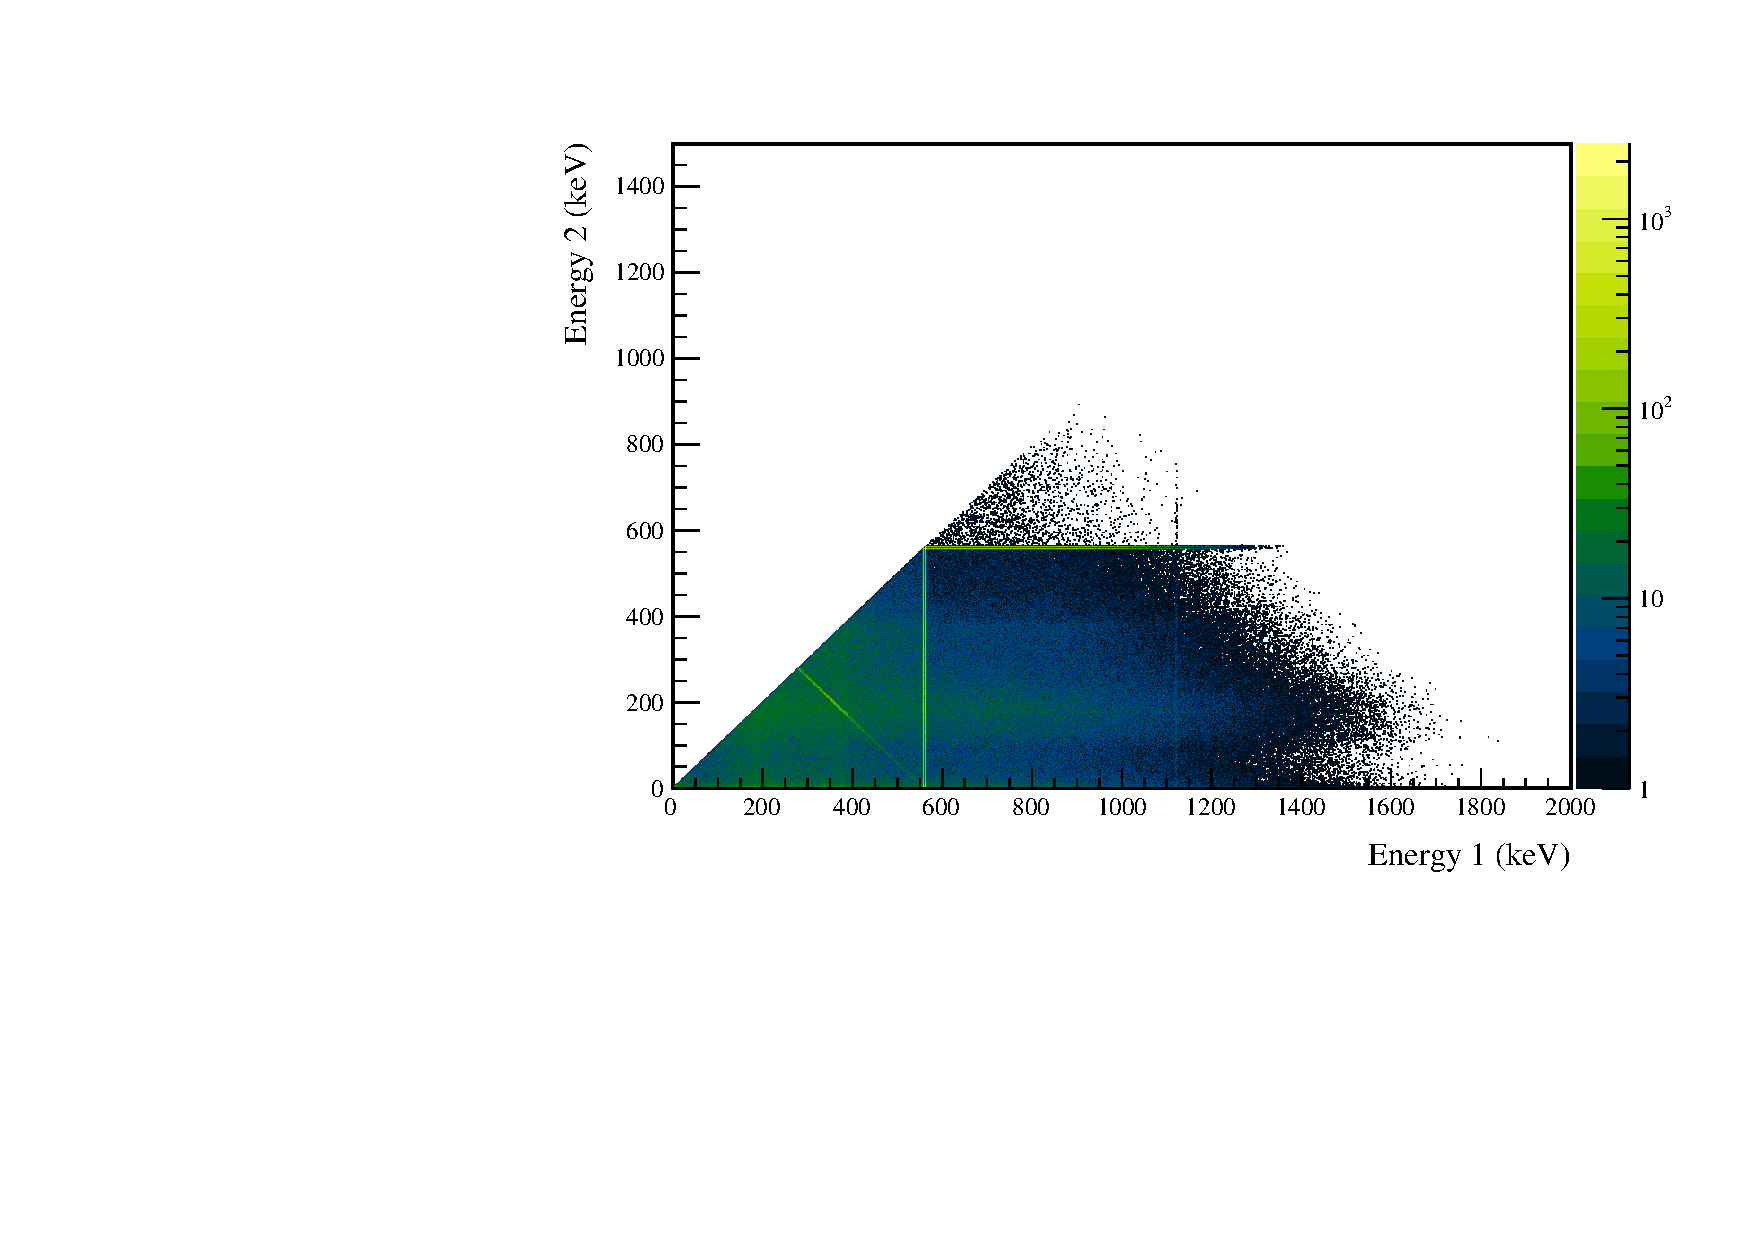
\includegraphics[width=.8\linewidth]{ESsim_2vBB_ES0_1}
  \caption[Simulation of \tnbb\ to \SP{0}{+}{1}]{
    Simulated multiplicity 2 energy spectrum of the \tnbb\ to \SP{0}{+}{1} decay mode}
\end{figure}

\allmodeplots{2vBB_ES0_1}{\tnbb\ to \SP{0}{+}{1}}{559~and 563~keV peaks}

\section{\tnbb\ to \SP{2}{+}{1}}
\begin{figure}[!htb]
  \centering
  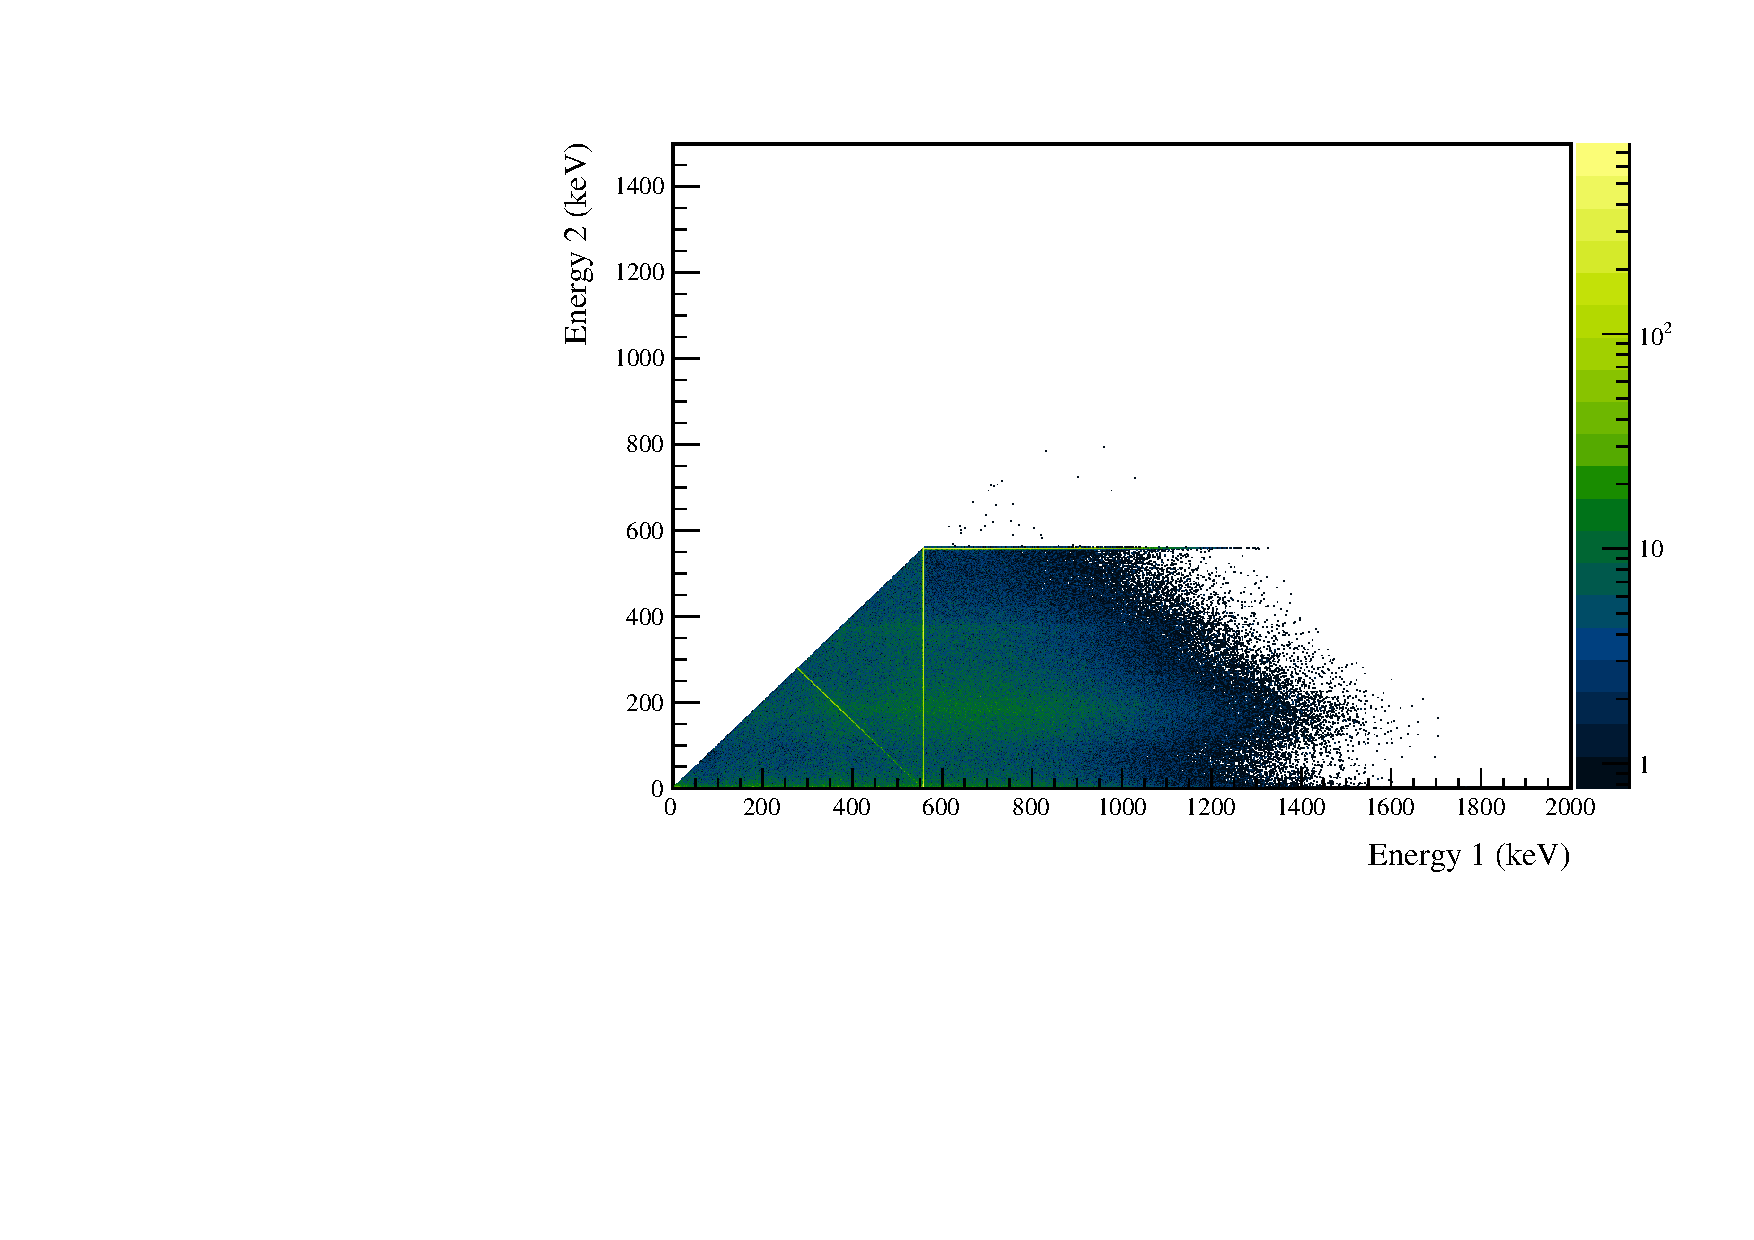
\includegraphics[width=.8\linewidth]{ESsim_2vBB_ES2_1}
  \caption[Simulation of \tnbb\ to \SP{2}{+}{1}]{
    Simulated multiplicity 2 energy spectrum of the \tnbb\ to \SP{2}{+}{1} decay mode}
\end{figure}

\allmodeplots{2vBB_ES2_1}{\tnbb\ to \SP{2}{+}{1}}{559~keV peak}

\section{\tnbb\ to \SP{2}{+}{2}}
\begin{figure}[!htb]
  \centering
  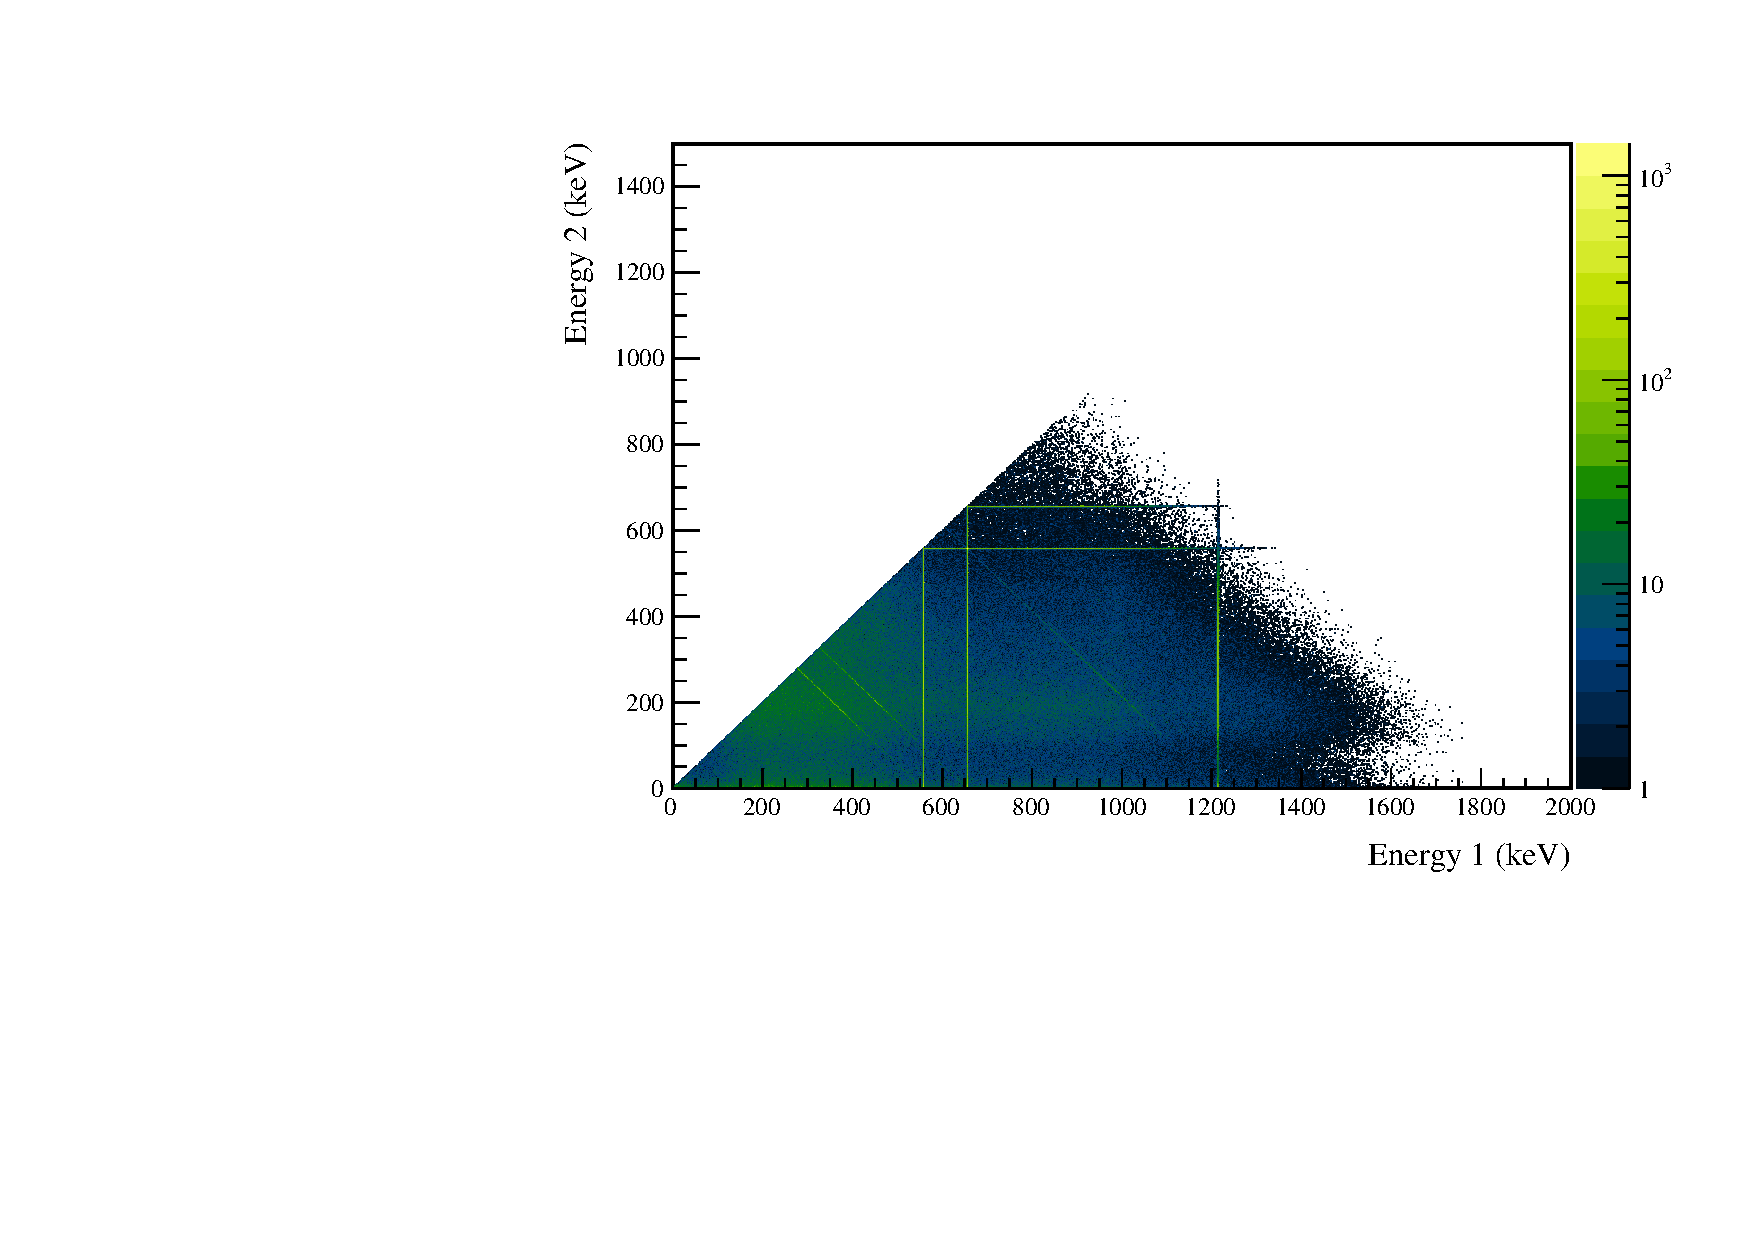
\includegraphics[width=.8\linewidth]{ESsim_2vBB_ES2_2}
  \caption[Simulation of \tnbb\ to \SP{2}{+}{2}]{
    Simulated multiplicity 2 energy spectrum of the \tnbb\ to \SP{2}{+}{2} decay mode}
\end{figure}

\subsection{559 keV peak}
\allmodeplots{2vBB_ES2_2_559}{\tnbb\ to \SP{2}{+}{2}}{559~keV peak}
\subsection{657 keV peak}
\allmodeplots{2vBB_ES2_2_657}{\tnbb\ to \SP{2}{+}{2}}{657~keV peak}
\subsection{1216 keV peak}
\allmodeplots{2vBB_ES2_2_1216}{\tnbb\ to \SP{2}{+}{2}}{1216~keV peak}



\section{\znbb\ to \SP{0}{+}{1}}
Note that both the 559~and 563~keV peaks will be shown together since they use the same sets of cuts.
\begin{figure}[!htb]
  \centering
  \includegraphics[width=.8\linewidth]{ESsim_0vBB_ES0_1}
  \caption[Simulation of \znbb\ to \SP{0}{+}{1}]{
    Simulated multiplicity 2 energy spectrum of the \znbb\ to \SP{0}{+}{1} decay mode}
\end{figure}

\allmodeplots{0vBB_ES0_1}{\znbb\ to \SP{0}{+}{1}}{559~and 563~keV peaks}

\section{\znbb\ to \SP{2}{+}{1}}
\begin{figure}[!htb]
  \centering
  \includegraphics[width=.8\linewidth]{ESsim_0vBB_ES2_1}
  \caption[Simulation of \znbb\ to \SP{2}{+}{1}]{
    Simulated multiplicity 2 energy spectrum of the \znbb\ to \SP{2}{+}{1} decay mode}
\end{figure}

\allmodeplots{0vBB_ES2_1}{\znbb\ to \SP{2}{+}{1}}{559~keV peak}

\section{\znbb\ to \SP{2}{+}{2}}
\begin{figure}[!htb]
  \centering
  \includegraphics[width=.8\linewidth]{ESsim_0vBB_ES2_2}
  \caption[Simulation of \znbb\ to \SP{2}{+}{2}]{
    Simulated multiplicity 2 energy spectrum of the \znbb\ to \SP{2}{+}{2} decay mode}
\end{figure}

\subsection{559 keV peak}
\allmodeplots{0vBB_ES2_2_559}{\znbb\ to \SP{2}{+}{2}}{559~keV peak}
\subsection{657 keV peak}
\allmodeplots{0vBB_ES2_2_657}{\znbb\ to \SP{2}{+}{2}}{657~keV peak}
\subsection{1216 keV peak}
\allmodeplots{0vBB_ES2_2_1216}{\znbb\ to \SP{2}{+}{2}}{1216~keV peak}




\section{Sensitivity and Discovery Potential}
\label{app:sens}

When performing rare event searches in the presence of backgrounds, it is often useful to select regions of interest and data cleaning cuts that optimize the experimental sensitivity.
Median n-$\sigma$ count sensitivity, $\hat{S}(\overline{B}, n_\sigma)$ is defined as the median upper limit of an n-$\sigma$ confidence interval on the number of observed signal counts, assuming the presence of no signal and backgrounds sampled from a distribution based on measured background level $\overline{B}$.
A similar quantity, n-$\sigma$ discovery sensitivity, is defined as the true strength of a signal that would produce a discovery with significance n-$\sigma$ 50\% of the time.
Unlike median sensitivity, discovery sensitivity accounts for the distribution in the number of counts that would be seen based on the true rate.
For this reason, discovery sensitivity is a slightly more useful quantity when projecting or optimizing an experiment's sensitivity, even though median (or mean) sensitivity is the quantity that is usually reported.
For the purpose of this appendix, we will focus on discovery sensitivity.

The sensitivity of the experiment to the total rate of the process being searched for is
\begin{equation}
  \hat{\Gamma}(\overline{B}, \epsilon, n_\sigma)\propto\frac{\hat{S}(\overline{B}, n_\sigma)}{\epsilon}
\end{equation}
where $\epsilon$ is the total detection efficiency of the signal being sought.
Optimizing event selection for a search requires balancing the tradeoff between reducing backgrounds, which will decrease $\hat{S}(\overline{B})$, and improving signal detection efficiency.

When optimizing a search, it is useful to use certain approximations when calculating sensitivity.
In the high background limit, a common approximation is to assume the backgrounds measured will have a gaussian distribution with standard deviation of $\sqrt{\overline{B}}$.
In this case, the discovery (and median) sensitivity will be
\begin{equation}
  \hat{S}(\overline{B}, n_\sigma)=n_\sigma * \sqrt{\overline{B}}
\end{equation}

This approximation fails, however, in the low background limit, where a better approximation is that the background will instead be sampled from a Poisson distribution with mean counts $\overline{B}$.
Because the Poisson distribution is a PDF over a discrete variable, the resultent sensitivity will have step-like properties and must be solved for using a toy Monte Carlo, properties that are not ideal for performing sensitivity optimizations.
For this reason, when computing the sensitivity we instead use the analytic continuation of the CDF of the poisson distribution, which is the lower incomplete gamma function
\begin{equation}
  \gamma(s, x)=\frac{1}{\Gamma(s)}\int_0^x t^{s-1} \mathrm{e}^{-t} \mathrm{d}t
\end{equation}
In this case, we can find the sensitivity, by first numerically solving for the number of counts required for an n-sigma discovery, $\hat{N}$, with expected backgrounds $\overline{B}$, where
\begin{equation}
  \gamma(\hat{N}+1, \overline{B}) = \mathrm{erfc}(\frac{n_\sigma}{\sqrt{2}})
\end{equation}
To get the median sensitivity, we then numerically solve
\begin{equation}
  \gamma(\hat{N}+1, \overline{B} + \hat{S}) = 0.5
\end{equation}
We define the function found by solving these equations to be the discovery potential\cite{2013CUORE},
\begin{equation}
  \hat{S}(\overline{B}, n_\sigma) = \mathrm{DP}(\overline{B}, n_\sigma)
\end{equation}
For the purposes of this dissertation, we always use the 3-sigma discovery potential
\begin{equation}
  \mathrm{DP}(\overline{B}) = \mathrm{DP}(\overline{B}, 3)
\end{equation}
Figure~\ref{fig:DPvSens} shows a comparison of the gaussian approximation for sensitivity to the discovery potential.
This function is implemented in \texttt{GATPeakShapeUtils.hh} as \linebreak\texttt{GATPeakShapeFunction::DiscoveryLimit}.

\begin{figure}[h]
  \centering
  \includegraphics[width=0.8\textwidth]{DPvSens}
  \caption{\label{fig:DPvSens}
    A comparison of the Gaussian approximation for sensitivity and the discovery potential as a function of expected background level. Note that in the high background limit, both formulations for sensitivity converge, as expected.
    }
\end{figure}
Next, we want to figure out how we will use these quantities to optimize our data selection.
To determine whether it is worth adding a cut or modifying a cut, consider the efficiency and expected background counts before and after applying the cut ($\epsilon_i$, $\overline{B}_i$ and $\epsilon_f$, $\overline{B}_f$, respectively).
A cut represents an improvement if
\begin{equation}
  \frac{\hat{S}(\overline{B}_f)}{\epsilon_f} <\frac{\hat{S}(\overline{B}_i)}{\epsilon_i}
\end{equation}
Rearranging this, we get
\begin{equation}
  \frac{\Delta \hat{S}(\overline{B})}{\hat{S}(\overline{B_i})} < \frac{\Delta\epsilon}{\epsilon_i}
\end{equation}
If we assume that a small number of events are cut, we can Taylor expand:
\begin{equation} \label{eq:cutcriterion}
  \frac{\partial\hat{S}}{\partial\overline{B}} \frac{\Delta\overline{B}}{\hat{S}(\overline{B})} < \frac{\Delta\epsilon}{\epsilon}
\end{equation}
\begin{equation}
  \frac{\partial\log(\hat{S})}{\partial\log(\overline{B})} > \frac{\mathrm{False~Positive~Rate}}{\mathrm{True~Positive~Rate}}
\end{equation}
Looking at figure~\ref{fig:DPvSens}, we see that in the high background limit, using the Gaussian sensitivity approximation we will draw the same conclusion about whether or not a cut is worth applying regardless of the absolute background level.
A cut is worth applying as long as the true positive rate of the cut is twice the true negative rate.
On the other hand, in the low background limit, this is not the case; instead, as we approach zero background, we will be less aggressive in cutting events.
For this reason, experiments approaching the background free limit will use wider regions of interest in peak searches.



\end{document}